\documentclass[11pt]{article}
\usepackage[margin=1in]{geometry}
\usepackage{amsmath,amssymb,mathtools,bm}
\usepackage{booktabs}
\usepackage{graphicx}
\usepackage{float}
\usepackage{microtype}
\usepackage{hyperref}
\usepackage{natbib}
\usepackage{xcolor}

\hypersetup{colorlinks=true,linkcolor=blue!55!black,citecolor=blue!55!black,urlcolor=blue!55!black,pdftitle={Resurgent Asymptotics of Rare-Event Tails in the Heston Model},pdfauthor={Rodrigo Varela}}
\newcommand{\E}{\mathbb E}
\newcommand{\Pp}{\mathbb P}
\newcommand{\R}{\mathbb R}
\newcommand{\C}{\mathbb C}
\newcommand{\dd}{\mathrm d}
\newcommand{\e}{\mathrm e}
\newcommand{\ii}{\mathrm i}
\newcommand{\calB}{\mathcal B}
\newcommand{\PhiH}{\Phi}

\title{Resurgent Asymptotics of Rare-Event Tails in the Heston Model:\\Borel Singularities, Stokes Data, and Caustic Continuation}
\author{Rodrigo Varela}
\date{September 2026}

\begin{document}
\maketitle

\begin{abstract}
We test whether rare-event saddles in a classical stochastic-volatility model leave the large-order and Borel signatures expected from resurgent asymptotics.  The object is a uniformly small-noise Heston left-tail probability.  The affine transform is exact in the scaled form $\E[\exp(pX_T/\varepsilon)]=\exp[\Lambda(p)/\varepsilon]$, so the probability is a one-dimensional Laplace-type integral whose saddle geometry can be studied independently of its perturbative expansion.

At a benchmark parameter point, the physical affine saddle, a separate Freidlin--Wentzell Hamiltonian shooting problem, and the large-order coefficients recover the same leading large-deviation scale.  The leading Borel obstruction is identified with the explicit CDF pole at $p=0$.  Continuing through the first negative Heston moment singularity yields an adjacent logarithmic-sheet saddle with singulant $\Delta S_1=2.792240162467\pm2.482246047281\,\ii$.  High-order coefficients locate the associated secondary Borel singularity independently: a 75-coefficient late-order fit is within $0.33\%$ of the continued action.  The local fluctuation series around the adjacent saddle reconstructs the lateral Borel jump, while residue summation of the conformal-Pad\'e pole condensation gives $S_{\rm lateral}=-0.998566+0.001484\,\ii$.  A separate Picard--Lefschetz calculation finds an oriented intersection jump $0\to-1$, fixing the same connection integer $S_{01}=-1$ geometrically.

We then continue the construction in parameter space.  On the tested nondegenerate domain, the logarithmic monodromy obeys $\operatorname{Im}\Delta S_1=2\pi\kappa\theta/\xi^2$ to numerical precision and the thimble intersection integer remains $-1$.  The continuation reveals a fold caustic where two real adjacent saddles coalesce and become a complex-conjugate pair, as well as anti-Stokes boundaries where exponential dominance changes.  A Chester--Friedman--Ursell reduction gives the expected square-root saddle splitting, three-halves action splitting, and an Airy uniform approximation through the fold.  Beyond the caustic, the lifted complex actions, local fluctuation sectors, and Borel singularities continue coherently.

The result is therefore not a claim that financial markets are quantum systems, nor a global theorem for all Heston parameters.  It is numerical and geometric evidence that this specific small-noise Heston tail observable admits a local resurgent description organised by saddle actions, Borel singularities, Stokes data, caustics, and anti-Stokes boundaries.
\end{abstract}

\section{Motivation and scope}
Path integrals, saddle points, response fields and generating functions are not exclusive to quantum theory. They also arise naturally in classical stochastic dynamics. Financial diffusions are therefore legitimate objects on which to test tools associated with semiclassical and resurgent analysis. Path-integral formulations of stochastic-volatility models have long been known \citep{baaquie2002,contreras2014}; merely rewriting Heston in path-integral language is not a new result.

The sharper question is whether the asymptotic perturbative sector of a financial observable contains quantitative information about rare, non-perturbative trajectories. In ordinary saddle-point problems, high-order perturbative coefficients can be governed by adjacent saddles and contour singularities. Resurgence organises this statement through the Borel plane, action differences, Stokes data and transseries sectors \citep{berry1991,aniceto2019}. Independently, small-noise diffusions admit Freidlin--Wentzell large-deviation principles, and the Heston model is known to support sample-path large deviations and asymptotically optimal importance-sampling controls \citep{robertson2010,geha2024}.

The central hypothesis of this project is therefore
\begin{quote}
\emph{rare-event saddles and analytic obstructions of stochastic financial models control the large-order behaviour and Borel singularities of suitable small-noise expansions.}
\end{quote}
We treat this as a falsifiable hypothesis. A divergent series is not by itself evidence for an instanton. A Pad\'e pole is not automatically a physical saddle. A factorial series is not automatically a renormalon. Whenever possible, non-perturbative quantities are calculated independently of the perturbative coefficients they are compared with.

\section{Resurgent diagnostic for a saddle expansion}
Consider an observable with formal expansion
\begin{equation}
F(g)\sim\sum_{n\ge0}a_n g^n.
\end{equation}
If the coefficients have large-order form
\begin{equation}
 a_n\sim C\,\frac{\Gamma(n+\beta)}{A^{n+\beta}}
 \left(1+\frac{a^{(1)}}{n}+\frac{a^{(2)}}{n^2}+\cdots\right),
 \label{eq:largeorder}
\end{equation}
then the Borel transform
\begin{equation}
 \calB F(\zeta)=\sum_{n\ge0}\frac{a_n}{n!}\zeta^n
 \label{eq:borel}
\end{equation}
has a singularity at a scale set by $A$. In a resurgent saddle problem, $A$ is typically an action difference, or more generally the singulant between the expansion point and an adjacent saddle or contour obstruction \citep{berry1991,aniceto2019}.

A basic finite-order estimator is
\begin{equation}
 A_n=n\frac{a_{n-1}}{a_n},
 \label{eq:ratio}
\end{equation}
with the sign retained. The Borel transform is analytically continued with near-diagonal Pad\'e approximants. When the positive Borel ray is unobstructed, the resummed series is evaluated by
\begin{equation}
 \mathcal S F(g)=\int_0^\infty \e^{-t}\,\calB F(gt)\,\dd t.
 \label{eq:borellaplace}
\end{equation}
In the numerical implementation the last integral is computed by Gauss--Laguerre quadrature. For a Stokes direction $\vartheta$, lateral sums are defined by deforming the Borel--Laplace contour above and below the ray $\arg\zeta=\vartheta$. Their difference is the Stokes discontinuity; in a finite Pad'e approximation a logarithmic cut is represented by a condensation of simple poles, so the lateral jump may be evaluated by a residue sum.

The working criterion used throughout the project is deliberately strict: a Borel singularity receives a non-perturbative interpretation only if its location is stable under approximation order and agrees with an independently calculated action difference or analytic obstruction.

\section{Benchmark I: Gaussian rare-event tail}
Before studying Heston, it is useful to test the entire pipeline on a tail probability where both the non-perturbative exponential and the Borel transform are known exactly. Let
\begin{equation}
 X_T=m+\sigma\sqrt{\varepsilon T}\,Z,
 \qquad Z\sim\mathcal N(0,1),
\end{equation}
and choose a fixed left-tail threshold $x_\star<m$. Define
\begin{equation}
 A=\frac{(m-x_\star)^2}{2\sigma^2T}.
\end{equation}
Then
\begin{equation}
 \Pp(X_T\le x_\star)=\frac12\operatorname{erfc}\!\left(\sqrt{A/\varepsilon}\right).
\end{equation}
Its small-noise expansion is
\begin{equation}
 \Pp(X_T\le x_\star)
 \sim \e^{-A/\varepsilon}\frac{\sqrt\varepsilon}{2\sqrt{\pi A}}
 \sum_{n\ge0}c_n\varepsilon^n,
\end{equation}
with
\begin{equation}
 c_n=(-1)^n\frac{\Gamma(n+1/2)}{\sqrt\pi\,A^n}.
\end{equation}
The fluctuation series is factorially divergent and its Borel transform is exactly
\begin{equation}
 \calB(\zeta)=\left(1+\frac{\zeta}{A}\right)^{-1/2},
\end{equation}
so the leading branch point is $\zeta=-A$.

For the repository benchmark, $A=1.125$. The order-ratio diagnostic approaches $-A$ and Borel--Pad\'e reconstructs the exact probability to approximately $10^{-9}$ maximum relative error over the tested grid. This verifies the sign convention, coefficient normalisation, Pad\'e construction and Borel--Laplace implementation.

\begin{figure}[H]
\centering
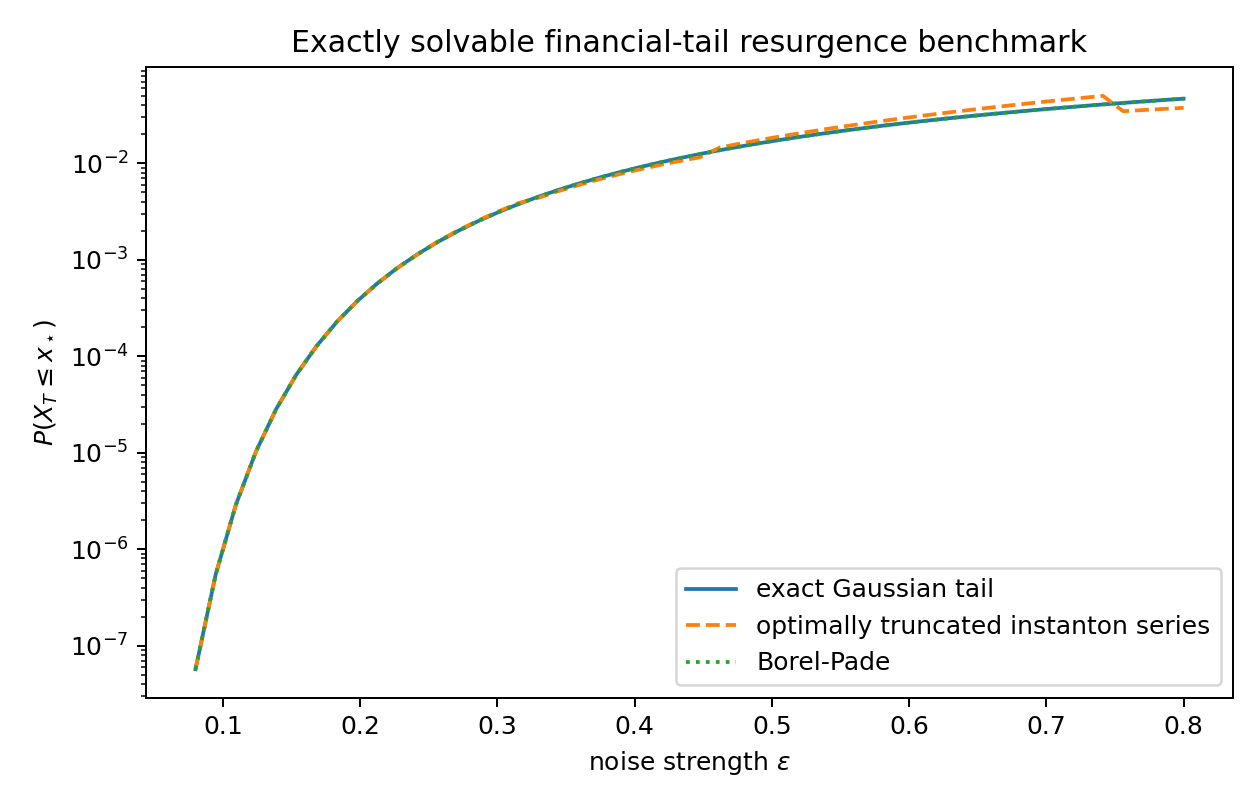
\includegraphics[width=0.78\textwidth]{../figures/gaussian_tail_resummation.png}
\caption{Gaussian validation. Exact left-tail probability compared with optimally truncated asymptotics and Borel--Pad\'e resummation.}
\label{fig:gaussian}
\end{figure}

\section{Benchmark II: nonlinear quartic factor}
A second benchmark is needed to verify that perturbative coefficients can recover a genuinely nontrivial complex saddle. We use
\begin{equation}
 Z(g)=\frac{1}{\sqrt\pi}\int_{-\infty}^{\infty}\e^{-x^2-gx^4}\,\dd x,
 \qquad g>0.
 \label{eq:quartic}
\end{equation}
This is used as a zero-dimensional nonlinear factor model, not as an empirical distribution for returns. Its formal perturbative coefficients are
\begin{equation}
 a_n=(-1)^n\frac{\Gamma(2n+1/2)}{\sqrt\pi\,n!}.
\end{equation}
The exponent has stationary points
\begin{equation}
 x_0=0,
 \qquad x_\pm=\pm\frac{\ii}{\sqrt{2g}},
\end{equation}
and the corresponding action difference implies a Borel scale
\begin{equation}
 A=-\frac14.
\end{equation}
The exact integral is
\begin{equation}
 Z(g)=\frac{\e^{1/(8g)}}{2\sqrt{\pi g}}K_{1/4}\!\left(\frac{1}{8g}\right).
\end{equation}
The current implementation finds a large-order estimate near $-0.2573$ and a nearest Pad\'e singularity near $-0.2544$, converging toward $-1/4$. Borel--Pad\'e agrees with the exact integral at roughly $10^{-8}$ maximum relative error on the test interval. This benchmark establishes that the numerical pipeline can recover the scale of a nontrivial complex saddle from perturbative data.

\begin{figure}[H]
\centering
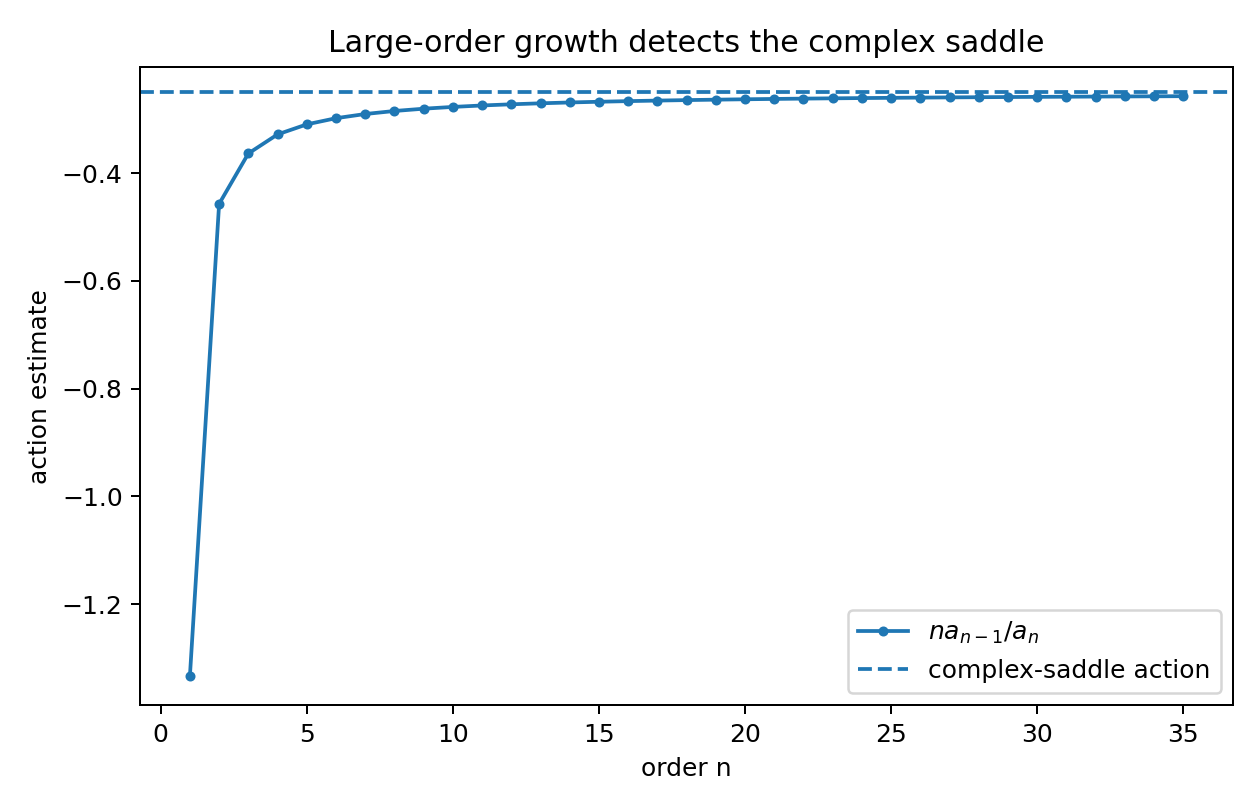
\includegraphics[width=0.78\textwidth]{../figures/quartic_factor_large_order.png}
\caption{Large-order diagnostic for the nonlinear quartic benchmark. The exact complex-saddle scale is $-1/4$.}
\label{fig:quartic}
\end{figure}

\section{Uniform small-noise Heston dynamics}
Let $X_t=\log(S_t/S_0)$ and introduce a uniform noise parameter $\varepsilon>0$,
\begin{align}
 \dd X_t&=\left(\mu-\frac12V_t\right)\dd t+\sqrt{\varepsilon V_t}\,\dd W_t^{(1)},\label{eq:hestonx}\\
 \dd V_t&=\kappa(\theta-V_t)\dd t+\sqrt\varepsilon\,\xi\sqrt{V_t}\,\dd W_t^{(2)},\label{eq:hestonv}
\end{align}
with
\begin{equation}
 \dd W_t^{(1)}\dd W_t^{(2)}=\rho\,\dd t.
\end{equation}
The small-noise scaling is natural for large-deviation analysis and is closely related to Heston importance-sampling asymptotics \citep{robertson2010,geha2024}.

\subsection{Freidlin--Wentzell action}
Writing $\bm y=(x,v)$, the drift and covariance matrix are
\begin{equation}
 \bm b(x,v)=
 \begin{pmatrix}
 \mu-v/2\\
 \kappa(\theta-v)
 \end{pmatrix},
 \qquad
 a(v)=v
 \begin{pmatrix}
 1&\rho\xi\\
 \rho\xi&\xi^2
 \end{pmatrix}.
\end{equation}
For an absolutely continuous path $\bm y(t)$ with positive variance, the Freidlin--Wentzell action is
\begin{equation}
 S[\bm y]=\frac12\int_0^T
 (\dot{\bm y}-\bm b)^T a^{-1}(v)(\dot{\bm y}-\bm b)\,\dd t.
 \label{eq:FWaction}
\end{equation}
A rare endpoint is exponentially weighted as
\begin{equation}
 \Pp(X_T\approx x_\star)\asymp\exp[-I(x_\star)/\varepsilon],
\end{equation}
where the rate $I$ is the minimum of \eqref{eq:FWaction} under the endpoint constraint.

The corresponding Hamiltonian is
\begin{align}
 H(x,v,p_x,p_v)=&\;p_x\left(\mu-\frac v2\right)
 +p_v\kappa(\theta-v)\nonumber\\
 &+\frac v2\left(p_x^2+2\rho\xi p_xp_v+\xi^2p_v^2\right).
 \label{eq:Hamiltonian}
\end{align}
Hamilton's equations are
\begin{align}
 \dot x&=\mu-\frac v2+v(p_x+\rho\xi p_v),\\
 \dot v&=\kappa(\theta-v)+v(\rho\xi p_x+\xi^2p_v),\\
 \dot p_x&=0,\\
 \dot p_v&=\frac12p_x+\kappa p_v
 -\frac12\left(p_x^2+2\rho\xi p_xp_v+\xi^2p_v^2\right).
 \label{eq:Hameqs}
\end{align}
For the event $X_T=x_\star$ with unconstrained terminal variance, the transversality conditions are
\begin{equation}
 x(0)=0,\qquad v(0)=v_0,\qquad x(T)=x_\star,\qquad p_v(T)=0.
\end{equation}
Since $p_x$ is constant, the numerical shooting problem is effectively one-dimensional: integrate $p_v$ backwards from $T$, then $(x,v)$ forwards, and choose $p_x$ so that $x(T)=x_\star$. The action can equivalently be reconstructed from
\begin{equation}
 S=\int_0^T\left(\bm p\cdot\dot{\bm y}-H\right)\dd t.
\end{equation}

\section{Exact scaled affine transform}
The decisive simplification of the chosen scaling is that the scaled moment-generating function has an exact WKB form rather than merely an asymptotic one.

Let
\begin{equation}
 M(\tau,x,v;p)=\E_{x,v}\left[\exp\left(\frac{pX_\tau}{\varepsilon}\right)\right].
\end{equation}
The backward generator of \eqref{eq:hestonx}--\eqref{eq:hestonv} contains the diffusion terms multiplied by $\varepsilon$. Use the affine ansatz
\begin{equation}
 M(\tau,x,v;p)=
 \exp\left[\frac{px+c(\tau,p)+d(\tau,p)v}{\varepsilon}\right].
 \label{eq:affineansatz}
\end{equation}
Substitution into the backward equation and collection of the coefficients of $v$ and the constant term give
\begin{align}
 \dot d&=\frac12(p^2-p)+(\rho\xi p-\kappa)d+\frac12\xi^2d^2,
 \qquad d(0,p)=0,\label{eq:riccati}\\
 \dot c&=\mu p+\kappa\theta d,
 \qquad c(0,p)=0.\label{eq:cRiccati}
\end{align}
There is no remaining $\varepsilon$ dependence in these equations. Consequently, for $X_0=0$,
\begin{equation}
 \boxed{
 \E\left[\exp\left(\frac{pX_T}{\varepsilon}\right)\right]
 =\exp\left[\frac{\Lambda(p)}{\varepsilon}\right]},
 \qquad
 \Lambda(p)=c(T,p)+v_0d(T,p).
 \label{eq:scaledtransform}
\end{equation}
This exact scaling is what makes high-order asymptotics especially clean in this model.

The Riccati solution can be written in closed form. Define
\begin{equation}
 B(p)=\kappa-\rho\xi p,
 \qquad
 \gamma(p)=\sqrt{B(p)^2-\xi^2(p^2-p)},
 \qquad
 g(p)=\frac{B(p)-\gamma(p)}{B(p)+\gamma(p)}.
\end{equation}
Then
\begin{equation}
 d_T(p)=\frac{B-\gamma}{\xi^2}
 \frac{1-\e^{-\gamma T}}{1-g\e^{-\gamma T}},
 \label{eq:dclosed}
\end{equation}
and
\begin{align}
 \Lambda(p)=&\;\mu pT+v_0d_T(p)\nonumber\\
 &+\frac{\kappa\theta}{\xi^2}
 \left[(B-\gamma)T-2\log\left(\frac{1-g\e^{-\gamma T}}{1-g}\right)\right].
 \label{eq:Lambdaclosed}
\end{align}
This is the small-noise-scaled version of the affine transform underlying the original Heston solution \citep{heston1993}. The locations at which the Riccati denominator vanishes are moment-explosion singularities of the affine transform; such critical moments are a standard feature of affine stochastic-volatility models \citep{kellerressel2011}.

\section{Tail probability as an exact steepest-descent integral}
For a fixed threshold $x_\star$ below the deterministic endpoint, inverse Laplace transformation gives
\begin{equation}
 F_\varepsilon(x_\star)
 =\Pp(X_T\le x_\star)
 =-\frac{1}{2\pi\ii}\int_{c-\ii\infty}^{c+\ii\infty}
 \frac{\dd p}{p}
 \exp\left[\frac{\Lambda(p)-px_\star}{\varepsilon}\right],
 \qquad c<0.
 \label{eq:bromwich}
\end{equation}
Introduce
\begin{equation}
 \PhiH(p)=\Lambda(p)-px_\star.
\end{equation}
The physical real saddle $p_\star<0$ satisfies
\begin{equation}
 \Lambda'(p_\star)=x_\star,
 \label{eq:saddleeq}
\end{equation}
and
\begin{equation}
 I(x_\star)=p_\star x_\star-\Lambda(p_\star)=-\PhiH(p_\star)>0.
 \label{eq:rate}
\end{equation}
Thus the contraction-principle large-deviation rate is simultaneously the saddle exponent of the exact affine inversion.

\subsection{Formal fluctuation expansion}
Set
\begin{equation}
 p=p_\star+\ii\sqrt{\frac{\varepsilon}{\Lambda''(p_\star)}}\,z,
 \qquad s=\sqrt\varepsilon.
\end{equation}
After extracting the Gaussian factor, \eqref{eq:bromwich} takes the form
\begin{equation}
 F_\varepsilon(x_\star)
 \sim \e^{-I/\varepsilon}
 \left(-\frac{1}{p_\star}\right)
 \sqrt{\frac{\varepsilon}{2\pi\Lambda''(p_\star)}}
 \sum_{n\ge0}c_n\varepsilon^n.
 \label{eq:hestonsaddleexp}
\end{equation}
The coefficients can be generated algebraically. Write
\begin{equation}
 Q(z,s)=\sum_{m\ge1}q_m z^{m+2}s^m,
\end{equation}
with
\begin{equation}
 q_m=
 \frac{\Lambda^{(m+2)}(p_\star)\,\ii^{m+2}}
 {(m+2)!\,[\Lambda''(p_\star)]^{(m+2)/2}}.
\end{equation}
The pole amplitude expands as
\begin{equation}
 \frac{p_\star}{p_\star+\ii s z/\sqrt{\Lambda''(p_\star)}}
 =\sum_{j\ge0}
 \left(-\frac{\ii z}{p_\star\sqrt{\Lambda''(p_\star)}}\right)^j s^j.
\end{equation}
Multiplying this series by $\exp Q$ and taking Gaussian moments
\begin{equation}
 \langle z^{2m}\rangle=(2m-1)!!,
 \qquad
 \langle z^{2m+1}\rangle=0,
\end{equation}
produces the $c_n$. The repository performs the algebra at arbitrary precision because the coefficients grow factorially and because secondary-singularity extraction is sensitive to cancellation.

For high perturbative order, repeatedly differentiating the closed affine expression becomes the computational bottleneck. We therefore extract the local Taylor coefficients of $\Lambda$ from Cauchy's formula,
\begin{equation}
 \frac{\Lambda^{(k)}(p_\star)}{k!}
 =\frac{1}{2\pi\ii}
 \oint_{|q-p_\star|=r}
 \frac{\Lambda(q)}{(q-p_\star)^{k+1}}\,\dd q,
 \label{eq:cauchytaylor}
\end{equation}
using a high-precision trapezoidal discretisation on a circle that remains inside the nearest affine branch point. For the benchmark, $r=0.25$ is safely below the distance to the closest discriminant singularity. This replacement reduces the 75-coefficient calculation to seconds while reproducing the earlier derivative-based coefficients through order 45 to the stored precision.

\section{Benchmark Heston parameters and independent instanton action}
We use
\begin{equation}
 \kappa=2,
 \quad\theta=v_0=0.04,
 \quad\xi=0.45,
 \quad\rho=-0.7,
 \quad\mu=0,
 \quad T=1,
 \quad x_\star=-0.25.
 \label{eq:params}
\end{equation}
Solving \eqref{eq:saddleeq} with the affine transform gives
\begin{equation}
 p_\star=-2.849561078040,
 \qquad
 I(x_\star)=0.396018751741,
 \qquad
 \Lambda''(p_\star)=0.154480122015.
 \label{eq:affineres}
\end{equation}
The Hamiltonian shooting calculation based only on \eqref{eq:Hamiltonian}--\eqref{eq:Hameqs} gives
\begin{equation}
 p_x=-2.849561078040,
 \qquad
 S_{\rm FW}=0.396018650224.
 \label{eq:hamres}
\end{equation}
The agreement of $p_x$ with the affine saddle and of $S_{\rm FW}$ with the contraction rate provides an independent non-perturbative validation.

\begin{figure}[H]
\centering
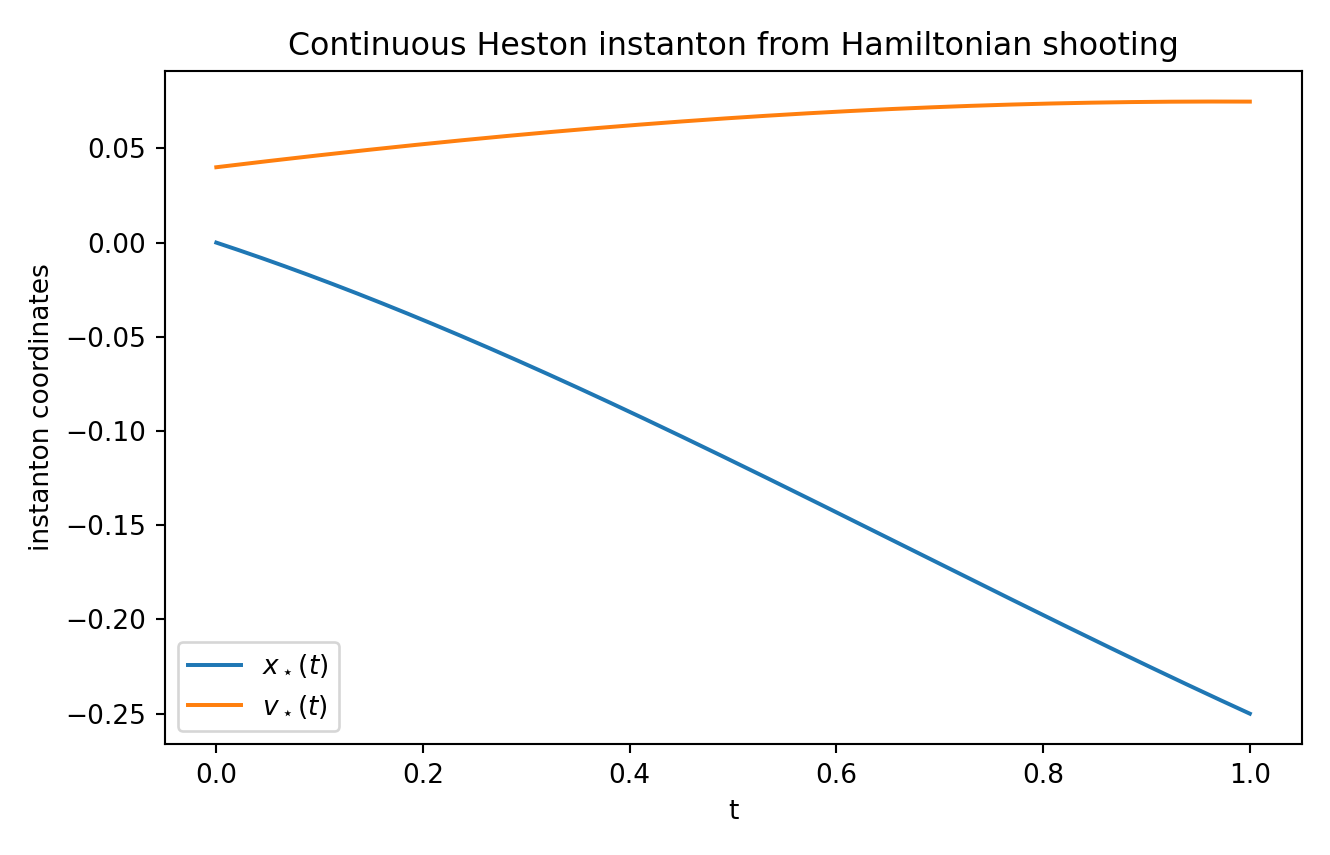
\includegraphics[width=0.78\textwidth]{../figures/heston_hamiltonian_instanton.png}
\caption{Continuous minimum-action Heston path obtained from Hamiltonian shooting.}
\label{fig:instanton}
\end{figure}

\section{Leading Heston large-order result}
The first coefficients of \eqref{eq:hestonsaddleexp} are
\begin{align}
 c_0&=1,\\
 c_1&=-1.599509864\ldots,\\
 c_2&=6.018681066\ldots,\\
 c_3&=-37.99045699\ldots,\\
 c_4&=335.7767025\ldots,
\end{align}
and the magnitude grows factorially. With 31 coefficients, the ratio sequence \eqref{eq:ratio}, fitted as a cubic polynomial in $1/n$ over the high-order window used in the repository, gives
\begin{equation}
 \zeta_{\rm LO}=-0.396018496470.
 \label{eq:leadingLO}
\end{equation}
The independently predicted leading Borel location is
\begin{equation}
 -I=-0.396018751741.
\end{equation}
The absolute difference is $2.55\times10^{-7}$.

\begin{figure}[H]
\centering
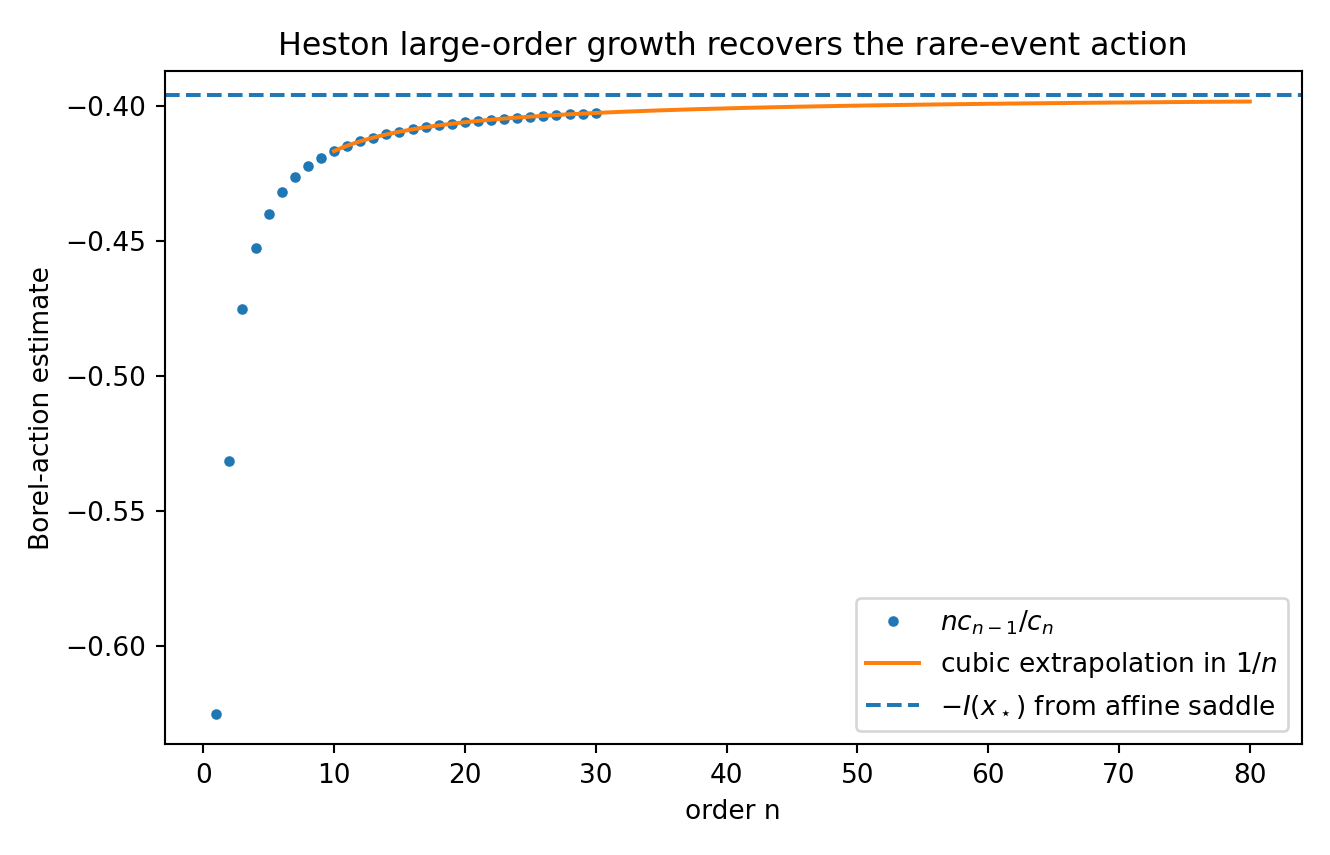
\includegraphics[width=0.8\textwidth]{../figures/heston_large_order_action.png}
\caption{The large-order ratio diagnostic recovers the independently calculated rare-event action scale.}
\label{fig:hestonlo}
\end{figure}

Pad\'e continuation of the Borel transform produces a sequence of poles approximating a cut on the negative real axis. D-log Pad\'e analysis gives a leading residue close to $-1/2$, consistent with the square-root type already seen in the Gaussian tail. The location of the cut endpoint agrees with $-I$.

\begin{figure}[H]
\centering
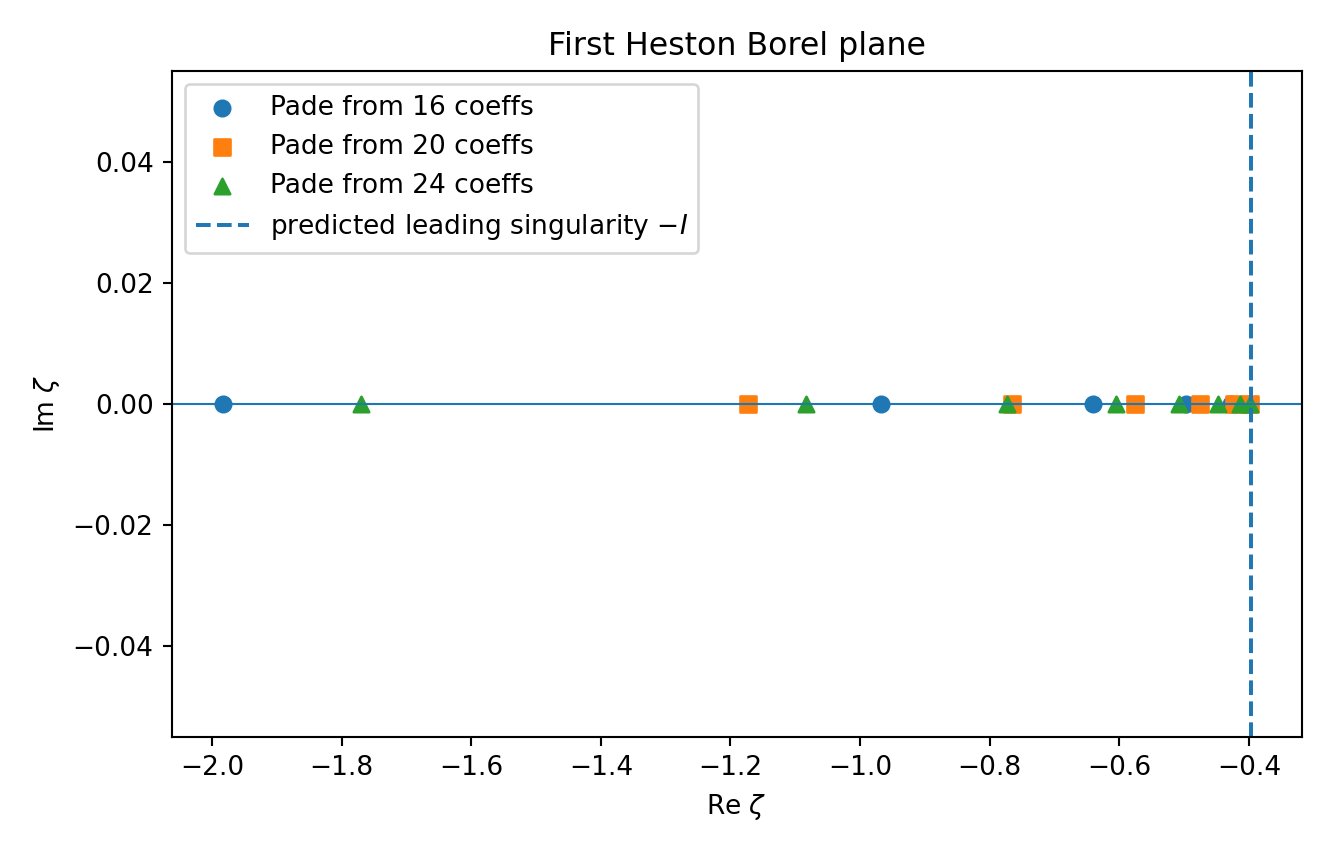
\includegraphics[width=0.8\textwidth]{../figures/heston_borel_plane.png}
\caption{Pad\'e representation of the first Heston Borel plane. The negative-axis pole condensation approaches $\zeta=-I$.}
\label{fig:hestonborel}
\end{figure}

\subsection{Why the leading singularity is not a second instanton}
The CDF integrand in \eqref{eq:bromwich} contains the explicit pole $1/p$. Since $\Lambda(0)=0$,
\begin{equation}
 \PhiH(p_\star)-\PhiH(0)=-I(x_\star).
 \label{eq:p0singulant}
\end{equation}
The observed leading Borel singularity is therefore naturally associated with the nearby contour obstruction at $p=0$. This is precisely the kind of mechanism by which adjacent saddles or singularities control late terms of a steepest-descent expansion \citep{berry1991}. The result is a genuine large-order/non-perturbative match, but calling the $-I$ singularity a second Heston instanton would be misleading.

\section{Borel resummation versus direct truncation}
The same affine transform supplies an essentially exact numerical reference: deform the Bromwich contour through $p_\star$, rescale its imaginary coordinate by $\sqrt\varepsilon$, and integrate the resulting rapidly decaying integrand. On the grid
\begin{equation}
 0.04\le\varepsilon\le0.8,
\end{equation}
a 24-coefficient Borel--Pad\'e resummation has maximum relative error
\begin{equation}
 \boxed{1.85\times10^{-4}},
\end{equation}
while the optimally truncated bare asymptotic series becomes order-one inaccurate at the large-$\varepsilon$ end of the interval. Thus the Borel construction is not merely identifying singularities: it materially extends the useful range of the small-noise asymptotics.

\begin{figure}[H]
\centering
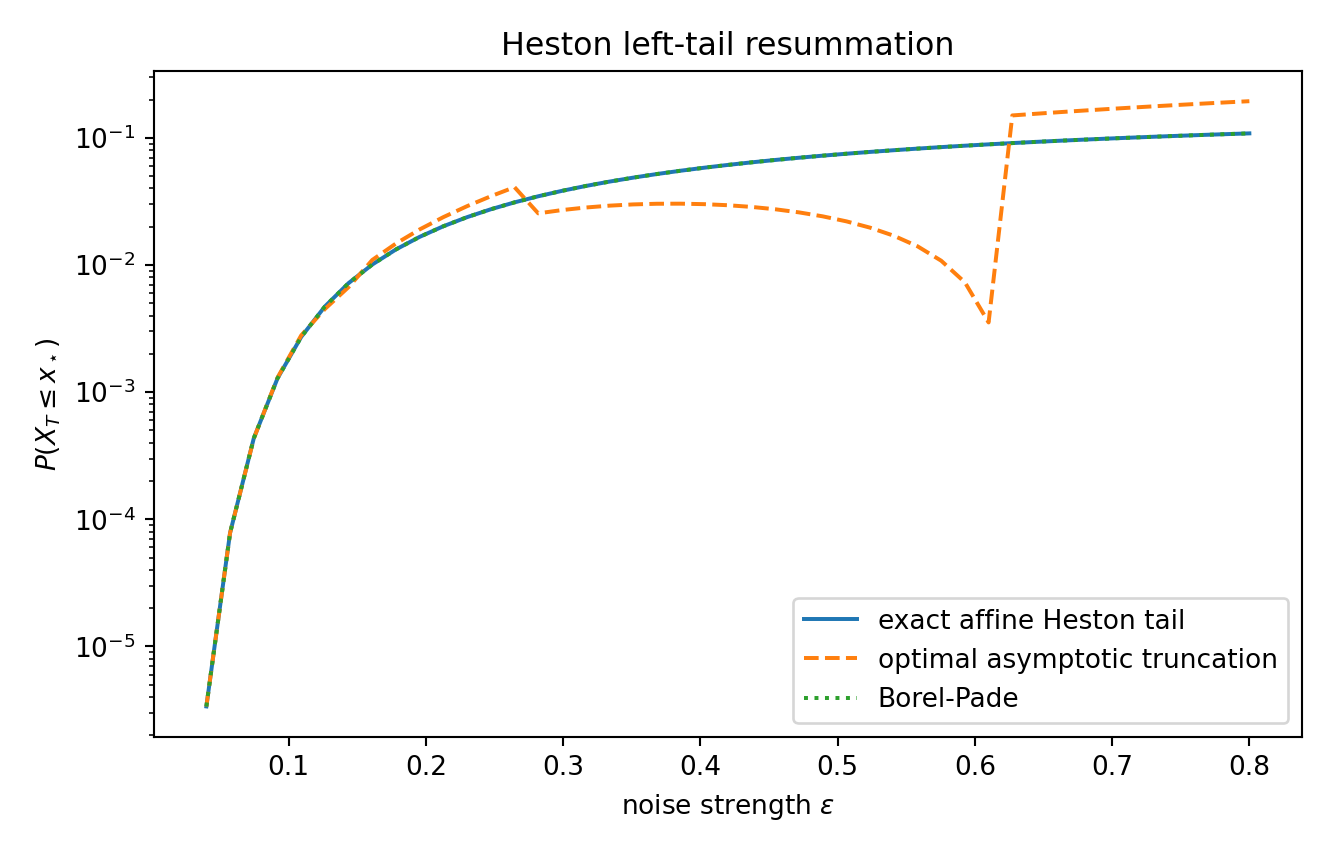
\includegraphics[width=0.8\textwidth]{../figures/heston_tail_resummation.png}
\caption{Exact affine tail, optimal asymptotic truncation and Borel--Pad\'e resummation.}
\label{fig:resum}
\end{figure}

\section{Analytic continuation beyond the first moment pole}
We now ask whether a secondary Borel singularity can be associated with a nontrivial stationary point on an adjacent analytic sheet.

\subsection{First negative moment pole}
The Riccati denominator in \eqref{eq:dclosed} vanishes when
\begin{equation}
 1-g(p)\e^{-\gamma(p)T}=0.
 \label{eq:momentpoleeq}
\end{equation}
For the benchmark parameters, the first negative real solution is
\begin{equation}
 \boxed{p_{\rm pole}=-6.453093949198}.
 \label{eq:firstpole}
\end{equation}
This is the first moment-explosion obstruction encountered when continuing from the physical negative-moment domain. Moment explosions and the resulting finite strip of analyticity are characteristic of affine stochastic-volatility transforms \citep{kellerressel2011}.

\subsection{Adjacent-sheet stationary point}
The derivative $\Lambda'(p)$ is insensitive to adding an integer branch constant to the logarithm in \eqref{eq:Lambdaclosed}. We may therefore continue the stationary equation
\begin{equation}
 \Lambda'(p)=x_\star
\end{equation}
through the first moment singularity and solve it on the next logarithmic sheet. The nearest stationary point found in this continuation is
\begin{equation}
 \boxed{p_1=-7.998322139804}.
 \label{eq:p1}
\end{equation}
It lies beyond the moment pole, as illustrated in Figure~\ref{fig:sheetstructure}.

\begin{figure}[H]
\centering
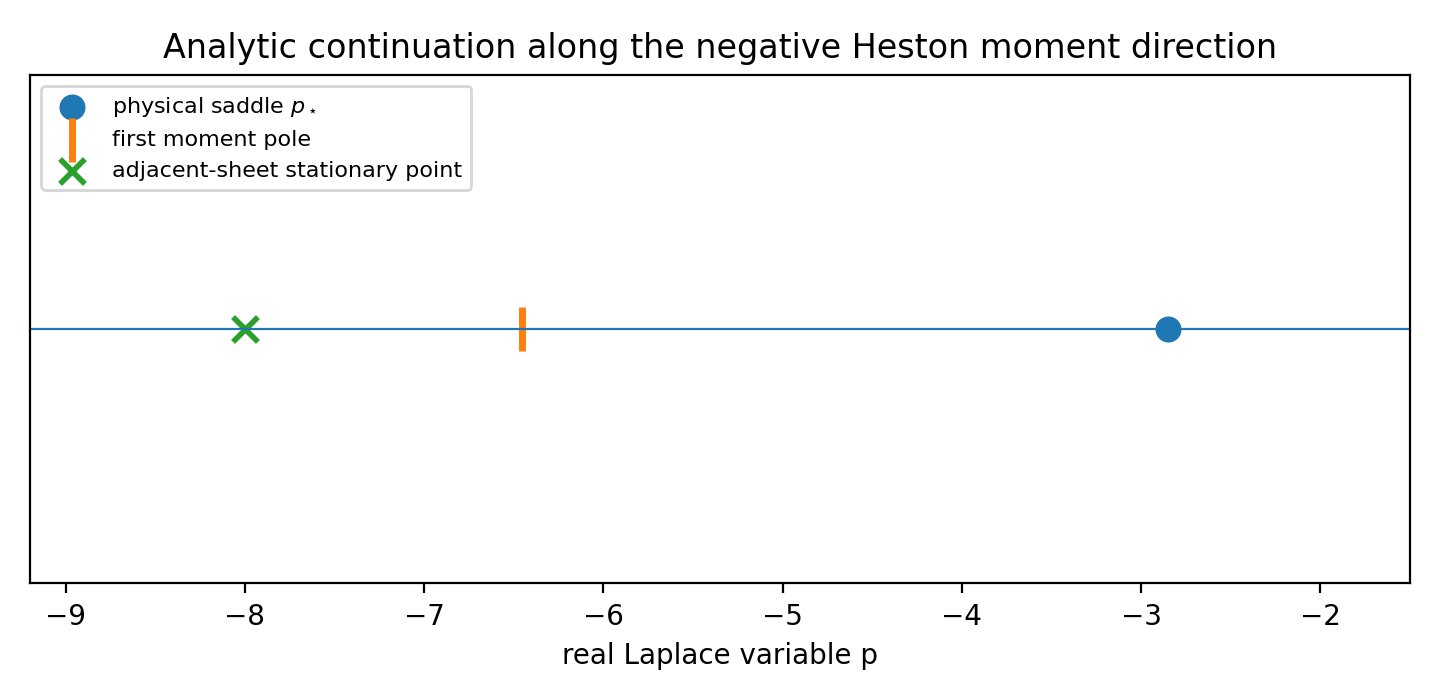
\includegraphics[width=0.82\textwidth]{../figures/heston_adjacent_sheet_structure.png}
\caption{Real-$p$ analytic structure relevant to the first adjacent sheet: physical saddle, first negative moment pole, and the stationary point reached after continuation.}
\label{fig:sheetstructure}
\end{figure}

Define the singulant using the analytically continued exponent,
\begin{equation}
 \Delta S_1=\PhiH(p_\star)-\PhiH_1(p_1).
 \label{eq:singulantdef}
\end{equation}
The numerical value is
\begin{equation}
 \boxed{
 \Delta S_1
 =2.792240162467+2.482246047281\,\ii},
 \label{eq:secondaryaction}
\end{equation}
with the opposite bypass of the logarithmic obstruction giving the conjugate value. The imaginary component is not arbitrary. At the zero of the logarithm in \eqref{eq:Lambdaclosed}, continuation on opposite sides changes the logarithmic phase by $\pm\pi$. Because the logarithm appears with coefficient $-2\kappa\theta/\xi^2$, the adjacent-sheet imaginary action is
\begin{equation}
 \left|\operatorname{Im}\Delta S_1\right|
 =2\pi\frac{\kappa\theta}{\xi^2}
 =2.482246047281.
 \label{eq:monodromy}
\end{equation}
This exact numerical equality is a useful check that the complex action is genuinely tied to the logarithmic sheet structure of the affine transform.

\section{Removing the leading Borel cut by conformal mapping}
The secondary pair in \eqref{eq:secondaryaction} is far outside the radius of convergence imposed by the leading singularity $\zeta=-I$. Direct Pad\'e approximants are consequently dominated by the negative-axis cut. We therefore use the standard one-cut conformal map
\begin{equation}
 w(\zeta)=
 \frac{\sqrt{1+\zeta/I}-1}{\sqrt{1+\zeta/I}+1},
 \qquad
 \zeta(w)=\frac{4Iw}{(1-w)^2}.
 \label{eq:conformal}
\end{equation}
It maps the Borel plane cut along $(-\infty,-I]$ to the unit disk and sends the branch point $-I$ to $w=-1$. The adjacent-sheet action \eqref{eq:secondaryaction} maps to
\begin{equation}
 w(\Delta S_1)
 =0.533659118251+0.120308808652\,\ii,
 \qquad
 |w|=0.547052341126.
 \label{eq:targetw}
\end{equation}
so a genuine secondary singularity at $\Delta S_1$ would sit well inside the conformal disk and should eventually dominate high-order coefficients of the transformed series.

A crucial numerical point is that the composition
\begin{equation}
 \calB F(\zeta(w))
\end{equation}
must be carried out at arbitrary precision. At orders $n\gtrsim30$, a direct double-precision composition suffers severe cancellation and produces spurious pole patterns. The repository therefore generates 60 Heston fluctuation coefficients and performs the Borel transform and conformal composition with multiprecision arithmetic before the final Pad\'e solve.

\section{Secondary Borel-plane result}
With 75 coefficients, the finite Pad\'e representation of the secondary logarithmic cut forms a short pole condensation. The pole nearest the independently predicted branch point is
\begin{equation}
 \boxed{
 \zeta_{\rm BP}^{(2)}
 =2.831243366402+2.504669377762\,\ii}.
 \label{eq:secondarypade}
\end{equation}
Its relative distance from the independently calculated adjacent-sheet action is
\begin{equation}
 \frac{|\zeta_{\rm BP}^{(2)}-\Delta S_1|}{|\Delta S_1|}
 =1.20\%.
 \label{eq:secondaryerror}
\end{equation}
The same selection at 55, 60, 65 and 70 coefficients shows a gradual reduction of the gap from roughly $2\%$ toward the 75-coefficient value.

Pad\'e pole locations are not the only way to infer the singularity. If the first residual singularity is logarithmic, the high-order conformal-Borel coefficients obey at leading order
\begin{equation}
 b_n\sim -2\,\Re\!\left(\frac{K}{n w_1^n}\right).
 \label{eq:loglate}
\end{equation}
A four-real-parameter fit of this conjugate logarithmic pair to the much later window 62--74, without supplying the adjacent-sheet fluctuation coefficients, gives
\begin{equation}
 \boxed{
 \zeta_{\rm late}^{(2)}
 =2.780068703367+2.480740318773\,\ii},
 \label{eq:latefit}
\end{equation}
which is only $0.328\%$ from $\Delta S_1$. The decreasing error as the start of the fit window is moved from 45 to 62 is consistent with convergence toward the independently predicted complex scale.

\begin{figure}[H]
\centering
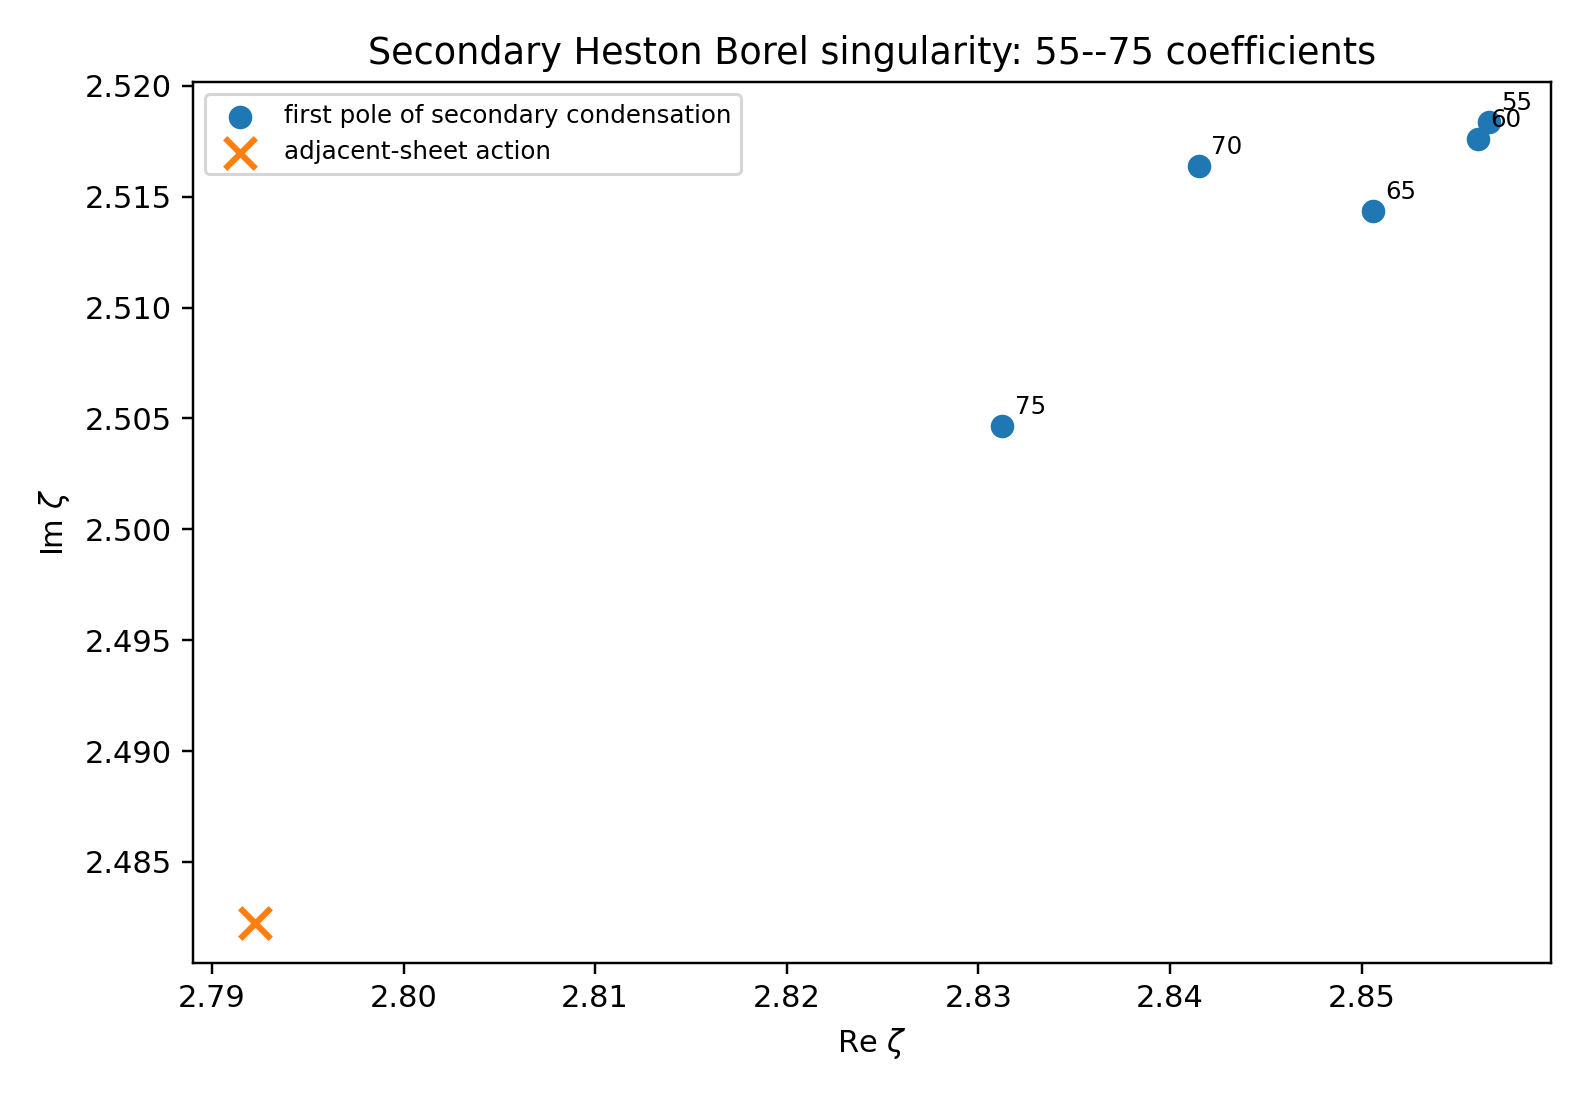
\includegraphics[width=0.82\textwidth]{../figures/heston_secondary_borel_search.png}
\caption{Extended secondary Heston Borel-plane search after conformal removal of the leading cut. The cross denotes the adjacent-sheet action; circles show the first pole of the secondary Pad\'e condensation from 55 through 75 perturbative coefficients.}
\label{fig:secondaryborel}
\end{figure}

\begin{figure}[H]
\centering
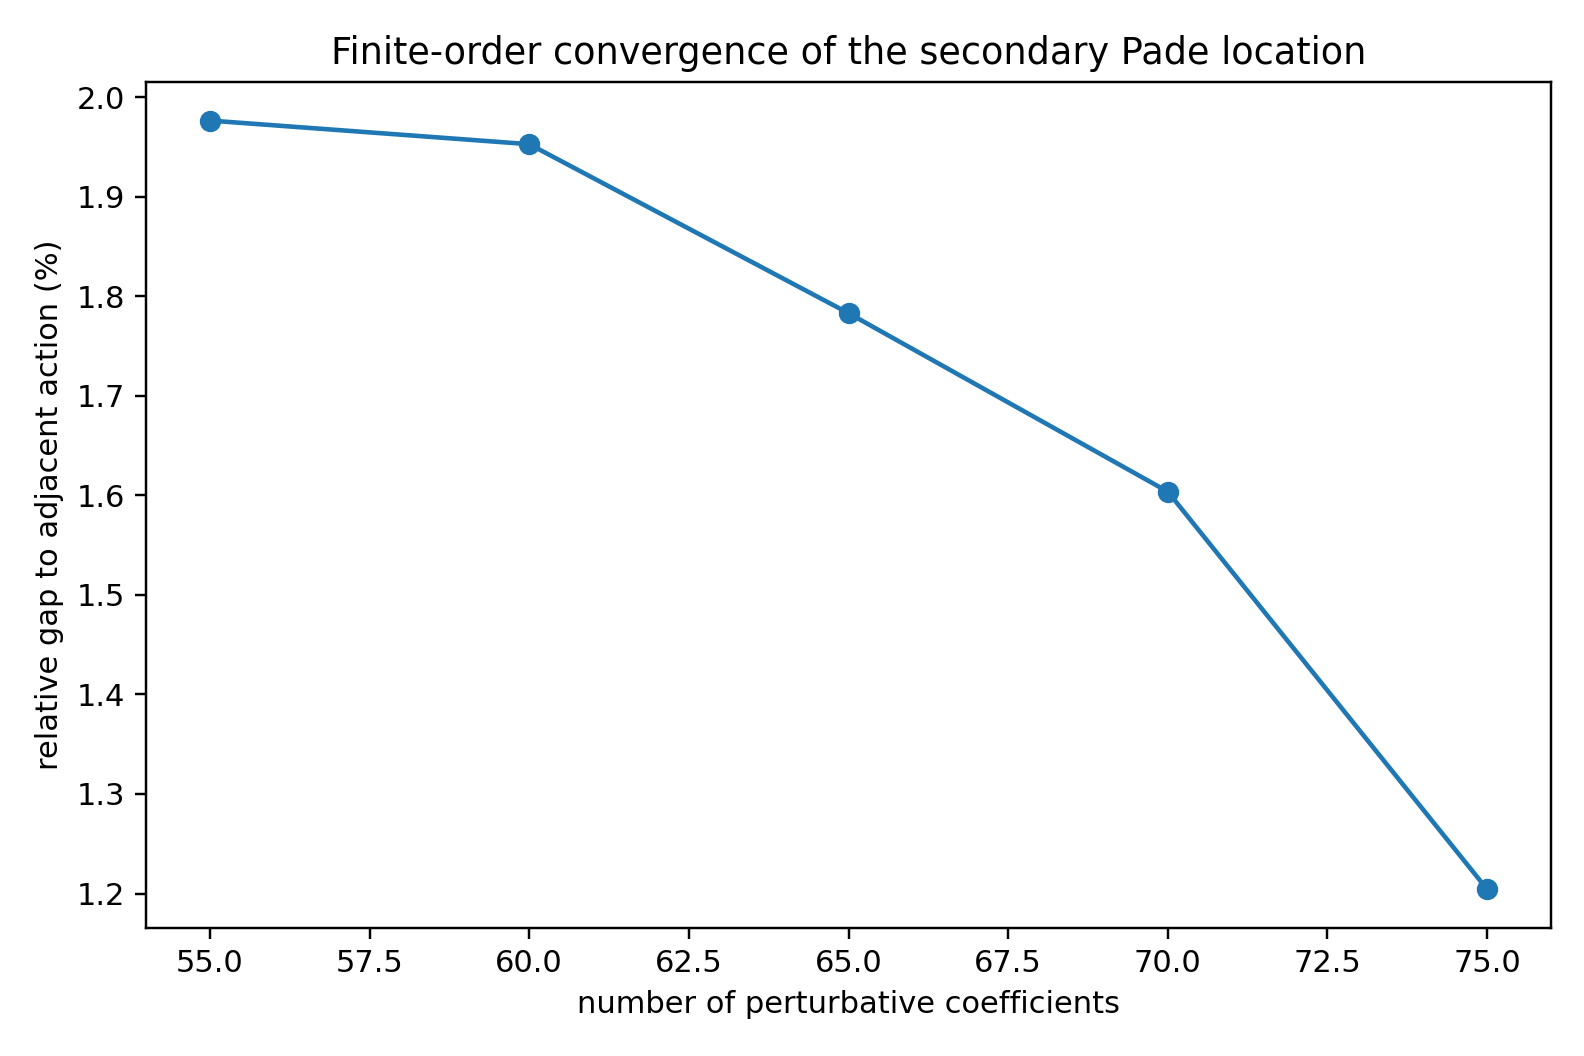
\includegraphics[width=0.82\textwidth]{../figures/heston_secondary_stability.png}
\caption{Relative gap between the first pole of the secondary Pad\'e condensation and the adjacent-sheet action as the perturbative input is increased from 55 to 75 coefficients.}
\label{fig:secondarystability}
\end{figure}

\begin{figure}[H]
\centering
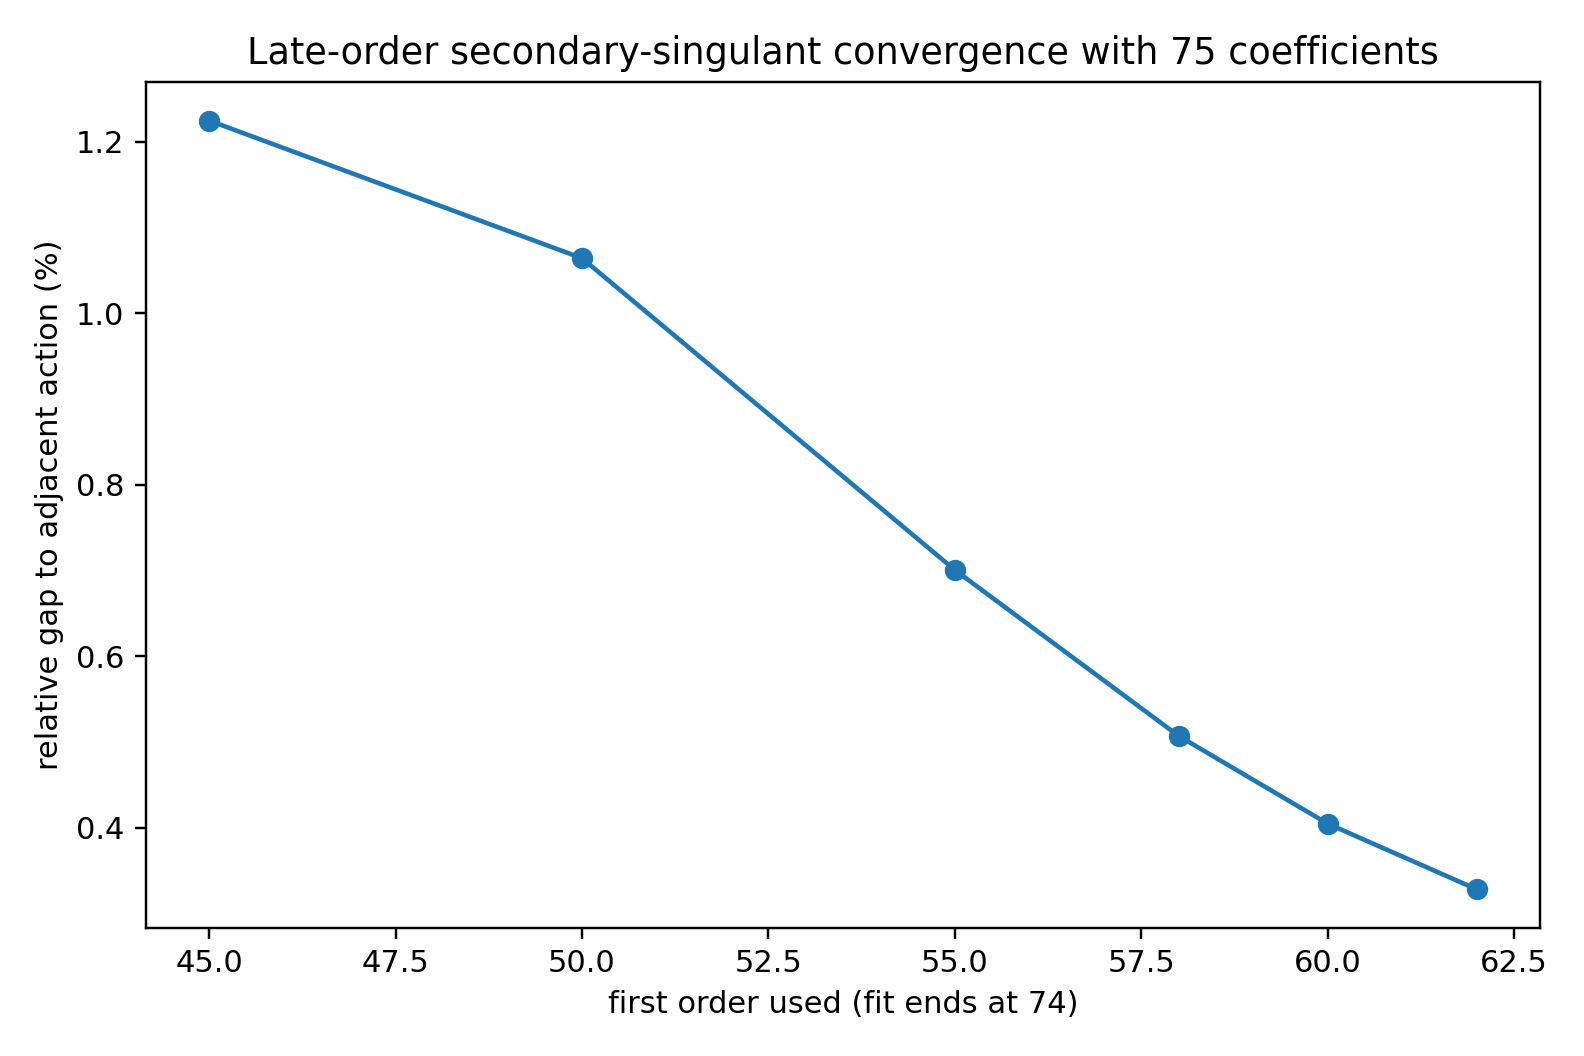
\includegraphics[width=0.82\textwidth]{../figures/heston_secondary_singulant_fit.png}
\caption{Direct logarithmic late-order inference of the secondary singulant using the 75-coefficient conformal-Borel sequence. The fit window is moved to progressively later orders and compared afterward with $\Delta S_1$.}
\label{fig:secondarylatefit}
\end{figure}

\section{Adjacent-saddle fluctuations and effective Stokes data}
A location match is only the first resurgent test. We now ask whether the \emph{local fluctuation sector} around $p_1$ also reproduces the phase and strength of the late coefficients.

Let
\begin{equation}
 \lambda_1=\Lambda''(p_1)=-0.682102187389,
 \qquad
 a_1=\sqrt{-\frac{1}{\lambda_1}}=1.210807992003.
\end{equation}
The local steepest-descent coordinate is
\begin{equation}
 p=p_1+a_1\sqrt\varepsilon\,z,
\end{equation}
for which the quadratic exponent is $-z^2/2$. The adjacent contribution has the formal form
\begin{equation}
 F^{(1)}_\varepsilon
 \sim C_1\sqrt\varepsilon\,
 \e^{\PhiH_1(p_1)/\varepsilon}
 \sum_{n\ge0}d_n\varepsilon^n,
 \qquad
 C_1=\frac{\ii a_1}{p_1\sqrt{2\pi}}.
 \label{eq:adjsector}
\end{equation}
Relative to the physical leading prefactor
\begin{equation}
 C_0=-\frac{1}{p_\star\sqrt{2\pi\Lambda''(p_\star)}},
\end{equation}
we find
\begin{equation}
 \frac{C_1}{C_0}=-0.169547214520\,\ii.
 \label{eq:prefactorratio}
\end{equation}
The first adjacent fluctuation coefficients are
\begin{align}
 d_0&=1,\nonumber\\
 d_1&=0.279264491412,\nonumber\\
 d_2&=-0.006557981878,\nonumber\\
 d_3&=0.114851104087,\nonumber\\
 d_4&=0.224318685187,\nonumber\\
 d_5&=0.493473124613.
 \label{eq:adjcoeffs}
\end{align}
These numbers are obtained by the same Gaussian-moment algebra used at the physical saddle, but with the adjacent steepest-descent direction $a_1$.

For two nondegenerate one-dimensional saddle sectors, the local resurgent relation is expected to be logarithmic. In our normalization we write the singular part of the conformally mapped physical Borel transform as
\begin{equation}
 \widetilde{\calB}_0(w)
 \sim K\,
 \calB_1\!\left(\zeta(w)-\Delta S_1\right)
 \log\!\left(1-\frac{w}{w_1}\right)
 +\overline{K\,
 \calB_1\!\left(\zeta(w)-\Delta S_1\right)
 \log\!\left(1-\frac{w}{w_1}\right)}
 +\text{analytic terms},
 \label{eq:stokeslocal}
\end{equation}
where $\calB_1(t)=\sum d_n t^n/n!$ and $w_1=w(\Delta S_1)$. We define the effective Stokes multiplier by
\begin{equation}
 K=\frac{S_{\rm eff}}{2\pi\ii}\frac{C_1}{C_0}.
 \label{eq:seffdef}
\end{equation}
The qualifier ``effective'' is intentional: a convention-independent Stokes constant would ultimately be fixed by a direct lateral-discontinuity or thimble analysis. Equation~\eqref{eq:seffdef} is the normalization used by the present numerical test.

Expanding \eqref{eq:stokeslocal} about $w=0$ gives an explicit model
\begin{equation}
 b_n^{\rm model}=2\Re(K f_n),
 \label{eq:bnmodel}
\end{equation}
where the $f_n$ are completely determined by $\Delta S_1$, the conformal map and the adjacent coefficients $d_n$. Retaining $d_0,d_1,d_2$ and fitting only the single complex number $K$ over orders 40--59 gives
\begin{equation}
 \boxed{S_{\rm eff}=-0.975897975-0.034122821\,\ii},
 \label{eq:stokesfit}
\end{equation}
with weighted normalized RMS error
\begin{equation}
 \boxed{0.979\%}.
\end{equation}
The value is order one, predominantly real and numerically close to $-1$, as one might expect for a simple saddle connection, but the finite-order data do not justify imposing an exact integer value.

We also perform a genuine holdout test. Fitting $K$ only on orders 40--49 gives
\begin{equation}
 S_{\rm eff}^{\rm train}=-0.979771672-0.039813385\,\ii.
\end{equation}
Without refitting any parameter, this model predicts the unseen orders 50--59 with normalized RMS error
\begin{equation}
 \boxed{1.587\%}.
 \label{eq:holdouterror}
\end{equation}
Thus the adjacent sector reproduces not merely the approximate location of a Borel feature but also the oscillatory phase and amplitude pattern of later perturbative coefficients. Extending the physical series to 75 coefficients and using the later window 60--74 gives the independent cross-check
\begin{equation}
 S_{\rm eff}^{(60:74)}=-0.990549143+0.008669157\,\ii,
 \qquad {\rm NRMSE}=0.417\%.
 \label{eq:stokesfit75}
\end{equation}
The drift toward the negative real axis is consistent with the direct lateral value derived below.

\begin{figure}[H]
\centering
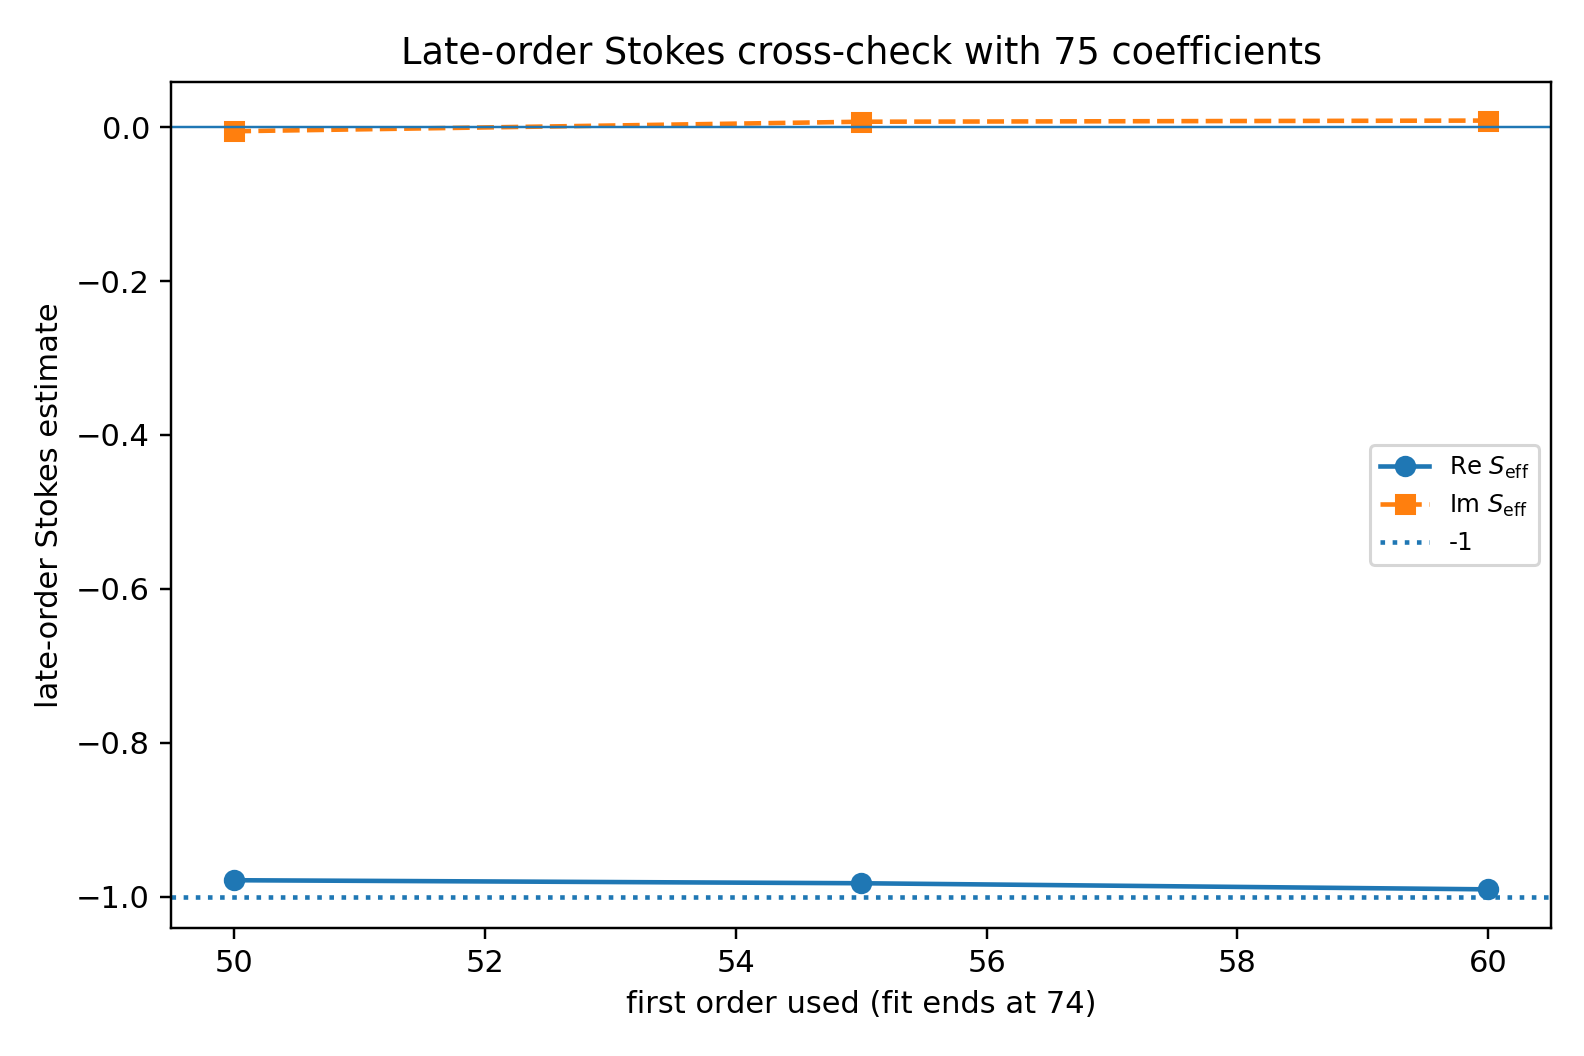
\includegraphics[width=0.82\textwidth]{../figures/heston_stokes_multiplier.png}
\caption{Late-order Stokes cross-check using the 75-coefficient sequence. The real part approaches $-1$ and the residual imaginary part is small as the fit window is moved to later orders.}
\label{fig:stokesmultiplier}
\end{figure}

\begin{figure}[H]
\centering
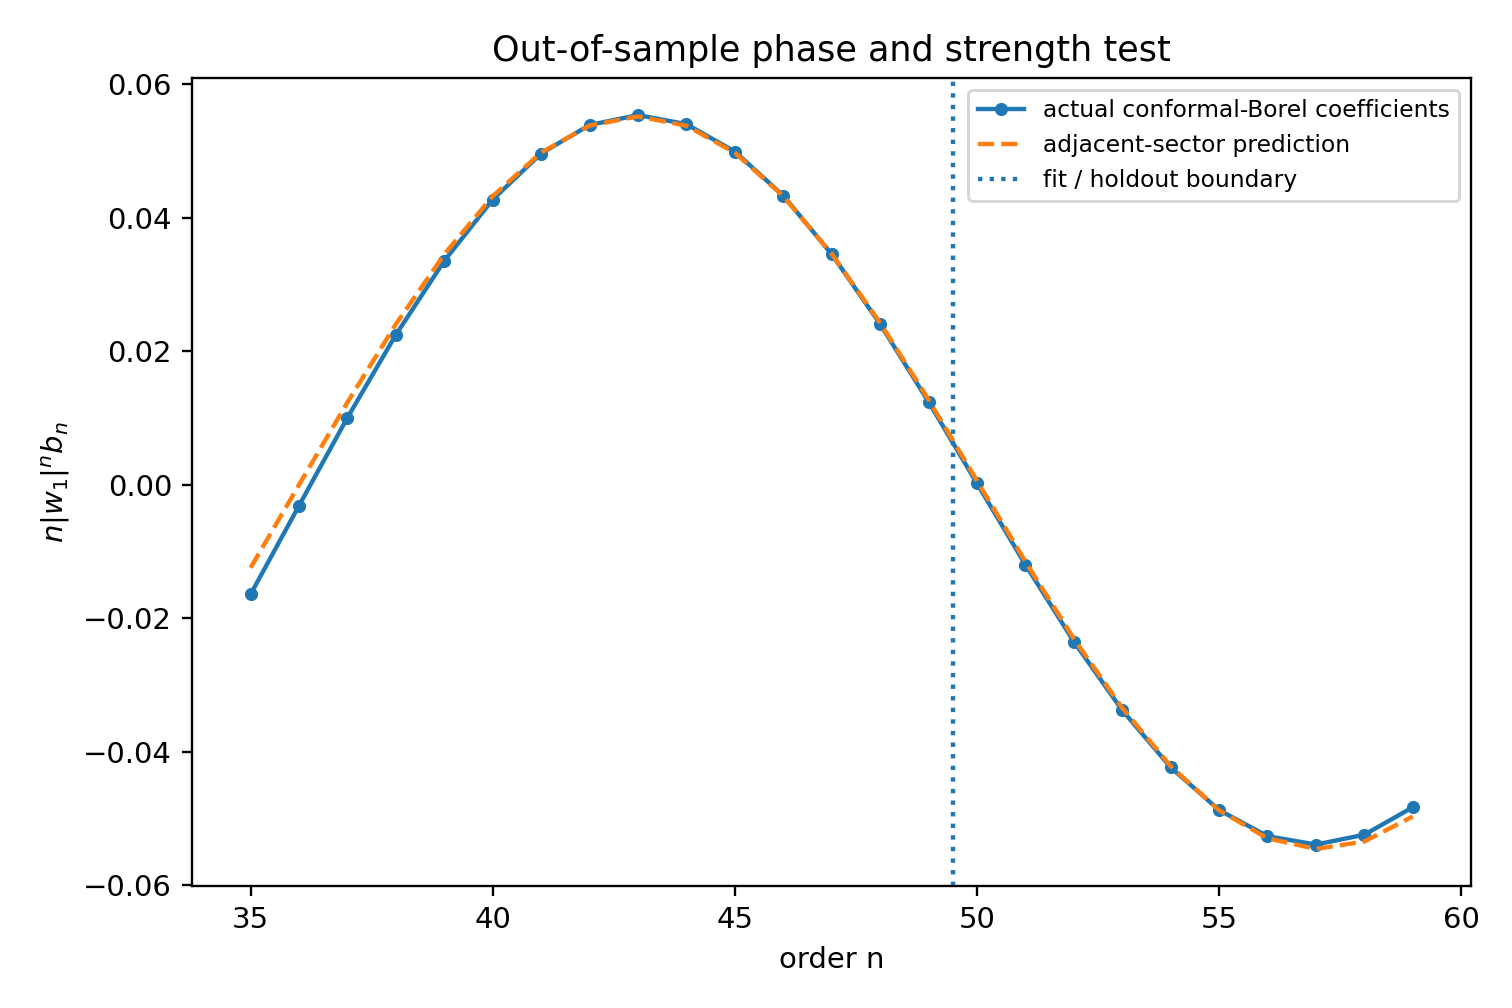
\includegraphics[width=0.82\textwidth]{../figures/heston_secondary_coefficient_prediction.png}
\caption{Normalized conformal-Borel coefficients and the adjacent-sector prediction. The complex branch strength is fitted only through order 49; orders 50--59 form the holdout region.}
\label{fig:holdout}
\end{figure}

\subsection{Interpretation of the secondary result}
Before the direct discontinuity calculation, the secondary evidence already consisted of four mutually consistent ingredients:
\begin{enumerate}
 \item the affine transform has a well-defined stationary point beyond the first negative moment pole;
 \item its imaginary singulant is fixed exactly by logarithmic monodromy;
 \item the 75-coefficient late-order location diagnostic lies within $0.33\%$ of the independently calculated singulant;
 \item the local fluctuation series around that saddle reproduces the phase and amplitude pattern of late perturbative coefficients with an order-one connection coefficient close to $-1$.
\end{enumerate}
The remaining question is whether the same connection strength is obtained by crossing the Borel singularity directly, without fitting the late coefficients. This is the purpose of the next section.


\section{Direct lateral discontinuity and a hyperasymptotic jump test}
The preceding extraction of $S_{\rm eff}$ still used late perturbative coefficients in a fit. We now compute the same connection coefficient by a different operation: analytic continuation of the Borel transform across the secondary Stokes direction.

Let
\begin{equation}
 \vartheta_1=\arg \Delta S_1,
 \qquad
 \varepsilon=r\,\e^{\ii\vartheta_1},
 \qquad r>0.
\end{equation}
For the exact Borel transform, resurgence predicts
\begin{equation}
 \operatorname{Disc}_{\vartheta_1}\Phi_0(\varepsilon)
 =S_{01}\frac{C_1}{C_0}
 \e^{-\Delta S_1/\varepsilon}
 \mathcal S_{\vartheta_1}\Phi_1(\varepsilon),
 \label{eq:lateralresurgence}
\end{equation}
where $\Phi_1(\varepsilon)=\sum_{n\ge0}d_n\varepsilon^n$ is the adjacent fluctuation sector and the convention for $C_1/C_0$ is that of Eq.~\eqref{eq:prefactorratio}.

At finite order the conformal-Pad\'e approximant replaces the logarithmic cut by simple poles $\zeta_j$ with residues $r_j$. When the lateral contour is moved through that pole string, Cauchy's theorem gives
\begin{equation}
 \operatorname{Disc}_{\vartheta_1}\Phi_0(\varepsilon)
 \simeq \frac{2\pi\ii}{\varepsilon}
 \sum_{j\in\mathcal C_1}
 r_j\,\e^{-\zeta_j/\varepsilon},
 \label{eq:padejump}
\end{equation}
where $\mathcal C_1$ denotes the pole condensation issuing from the first secondary singularity. No branch-strength or Stokes parameter is fitted in Eq.~\eqref{eq:padejump}. The residues are obtained directly from the rational approximant, including the Jacobian from the conformal map.

Using 75 physical coefficients, the first poles in $\mathcal C_1$ begin at
\begin{equation}
 \zeta_1^{(75)}=2.831243366402+2.504669377762\,\ii,
\end{equation}
and then continue away from the branch point as expected for a finite rational representation of a cut. Dividing the residue jump by the independently computed adjacent sector according to Eq.~\eqref{eq:lateralresurgence} gives
\begin{equation}
 \boxed{S_{\rm lateral}=-0.998565810+0.001484197\,\ii}
 \qquad (r=0.18,N=75).
 \label{eq:lateralstokes}
\end{equation}
Its distance from $-1$ is $2.06\times10^{-3}$, or $0.206\%$. At the same $r$, changing the input order from $N=55$ to $N=75$ keeps the result within roughly three parts in $10^{-3}$ of $-1$. Thus the value is not generated by one exceptional Pad\'e approximant.

\begin{figure}[H]
\centering
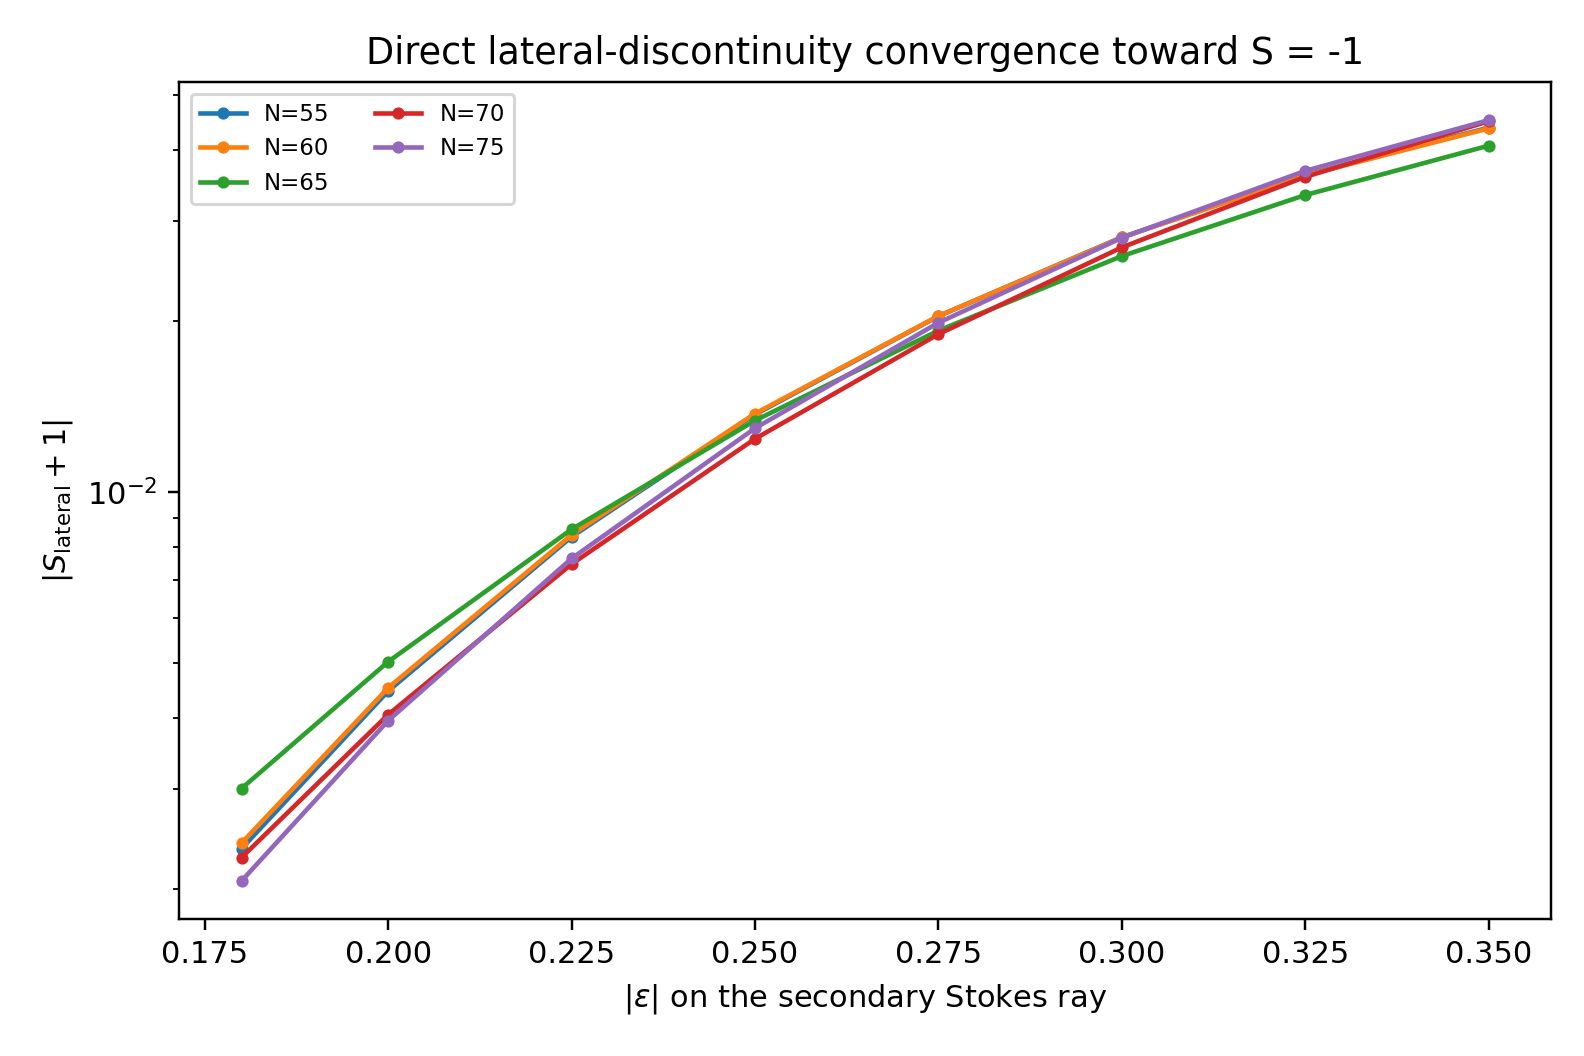
\includegraphics[width=0.82\textwidth]{../figures/heston_lateral_stokes.png}
\caption{Distance of the direct lateral Pad\'e-residue Stokes estimate from $S=-1$. No late-order branch-strength fit is used; the estimates from 55--75 coefficients agree at the few-$10^{-3}$ level in the controlled small-$|\varepsilon|$ regime.}
\label{fig:lateralstokes}
\end{figure}

The same calculation yields a first hyperasymptotic consistency test. Define the reduced discontinuity assuming the simple connection coefficient $S_{01}=-1$,
\begin{equation}
 R_1(\varepsilon)
 =-\frac{\operatorname{Disc}_{\vartheta_1}\Phi_0(\varepsilon)}
 {(C_1/C_0)\e^{-\Delta S_1/\varepsilon}}.
 \label{eq:reducedjump}
\end{equation}
Equation~\eqref{eq:lateralresurgence} predicts $R_1\sim\Phi_1$. At $r=0.18$, using only $d_0=1$ gives a $4.61\%$ relative error, while including the computed adjacent fluctuations through $d_9$ reduces the error to
\begin{equation}
 \boxed{0.207\%}.
 \label{eq:hypererror}
\end{equation}
The improvement is asymptotic rather than monotonic at larger $r$, as expected from the eventual factorial growth of the adjacent series.

\begin{figure}[H]
\centering
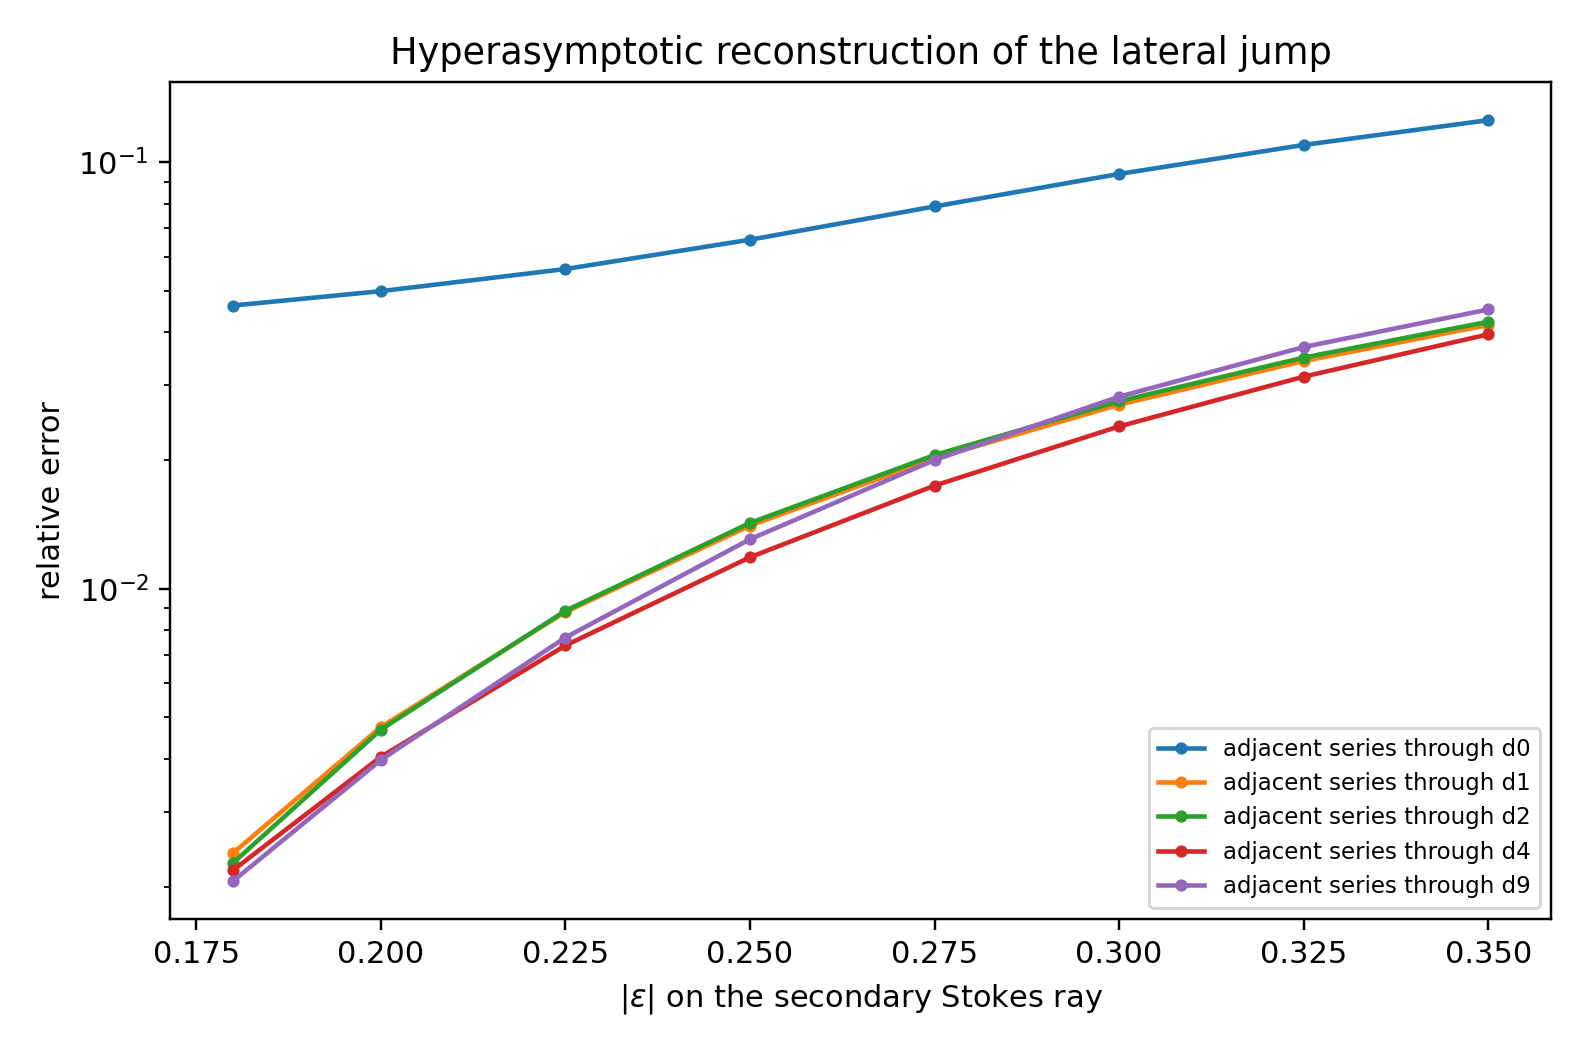
\includegraphics[width=0.82\textwidth]{../figures/heston_hyperasymptotic_jump.png}
\caption{Hyperasymptotic reconstruction of the independently computed lateral jump with successive adjacent-sector fluctuations. The strongest improvement occurs in the small-$|\varepsilon|$ regime where the saddle expansion is controlled.}
\label{fig:hyperjump}
\end{figure}

\begin{figure}[H]
\centering
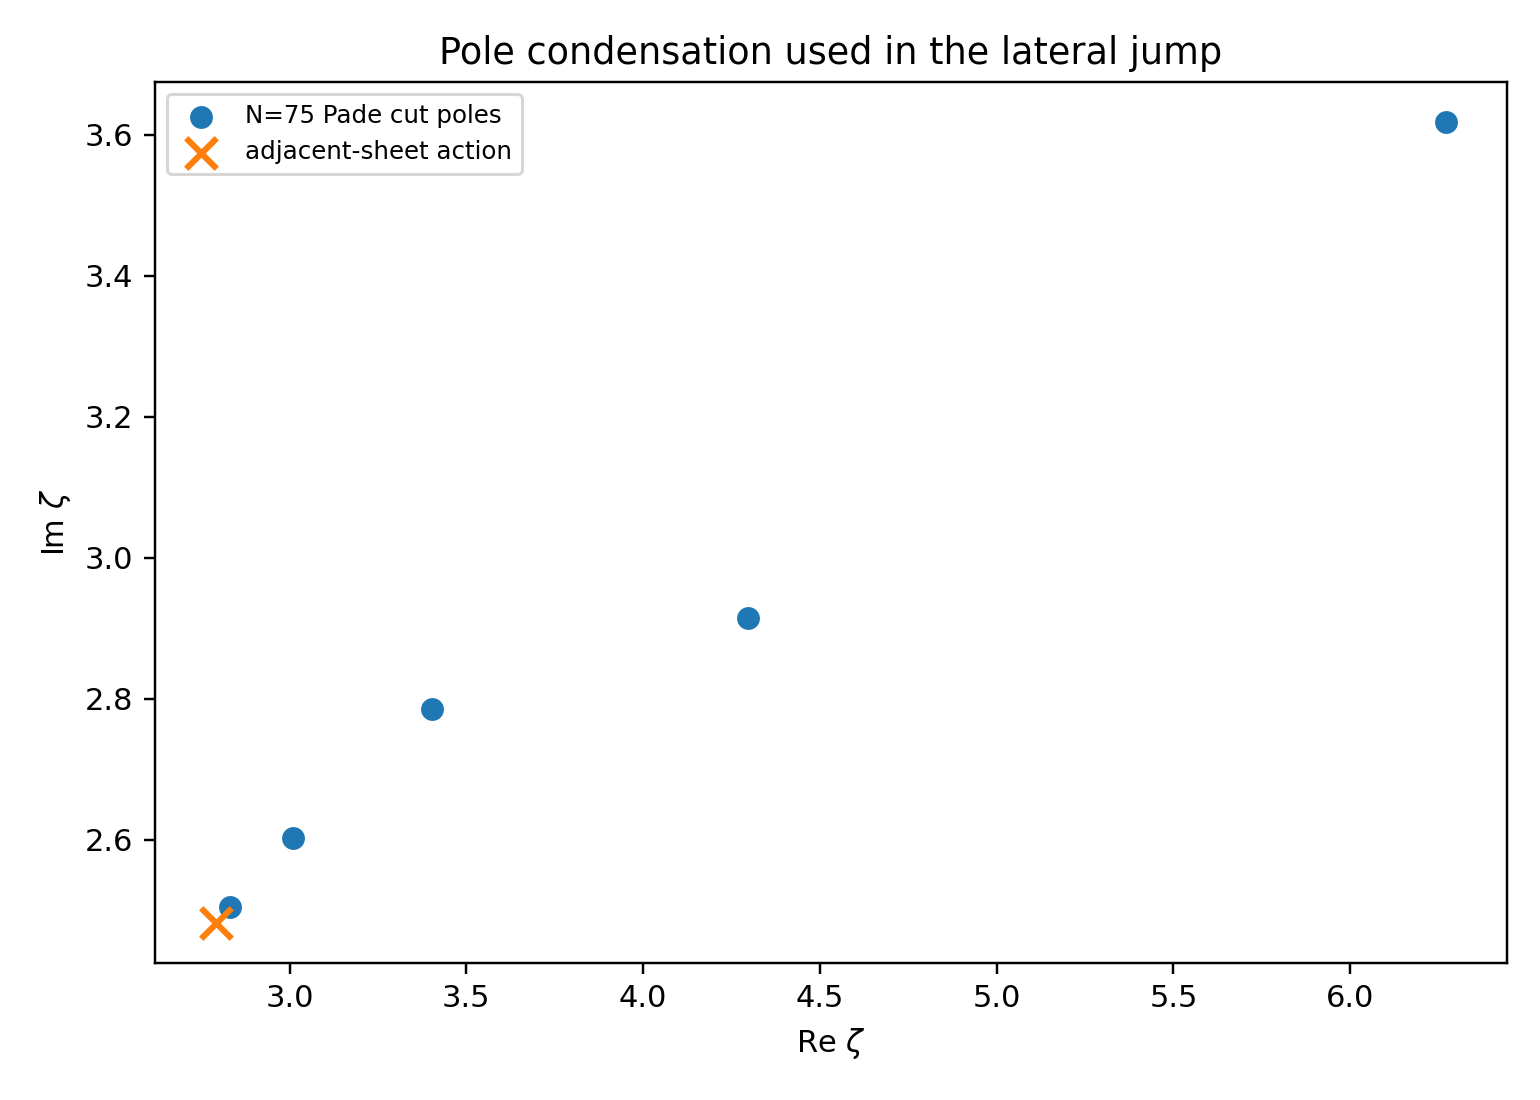
\includegraphics[width=0.72\textwidth]{../figures/heston_lateral_pade_chain.png}
\caption{The finite-order Pad\'e pole condensation used in the residue evaluation of the secondary lateral discontinuity, together with the independently computed adjacent-sheet action.}
\label{fig:lateralchain}
\end{figure}

This direct discontinuity calculation changes the status of the secondary test. The Stokes strength is no longer inferred only from coefficient fitting: two numerically distinct procedures---late-order resurgence and a lateral Borel residue calculation---both select a multiplier close to $-1$, while the adjacent fluctuation sector reconstructs the subleading structure of the jump itself. The remaining limitation at this stage is to explain the near-integer connection coefficient geometrically.

\section{Picard--Lefschetz wall crossing and the sign of the Stokes integer}
We now complexify the one-dimensional affine inversion and study its steepest-descent geometry directly. This is the finite-dimensional Picard--Lefschetz setting developed for saddle integrals by Pham and used broadly in modern complexified path integrals \citep{pham1983,witten2011}. Write
\begin{equation}
 h_{\vartheta}(p)=\e^{-\ii\vartheta}\Phi(p),
 \qquad \Phi(p)=\Lambda(p)-p x_\star,
 \label{eq:rotatedphase}
\end{equation}
where only the phase $\vartheta=\arg\varepsilon$ matters for the geometry. A positive rescaling of $|\varepsilon|$ merely reparametrises flow time. The upward and downward flows are
\begin{equation}
 \frac{\dd p}{\dd\tau}=+\overline{h'_{\vartheta}(p)},
 \qquad
 \frac{\dd p}{\dd\tau}=-\overline{h'_{\vartheta}(p)},
 \label{eq:plflows}
\end{equation}
respectively. Along either flow $\operatorname{Im}h_{\vartheta}$ is constant, while $\operatorname{Re}h_{\vartheta}$ increases on the upward cycle and decreases on the downward thimble.

For a nondegenerate saddle $p_\sigma$ with curvature $\Lambda''(p_\sigma)$, the local upward directions obey
\begin{equation}
 \alpha_{\rm up}=-\frac12\arg\!\left[\Lambda''(p_\sigma)\e^{-\ii\vartheta}\right]\quad (\mathrm{mod}\;\pi),
 \label{eq:updirection}
\end{equation}
with the downward directions rotated by $\pi/2$. We denote the downward thimble through $p_\sigma$ by $\mathcal J_\sigma$ and its upward dual cycle by $\mathcal K_\sigma$. For an upward-oriented Bromwich line $\Gamma_B$ inside the moment strip,
\begin{equation}
 \Gamma_B=\sum_\sigma n_\sigma\mathcal J_\sigma,
 \qquad
 n_\sigma=\langle\Gamma_B,\mathcal K_\sigma\rangle,
 \label{eq:thimbledecomp}
\end{equation}
where the coefficients are oriented intersection numbers.

The secondary Stokes angle is fixed without fitting:
\begin{equation}
 \boxed{\vartheta_1=\arg\Delta S_1=0.726693312478\ \mathrm{rad}.}
 \label{eq:stokesangle}
\end{equation}
At this angle the two saddles have equal phase,
\begin{equation}
 \operatorname{Im}\!\left[\e^{-\ii\vartheta_1}\Phi(p_1)\right]
 =\operatorname{Im}\!\left[\e^{-\ii\vartheta_1}\Phi(p_\star)\right],
\end{equation}
and one branch of the upward cycle $\mathcal K_1$ from $p_1$ approaches the physical saddle. Numerically integrating Eq.~\eqref{eq:plflows} gives a minimum separation $|p-p_\star|=7.96\times10^{-5}$ at the finite integration cutoff, with continued convergence as the flow time is extended. This is the expected heteroclinic connection at the Stokes wall.

To determine the integer and its sign we move slightly off the wall and use the admissible Bromwich line $\operatorname{Re}p=-1$. For phase offsets
\begin{equation}
 \delta\vartheta\in\{-0.05,-0.04,\ldots,-0.01\},
\end{equation}
the continued branch has no intersection with $\Gamma_B$ and hence
\begin{equation}
 \langle\Gamma_B,\mathcal K_1\rangle=0.
\end{equation}
For every tested
\begin{equation}
 \delta\vartheta\in\{0.01,0.02,\ldots,0.05\},
\end{equation}
the same branch crosses $\Gamma_B$ exactly once. The crossing is from left to right while $\Gamma_B$ is oriented upward. With the plane orientation $(\operatorname{Re}p,\operatorname{Im}p)$,
\begin{equation}
 \operatorname{sgn}\det(t_{\Gamma_B},t_{\mathcal K_1})=-1,
\end{equation}
so the intersection number above the wall is
\begin{equation}
 \boxed{\langle\Gamma_B,\mathcal K_1\rangle=-1.}
 \label{eq:intersectionminusone}
\end{equation}
Thus the thimble decomposition jumps by one oppositely oriented copy of the adjacent thimble,
\begin{equation}
 \Gamma_B^{+}=\Gamma_B^{-}-\mathcal J_1,
 \label{eq:pljump}
\end{equation}
and, in the normalization of Eq.~\eqref{eq:lateralresurgence}, the Picard--Lefschetz connection integer is
\begin{equation}
 \boxed{S_{01}^{\rm PL}=-1.}
 \label{eq:stokesexactgeom}
\end{equation}
This agrees with the completely independent Borel-residue value
\begin{equation}
 S_{\rm lateral}=-0.998565810+0.001484197\,\ii
\end{equation}
to $0.206\%$.

\begin{figure}[H]
\centering
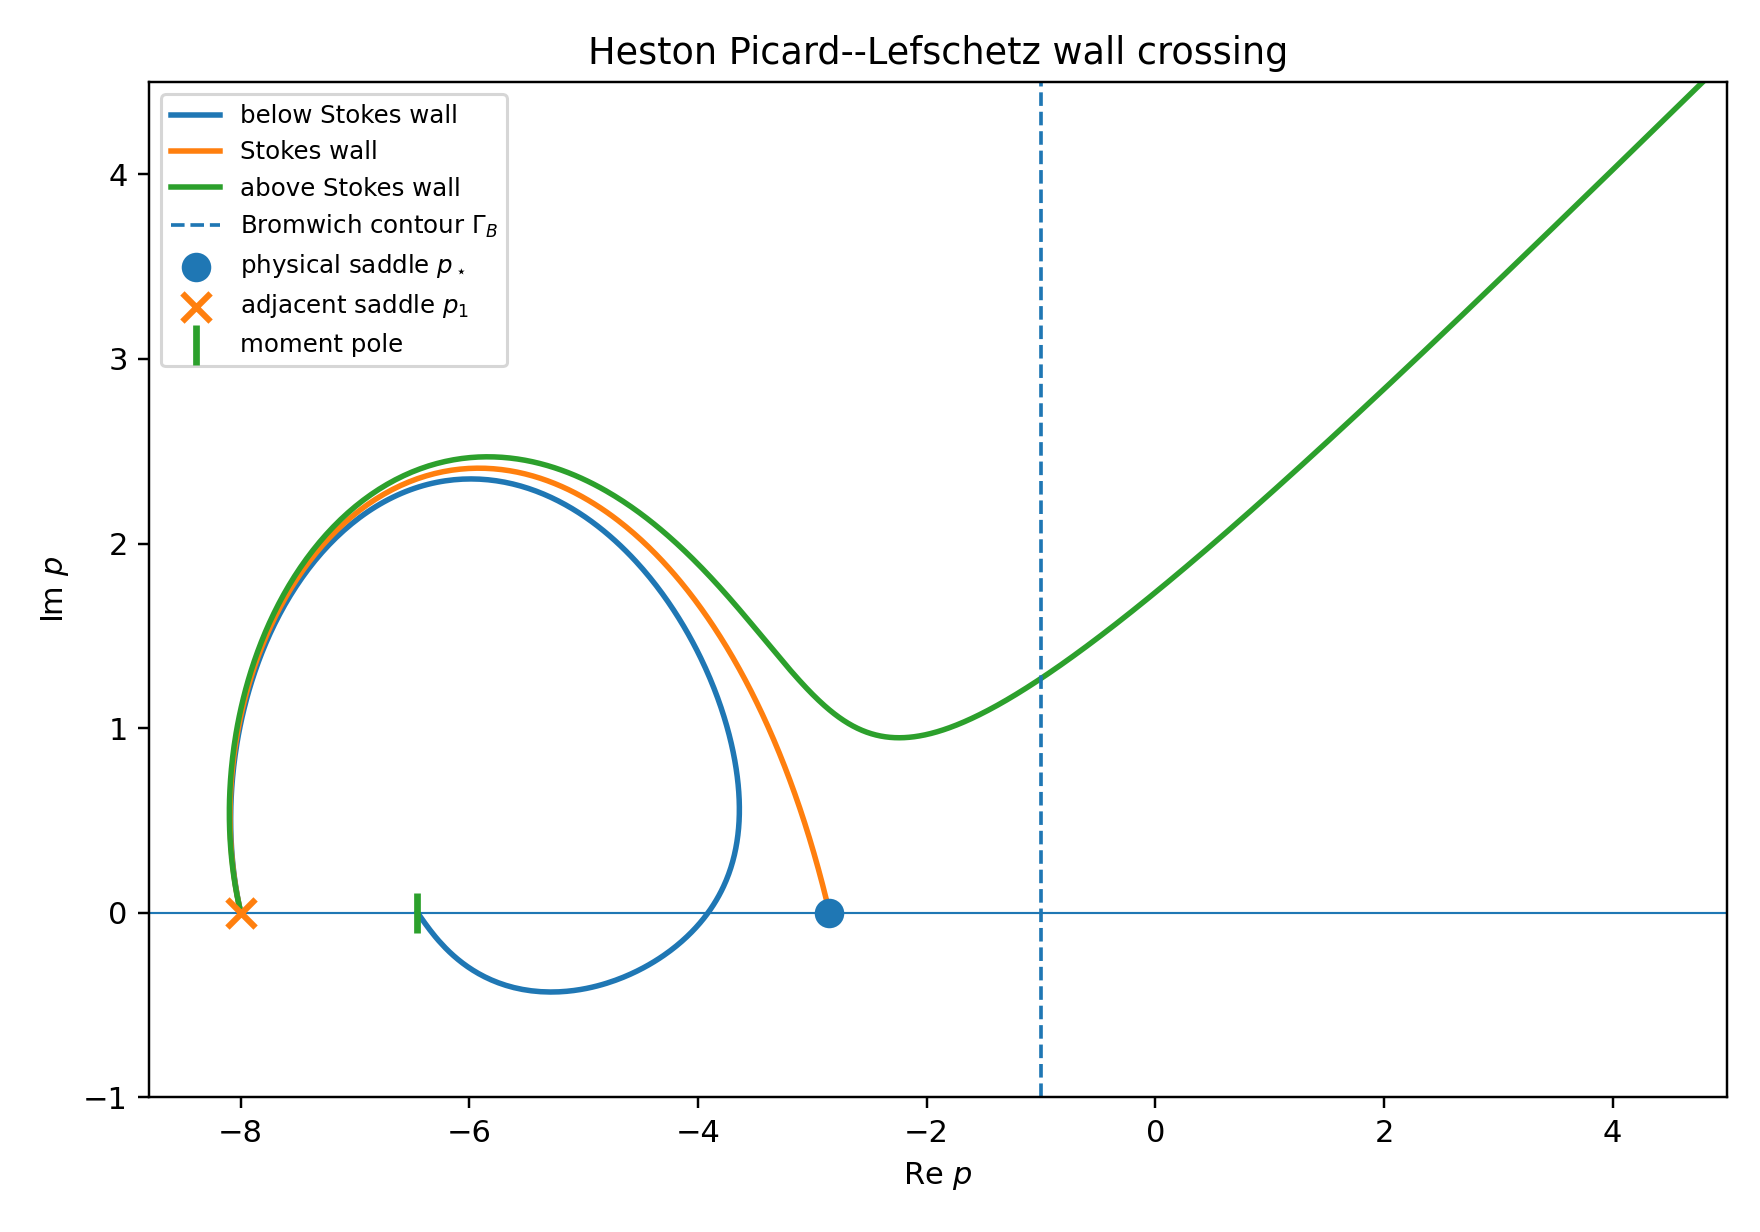
\includegraphics[width=0.88\textwidth]{../figures/heston_thimble_wall_crossing.png}
\caption{Complex-$p$ Picard--Lefschetz geometry around the secondary Stokes wall. Below the wall the selected upward branch does not meet the Bromwich contour. On the wall it forms a heteroclinic connection from the adjacent saddle to the physical saddle. Above the wall it crosses the Bromwich contour once.}
\label{fig:thimblewall}
\end{figure}

\begin{figure}[H]
\centering
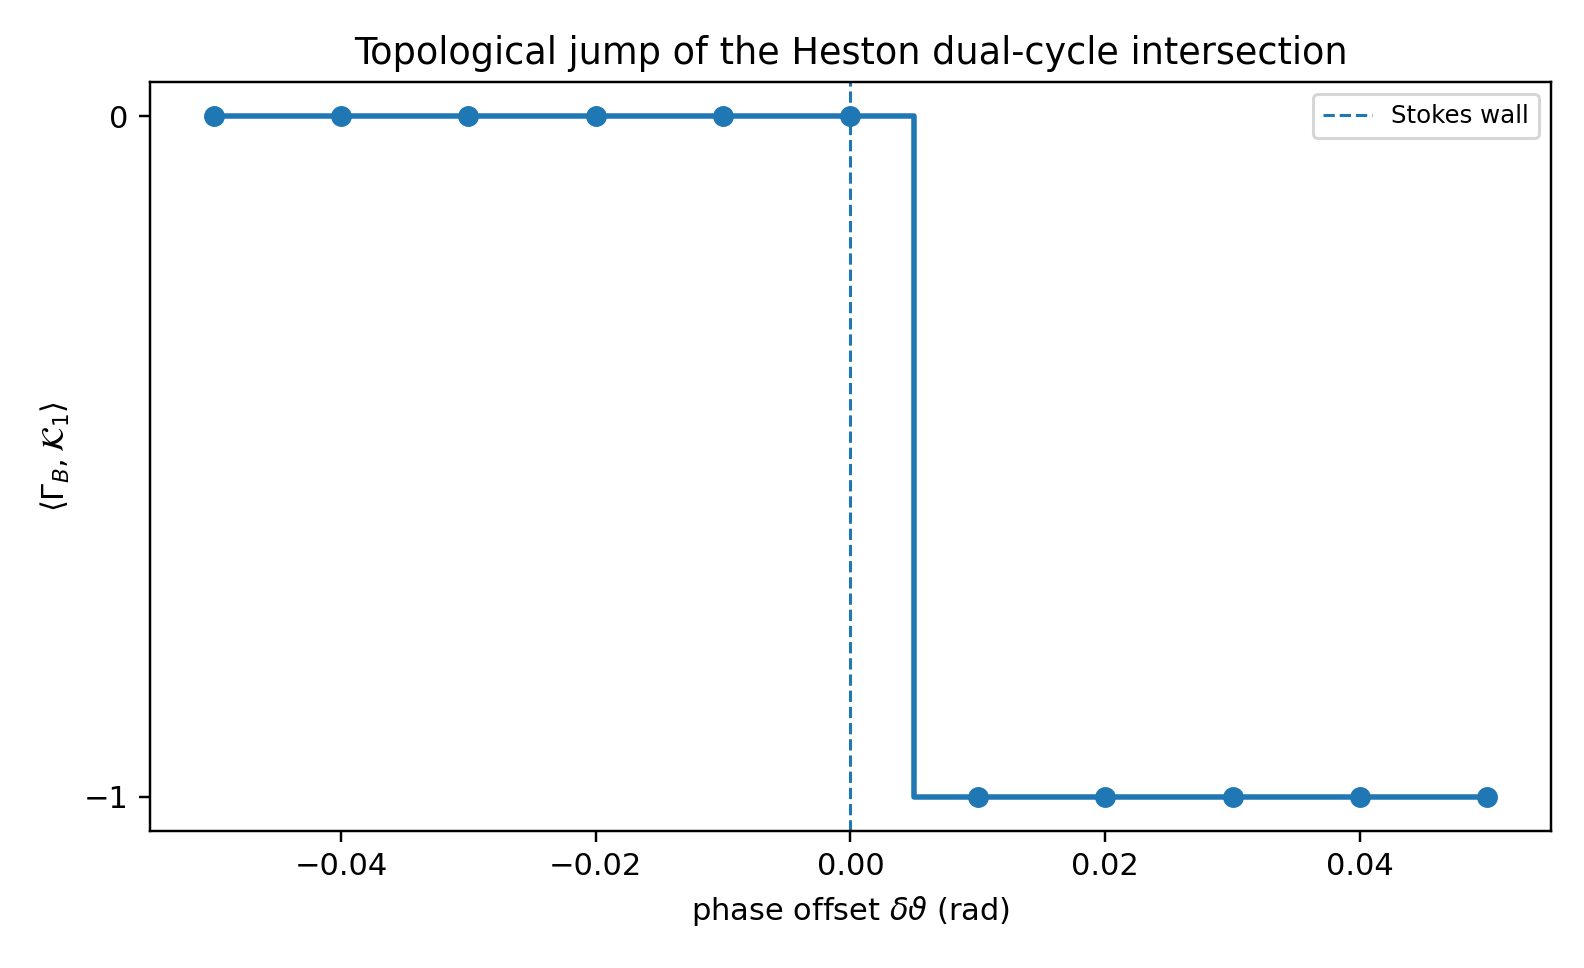
\includegraphics[width=0.72\textwidth]{../figures/heston_thimble_intersection_jump.png}
\caption{The oriented dual-cycle intersection number is topologically stable away from the wall and jumps from $0$ to $-1$ as $\arg\varepsilon$ crosses $\vartheta_1$.}
\label{fig:intersectionjump}
\end{figure}

\begin{figure}[H]
\centering
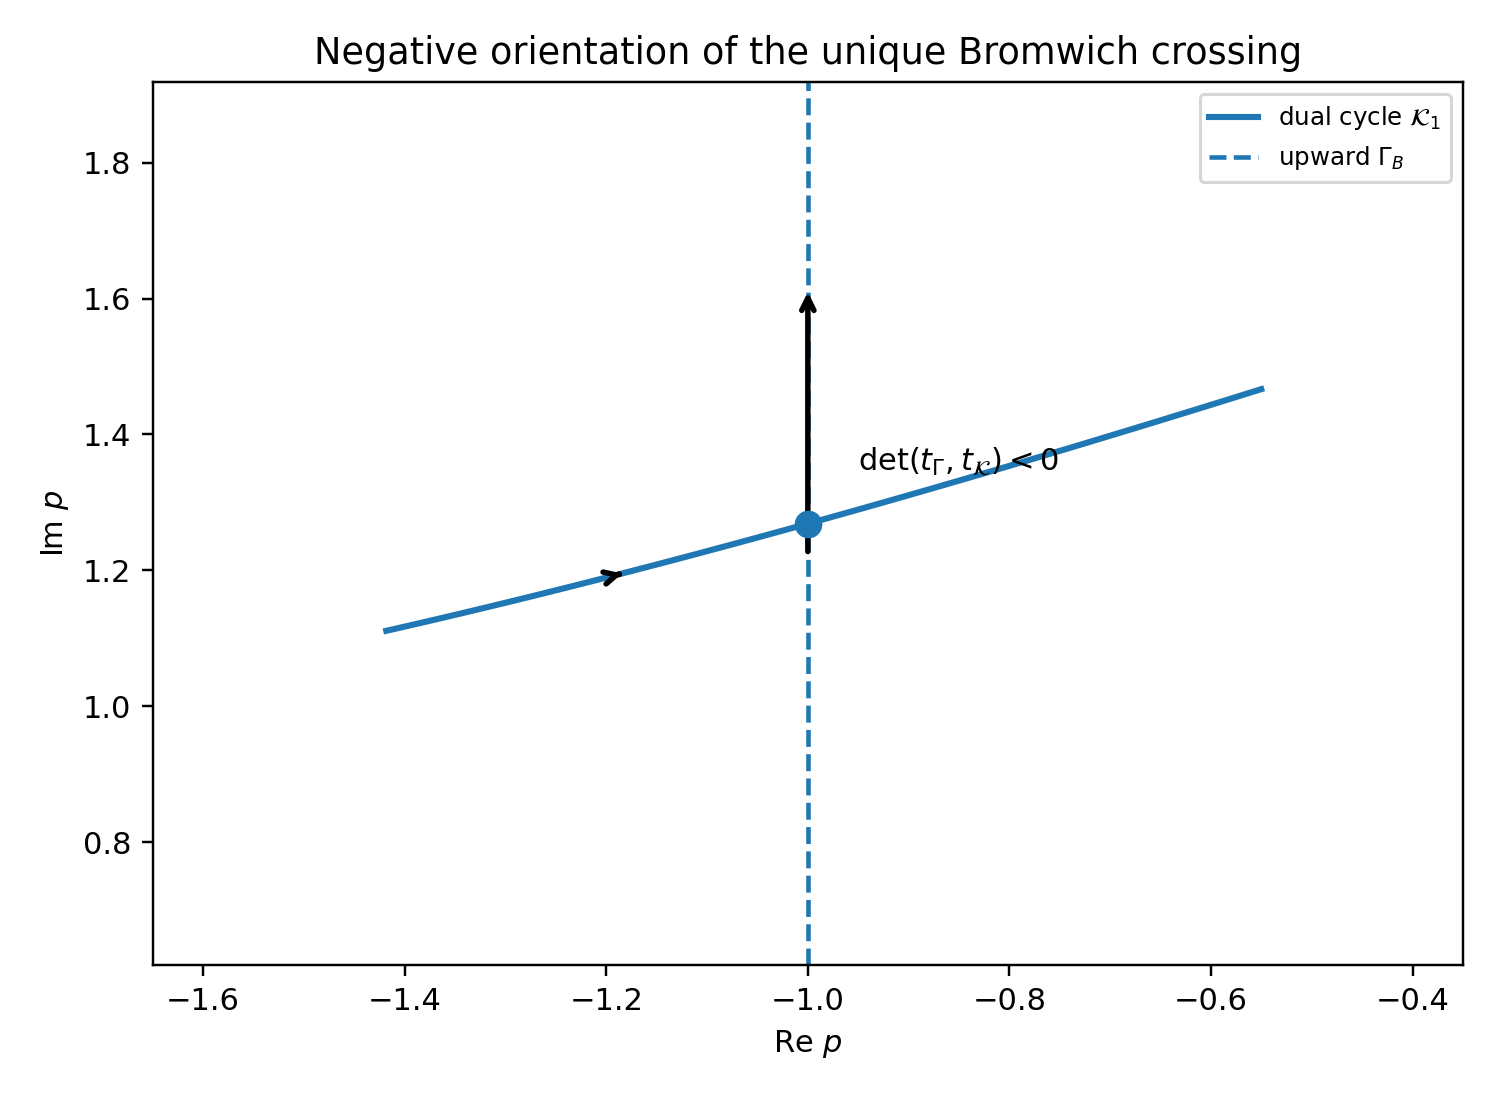
\includegraphics[width=0.72\textwidth]{../figures/heston_thimble_orientation.png}
\caption{Orientation of the unique crossing just above the wall. The Bromwich contour points upward and the dual cycle crosses from left to right, giving $\det(t_{\Gamma_B},t_{\mathcal K_1})<0$ and therefore intersection number $-1$.}
\label{fig:orientation}
\end{figure}

The result should be interpreted with the appropriate level of rigor. The integer itself is topological once the global flow connectivity is fixed, and its value is stable over the tested phase offsets. However, the present work establishes that connectivity by numerical integration of the complex flow rather than by an analytic global classification of every singularity and end of the Heston Riemann surface. Equation~\eqref{eq:stokesexactgeom} is therefore a geometric/topological result for the benchmark contour supported by reproducible flow computation, not a general theorem for all Heston parameters.

\section{Potential transseries structure}
The natural multi-sector completion suggested by the present calculation is
\begin{align}
 F_\varepsilon(x_\star)
 \sim&\;
 C_0\sqrt\varepsilon\,\e^{-I/\varepsilon}
 \Phi_0(\varepsilon)\nonumber\\
 &+\sigma_1 C_1\sqrt\varepsilon\,
 \e^{-(I+\Delta S_1)/\varepsilon}\Phi_1(\varepsilon)
 +\bar\sigma_1\,\overline{C_1}\sqrt\varepsilon\,
 \e^{-(I+\overline{\Delta S_1})/\varepsilon}
 \overline{\Phi_1(\varepsilon)}+\cdots,
 \label{eq:transseries}
\end{align}
with $\Phi_0=\sum c_n\varepsilon^n$ and $\Phi_1=\sum d_n\varepsilon^n$. Equation~\eqref{eq:transseries} is now supported by location, phase, strength, direct lateral-discontinuity and Picard--Lefschetz wall-crossing tests. For the benchmark contour the dual-cycle calculation fixes the connection integer to $S_{01}=-1$, in agreement with the lateral Borel calculation. The remaining caution is global: the thimble connectivity has been established numerically for this parameter point rather than classified analytically for the full Heston Riemann surface. Thus the equation is a quantitatively and geometrically supported two-sector transseries for this observable, not a theorem about the entire Heston family.

A parameter-dependent change in which complex saddle controls the late terms would produce a Stokes phenomenon in the asymptotic representation. Such a mathematical Stokes transition should not be identified naively with an empirical market ``regime change''; the statement would concern the saddle decomposition of a specified stochastic model.

\section{Why renormalons are not claimed}
The present instanton/singulant structure has a direct stochastic origin: the small-noise path integral carries exponentially small weights $\e^{-A/\varepsilon}$ and the affine inversion has identifiable saddles and singularities. Renormalons are conceptually different. In quantum field theory they are associated with factorial growth generated by integration over hierarchies of scales and with renormalization-group structure. A financial analogue would therefore require a genuine multiscale effective theory with running couplings under temporal or cross-sectional coarse graining. The observation of factorial coefficients or Borel poles in the Heston expansion is not sufficient evidence for a renormalon. Renormalons remain a separate future research question.

\section{Numerical implementation and reproducibility}\label{sec:repro}
The repository is organised as a small research codebase rather than a monolithic notebook. The main ingredients are:
\begin{itemize}
 \item exact affine scaled cumulant generator $\Lambda(p)$;
 \item arbitrary-precision real saddle solving and Cauchy-integral high-order Taylor extraction;
 \item formal Gaussian-moment generation of the fluctuation coefficients;
 \item continuous Freidlin--Wentzell Hamiltonian shooting;
 \item Borel transforms, near-diagonal Pad\'e approximants and Gauss--Laguerre Borel integration;
 \item numerical affine contour inversion for a reference probability;
 \item moment-pole location and adjacent-sheet saddle continuation;
 \item high-precision conformal Borel composition for the secondary search;
 \item adjacent-sheet fluctuation generation, logarithmic late-order fitting and effective Stokes-strength extraction;
 \item complex Picard--Lefschetz flow integration and oriented Bromwich-intersection counting;
 \item parameter continuation, moment-pole tracking, fold detection and anti-Stokes root finding.
\end{itemize}
The current automated suite contains fourteen tests, all passing. The main experiments are reproduced with
\begin{verbatim}
python experiments/run_gaussian_resurgence.py
python experiments/run_quartic_factor_resurgence.py
python experiments/run_heston_resurgence.py
python experiments/run_heston_secondary_resurgence.py
python experiments/run_heston_stokes_resurgence.py
python experiments/run_heston_lateral_resurgence.py --reuse-coefficients
python experiments/run_heston_thimble_geometry.py
python experiments/run_heston_parameter_generalization.py --structural-only
python experiments/run_heston_generalization_summary.py
python experiments/run_heston_resurgent_phase_diagram.py
python experiments/run_heston_uniform_airy_fold.py
python experiments/run_heston_global_phase_portrait.py
\end{verbatim}
The secondary experiments intentionally use arbitrary precision during the conformal composition because ordinary double precision was empirically found to generate catastrophic cancellation at high order. The 75-coefficient physical expansion uses the Cauchy extractor in Eq.~\eqref{eq:cauchytaylor}, which removes the previous high-derivative bottleneck.

\section{Parameter continuation and robustness of the two-sector structure}
\label{sec:generalization}
The benchmark analysis establishes a two-sector relation at one point in parameter space. A stronger question is whether the same analytic and topological structure survives continuous deformations of the Heston parameters. We therefore perform one-parameter continuation in
\begin{equation}
 x_\star\in[-0.35,-0.15],\qquad
 T\in[0.5,2],\qquad
 \rho\in[-0.9,0],\qquad
 \xi\in[0.25,0.8],\qquad
 \kappa\in[0.75,4],
 \label{eq:sweepranges}
\end{equation}
with five points per axis and all other quantities fixed to the benchmark values. The continuation algorithm explicitly locates the first two negative moment poles and selects the first stationary point between them. This prevents a Newton solver from jumping to a more distant logarithmic sheet as maturity or other parameters vary.

\subsection{Exact monodromy under parameter continuation}
For every one of the 25 sweep points the adjacent action satisfies
\begin{equation}
 \boxed{\operatorname{Im}\Delta S_1=2\pi\frac{\kappa\theta}{\xi^2}},
 \label{eq:generalmonodromy}
\end{equation}
with maximum absolute numerical discrepancy below $10^{-14}$. Consequently the imaginary part is independent of $x_\star$, $T$ and $\rho$, while its $\kappa$ and $\xi$ dependence is fixed entirely by the logarithmic monodromy. Figure~\ref{fig:generalmonodromy} shows the observed and predicted values over the complete sweep.

\begin{figure}[H]
\centering
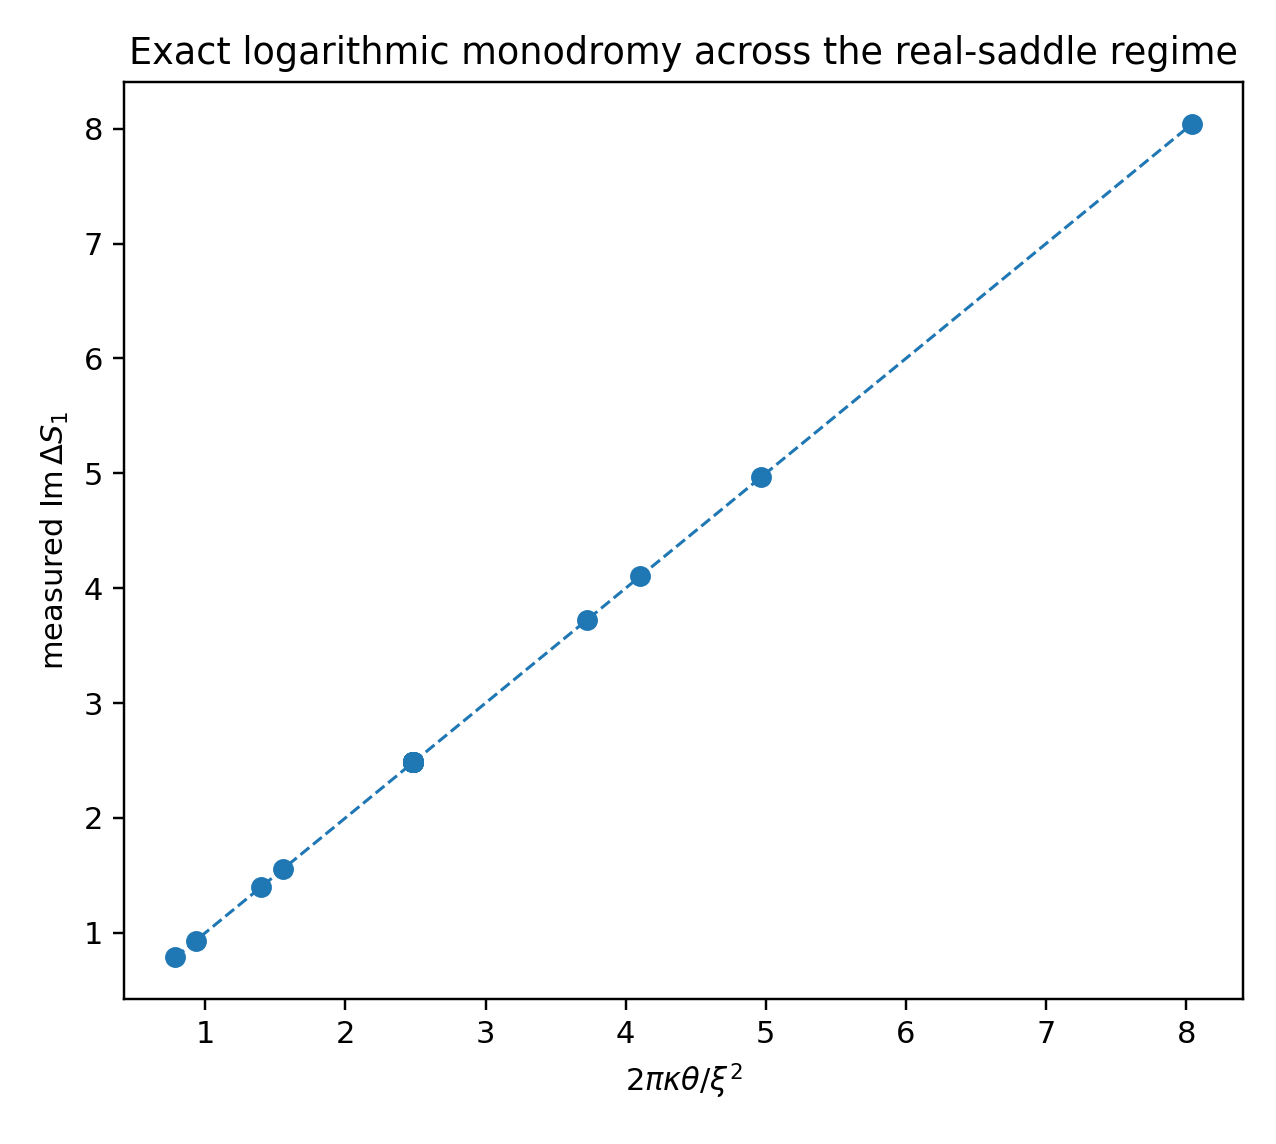
\includegraphics[width=0.72\textwidth]{../figures/heston_generalization_monodromy.png}
\caption{Observed adjacent-sheet imaginary action versus the monodromy prediction $2\pi\kappa\theta/\xi^2$ for all 25 one-parameter sweep points. The points lie on the identity line to numerical precision.}
\label{fig:generalmonodromy}
\end{figure}

The real part $\operatorname{Re}\Delta S_1$ is not universal: it changes smoothly with the endpoint, maturity and Heston coefficients. This is exactly the expected structure. The logarithmic sheet fixes the imaginary increment, whereas the real singulant records the parameter-dependent steepest-descent cost of reaching the adjacent stationary point.

\subsection{Topological stability of the Stokes integer}
At each sweep point we repeat the Picard--Lefschetz flow test using phase offsets $\vartheta_1\pm0.02$. The dual cycle has no Bromwich intersection below the wall and one negatively oriented intersection above it:
\begin{equation}
 \boxed{\langle\Gamma_B,\mathcal K_1\rangle:0\longrightarrow-1}
 \qquad\text{at all 25 points.}
 \label{eq:globaljump}
\end{equation}
The result is displayed in Figure~\ref{fig:generaltopology}.

\begin{figure}[H]
\centering
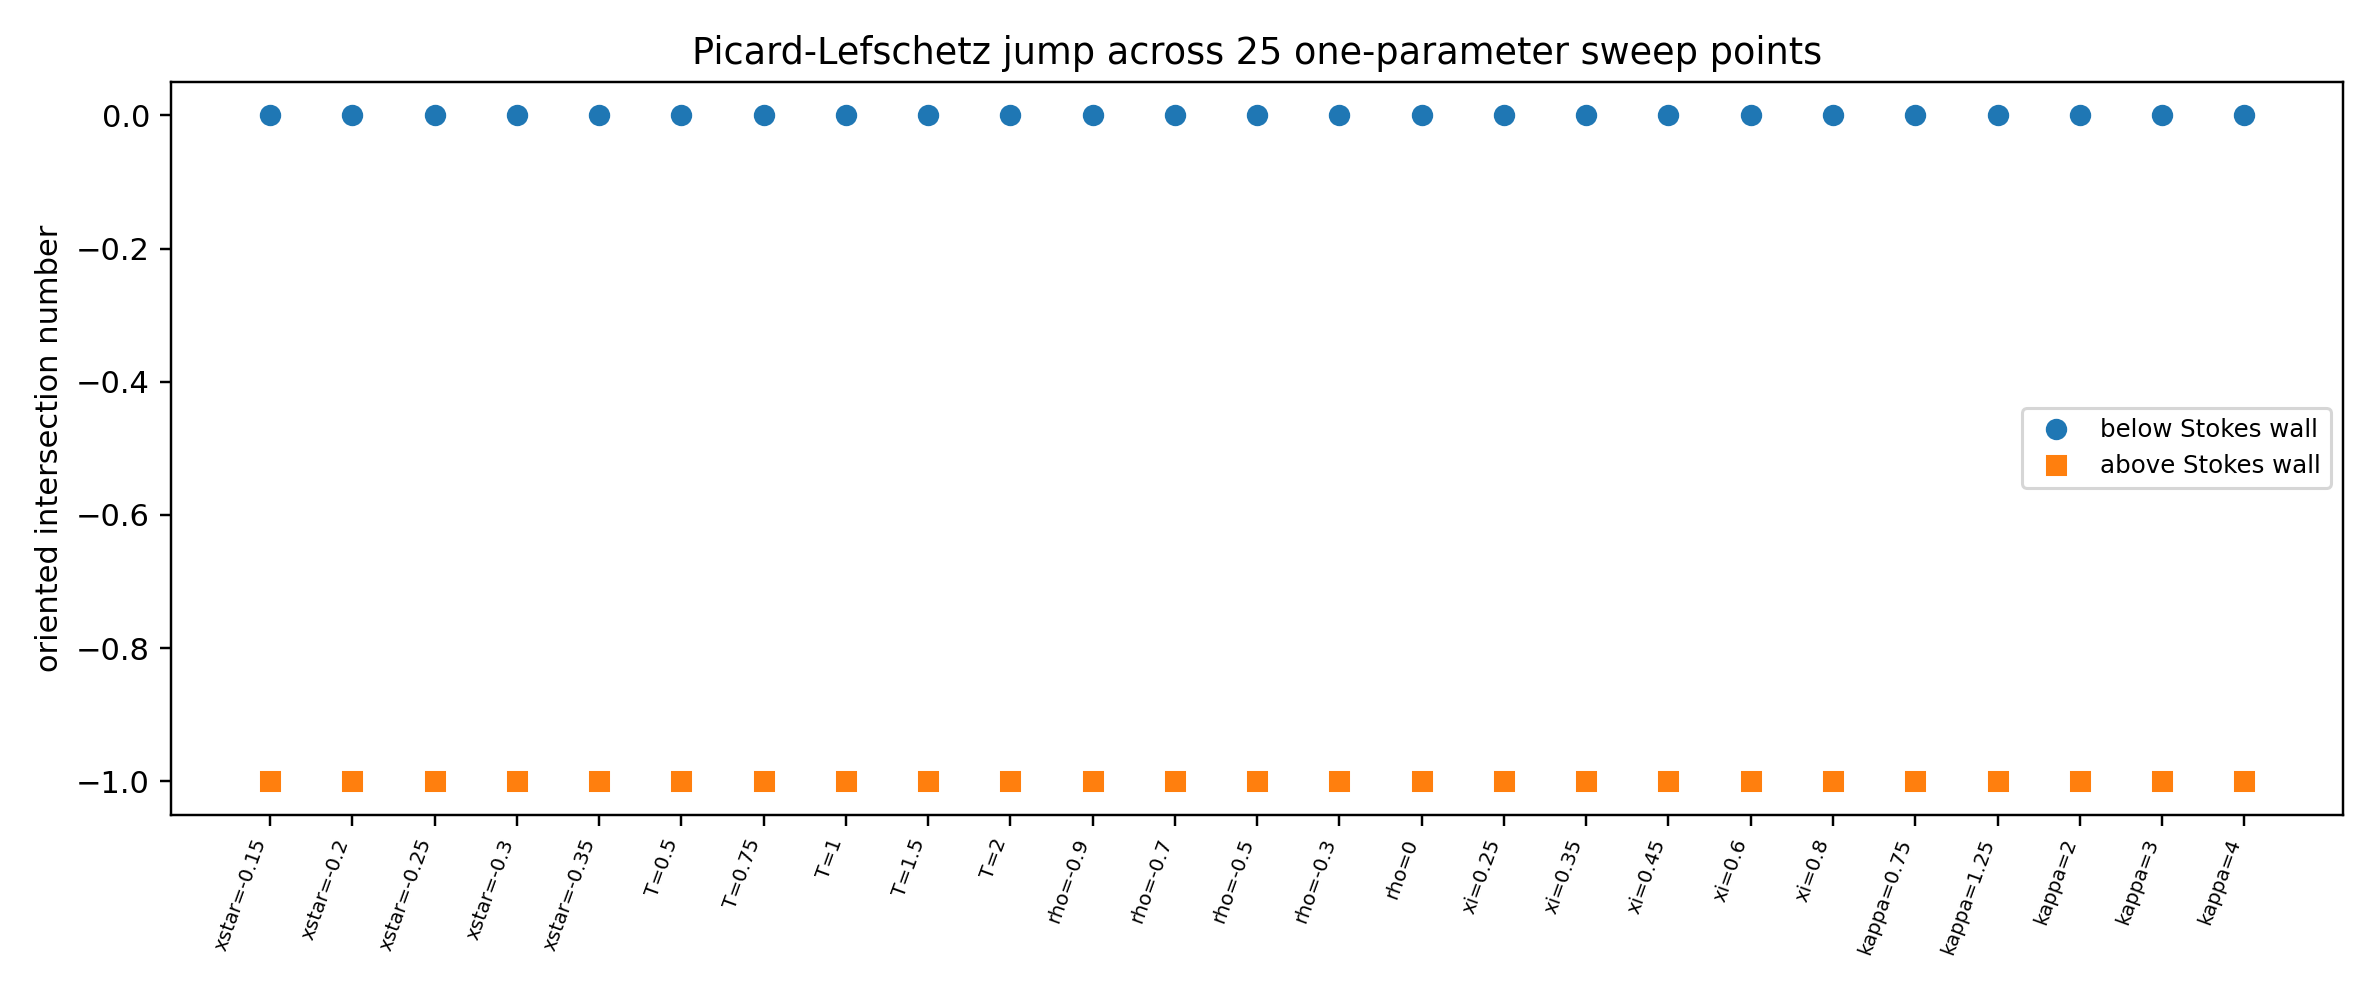
\includegraphics[width=0.96\textwidth]{../figures/heston_generalization_topology.png}
\caption{Oriented Bromwich--dual-cycle intersection numbers immediately below and above the secondary Stokes wall across the complete one-parameter sweep. The jump is identically $0\to-1$.}
\label{fig:generaltopology}
\end{figure}

This stability has a simple topological interpretation. Suppose the adjacent saddle remains nondegenerate, the first two moment singularities remain distinct, and the relevant thimble endpoints do not cross the Bromwich contour or another singular endpoint during a parameter deformation. The intersection number is then an integer homotopy invariant. Hence the benchmark value $S_{01}^{\rm PL}=-1$ persists throughout the connected component. The numerical sweep is consistent with this continuation principle and upgrades the benchmark thimble calculation from an isolated observation to a parameter-domain statement, subject to the stated nondegeneracy assumptions.

\subsection{High-order Borel check at the sweep extremes}
We also test whether the continued adjacent action remains visible from the perturbative sector. To avoid conflating finite-order amplitude extraction with topology, this test uses only the location of the secondary conformal-Borel singularity. Forty physical-saddle coefficients are generated at the two extremes of each of the five parameter axes. The nearest pole of the relevant Pad\'e condensation is then compared with the independently continued $\Delta S_1$.

Across these ten extreme points the median relative location gap is $2.15\%$, while the largest observed gap is $4.30\%$ for $T=2$. Figure~\ref{fig:generalborel} summarizes the result. The precision is lower than the 75-coefficient benchmark, as expected, but every extreme point retains a secondary Pad\'e feature within $5\%$ of the independently calculated adjacent action.

\begin{figure}[H]
\centering
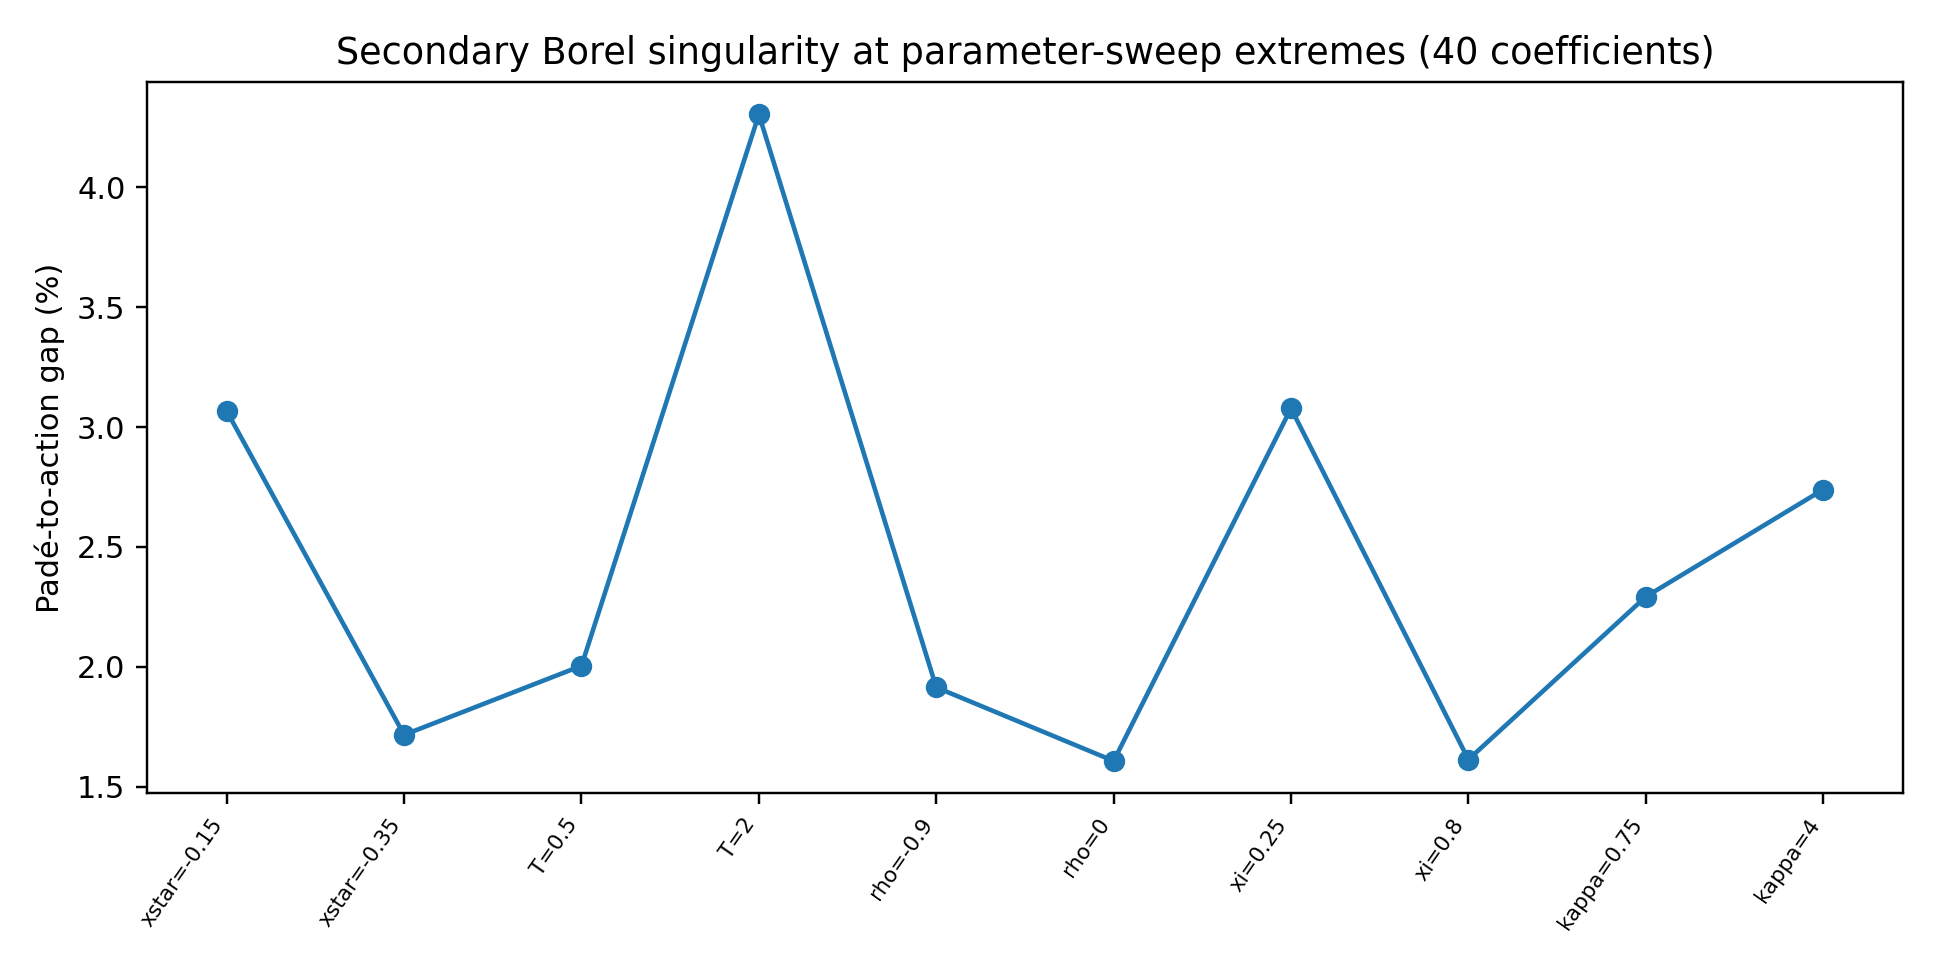
\includegraphics[width=0.88\textwidth]{../figures/heston_generalization_borel_extremes.png}
\caption{Relative distance between the independently continued adjacent action and the corresponding secondary conformal-Borel Pad\'e feature at the two extremes of each parameter axis, using 40 perturbative coefficients.}
\label{fig:generalborel}
\end{figure}

Direct finite-order extraction of the Stokes \emph{amplitude} is less uniform over the sweep. This is not surprising: the residue representation is exponentially sensitive to small pole-location errors and the adjacent fluctuation series itself can lose uniformity near a degenerate saddle. We therefore use the integer Picard--Lefschetz continuation, rather than a fixed-$\varepsilon$ residue estimate, as the robust parameter-domain diagnostic of the Stokes multiplier.

\subsection{A fold caustic and complex-saddle continuation in the correlation direction}
The continuation reveals a genuine boundary just beyond the original interval in $\rho$.  In the relevant adjacent sheet there are two real stationary points for sufficiently negative correlation.  As $\rho$ is increased, these stationary points approach one another.  Their collision is determined by the double-stationary-point conditions
\begin{equation}
 \Phi'(p_c;\rho_c)=0,\qquad
 \Phi''(p_c;\rho_c)=0.
 \label{eq:causticconditions}
\end{equation}
A high-precision simultaneous solve gives
\begin{equation}
 \boxed{\rho_c=0.0299495156775,\qquad p_c=-13.4709103772980.}
 \label{eq:rhocrit}
\end{equation}
The approach of the adjacent Hessian to zero is shown in Figure~\ref{fig:rhocaustic}.

\begin{figure}[H]
\centering
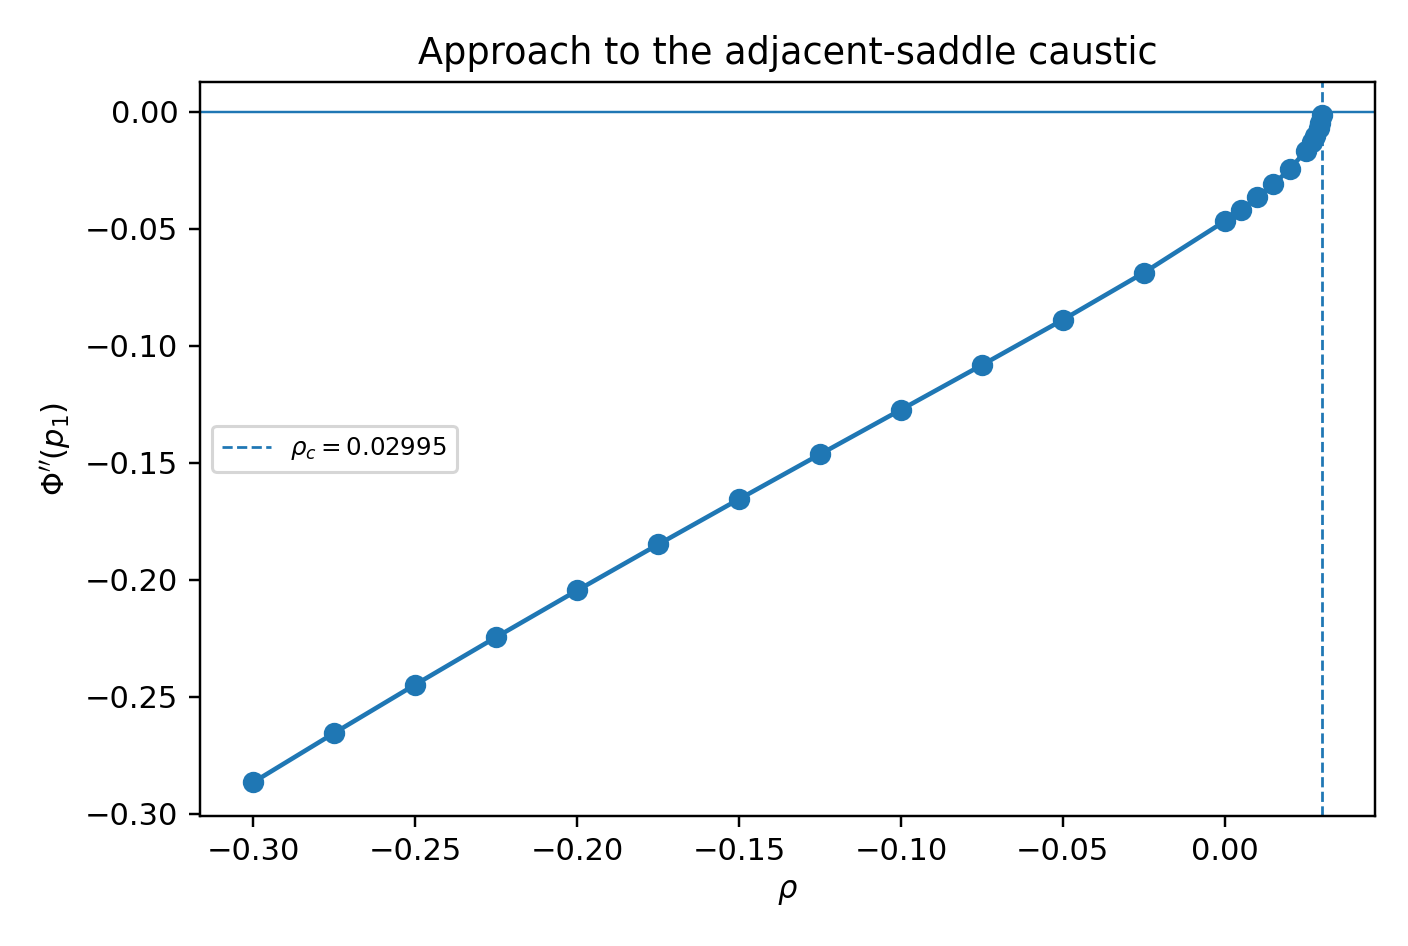
\includegraphics[width=0.72\textwidth]{../figures/heston_generalization_rho_caustic.png}
\caption{Approach to the adjacent-saddle fold in the correlation direction. At $\rho=\rho_c$ the quadratic saddle approximation fails because $\Phi''(p_1)\to0$.}
\label{fig:rhocaustic}
\end{figure}

The collision can be continued through the fold.  Below $\rho_c$ the two relevant stationary points are real; at $\rho_c$ they coalesce; above $\rho_c$ they continue as a complex-conjugate pair.  Figure~\ref{fig:rhofoldreal} shows the real components and Figure~\ref{fig:rhofoldimag} shows the birth of the imaginary components.  For example, already at $\rho=0.05$ the pair is approximately $p\simeq-13.6\pm0.46\,\ii$, and it separates further as $\rho$ increases.

\begin{figure}[H]
\centering
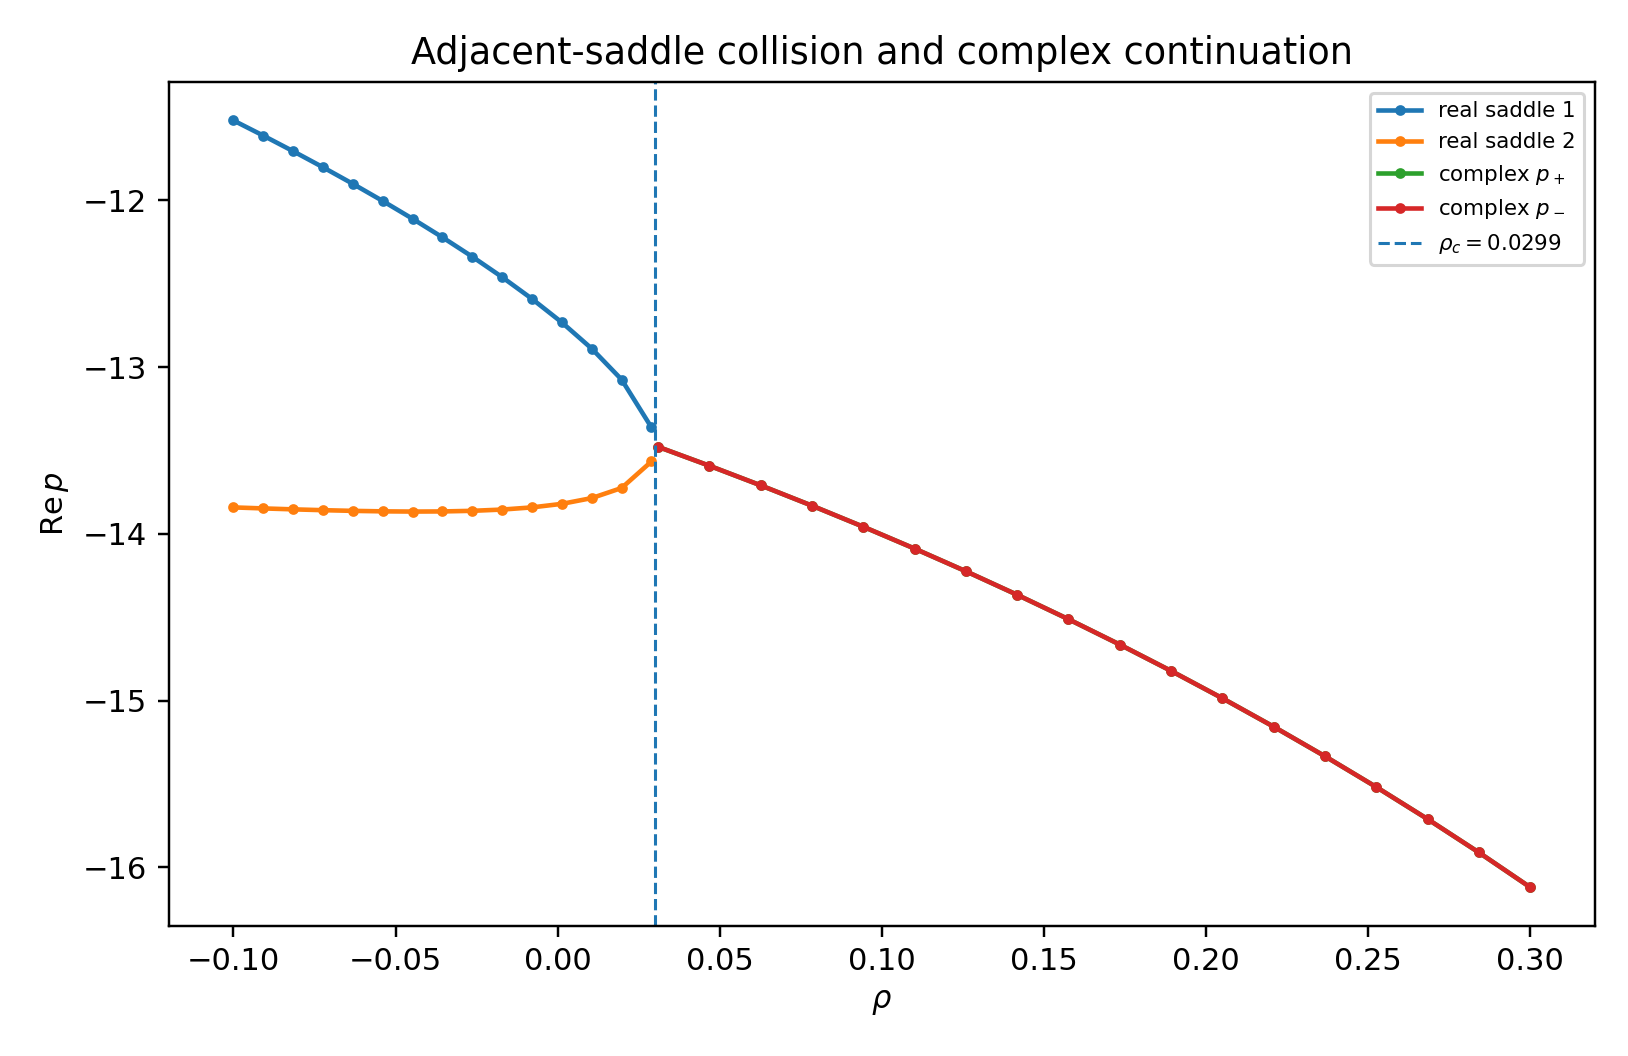
\includegraphics[width=0.78\textwidth]{../figures/heston_rho_saddle_node_real.png}
\caption{Real part of the adjacent stationary points across the correlation fold. Two real saddles coalesce at $\rho_c$ and continue as a complex-conjugate pair.}
\label{fig:rhofoldreal}
\end{figure}

\begin{figure}[H]
\centering
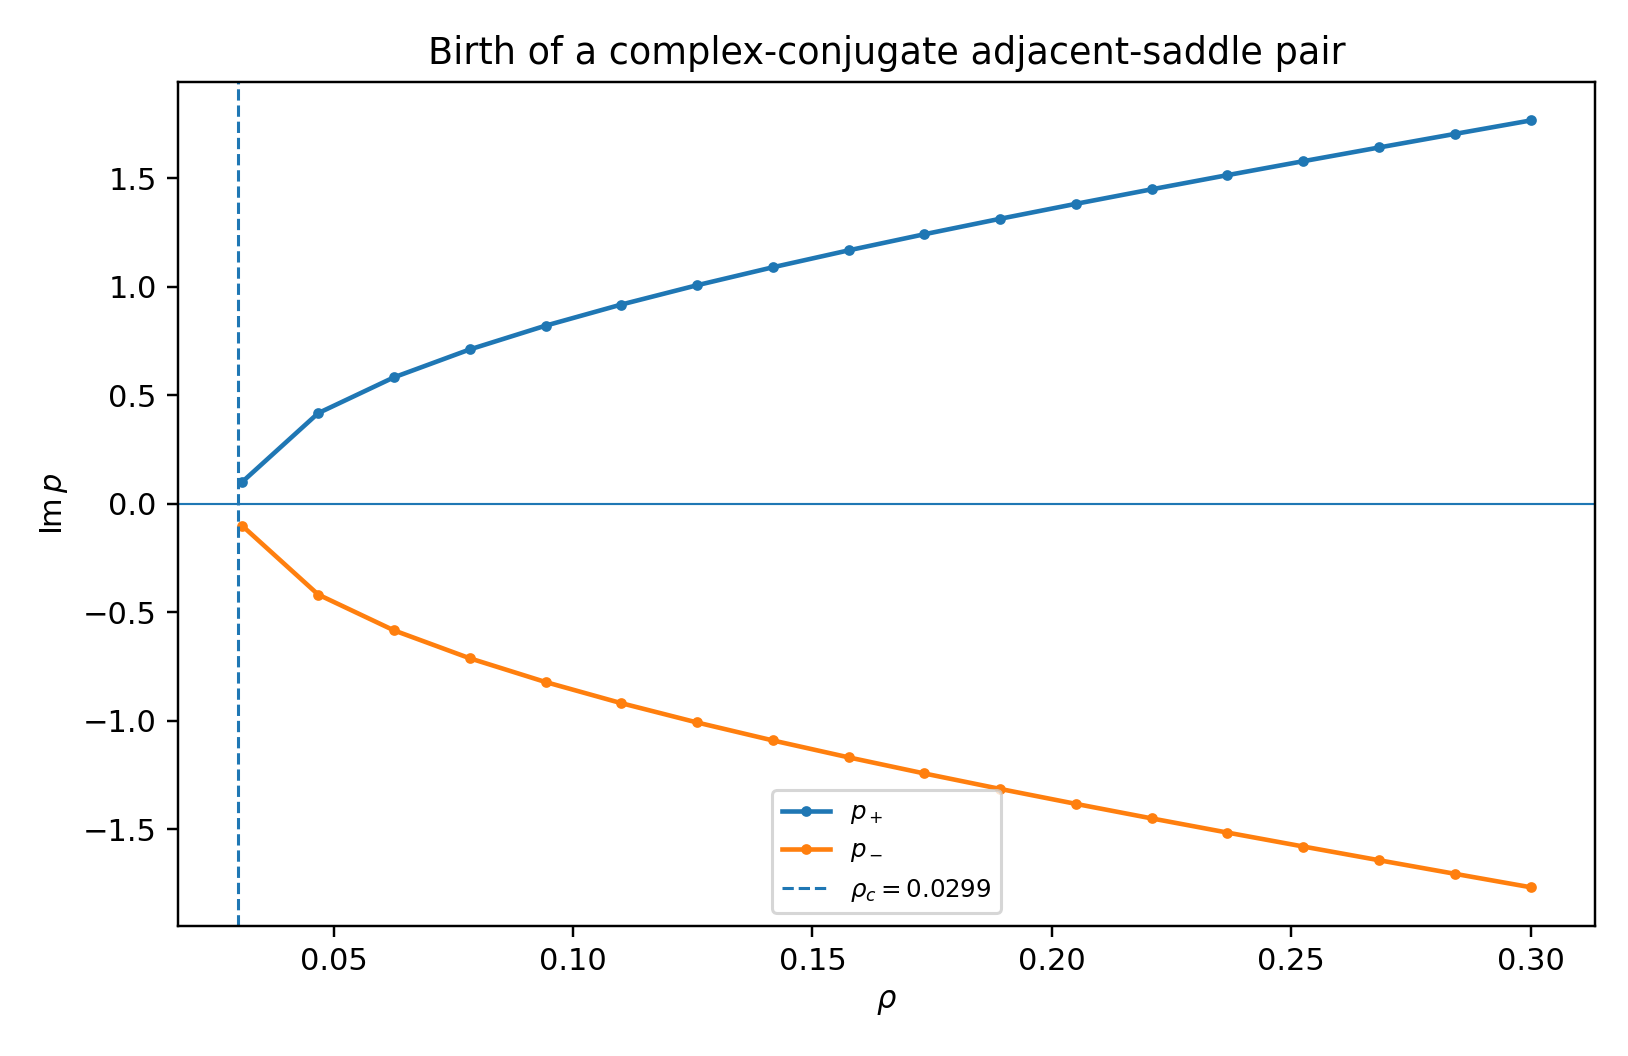
\includegraphics[width=0.78\textwidth]{../figures/heston_rho_saddle_node_imag.png}
\caption{Imaginary parts of the continued adjacent stationary points. The imaginary component is zero below the fold and becomes nonzero for the complex-conjugate pair above $\rho_c$.}
\label{fig:rhofoldimag}
\end{figure}

The ordinary Gaussian saddle expansion assumes a nonzero quadratic Hessian. Accordingly its coefficients become badly conditioned as $\rho\to\rho_c^-$. For example, at $\rho=0$ the adjacent series already begins with $1+19.53\,\varepsilon+2.58\times10^3\varepsilon^2+\cdots$. This is not evidence against resurgence. It is the standard signal that stationary points are approaching a fold, where a cubic normal form and an Airy-type uniform approximation replace two separate Gaussian saddle expansions \citep{chester1957}. The correct continuation across $\rho_c$ should therefore be formulated as a uniform resurgent treatment of the coalescing pair.

\subsection{Anti-Stokes boundaries and exchange of exponential dominance}
A second type of boundary appears even when the adjacent stationary point remains nondegenerate.  The relative exponential weight of the adjacent sector is
\begin{equation}
 \exp\!\left[-\frac{\Delta S_1}{\varepsilon}\right].
\end{equation}
For positive real $\varepsilon$, the two sectors have equal exponential magnitude when
\begin{equation}
 \boxed{\operatorname{Re}\Delta S_1=0.}
 \label{eq:antistokescondition}
\end{equation}
This is an anti-Stokes condition: it concerns equality of magnitudes, in contrast with the Stokes condition, which aligns phases and controls the thimble jump.

Along the maturity slice with all other parameters fixed at the benchmark values, the real singulant decreases continuously from $6.12676$ at $T=0.5$ to $0.17150$ at $T=2.5$, and then changes sign.  Solving Eq.~\eqref{eq:antistokescondition} gives
\begin{equation}
 \boxed{T_A=2.678155844206.}
 \label{eq:Tantistokes}
\end{equation}
The continuation is shown in Figure~\ref{fig:Tantistokes}.  For $T<T_A$ the adjacent sector is exponentially subdominant relative to the physical saddle; at $T=T_A$ the two sectors have equal exponential magnitude; for $T>T_A$ the hierarchy based on the physical sector must be reorganised.

\begin{figure}[H]
\centering
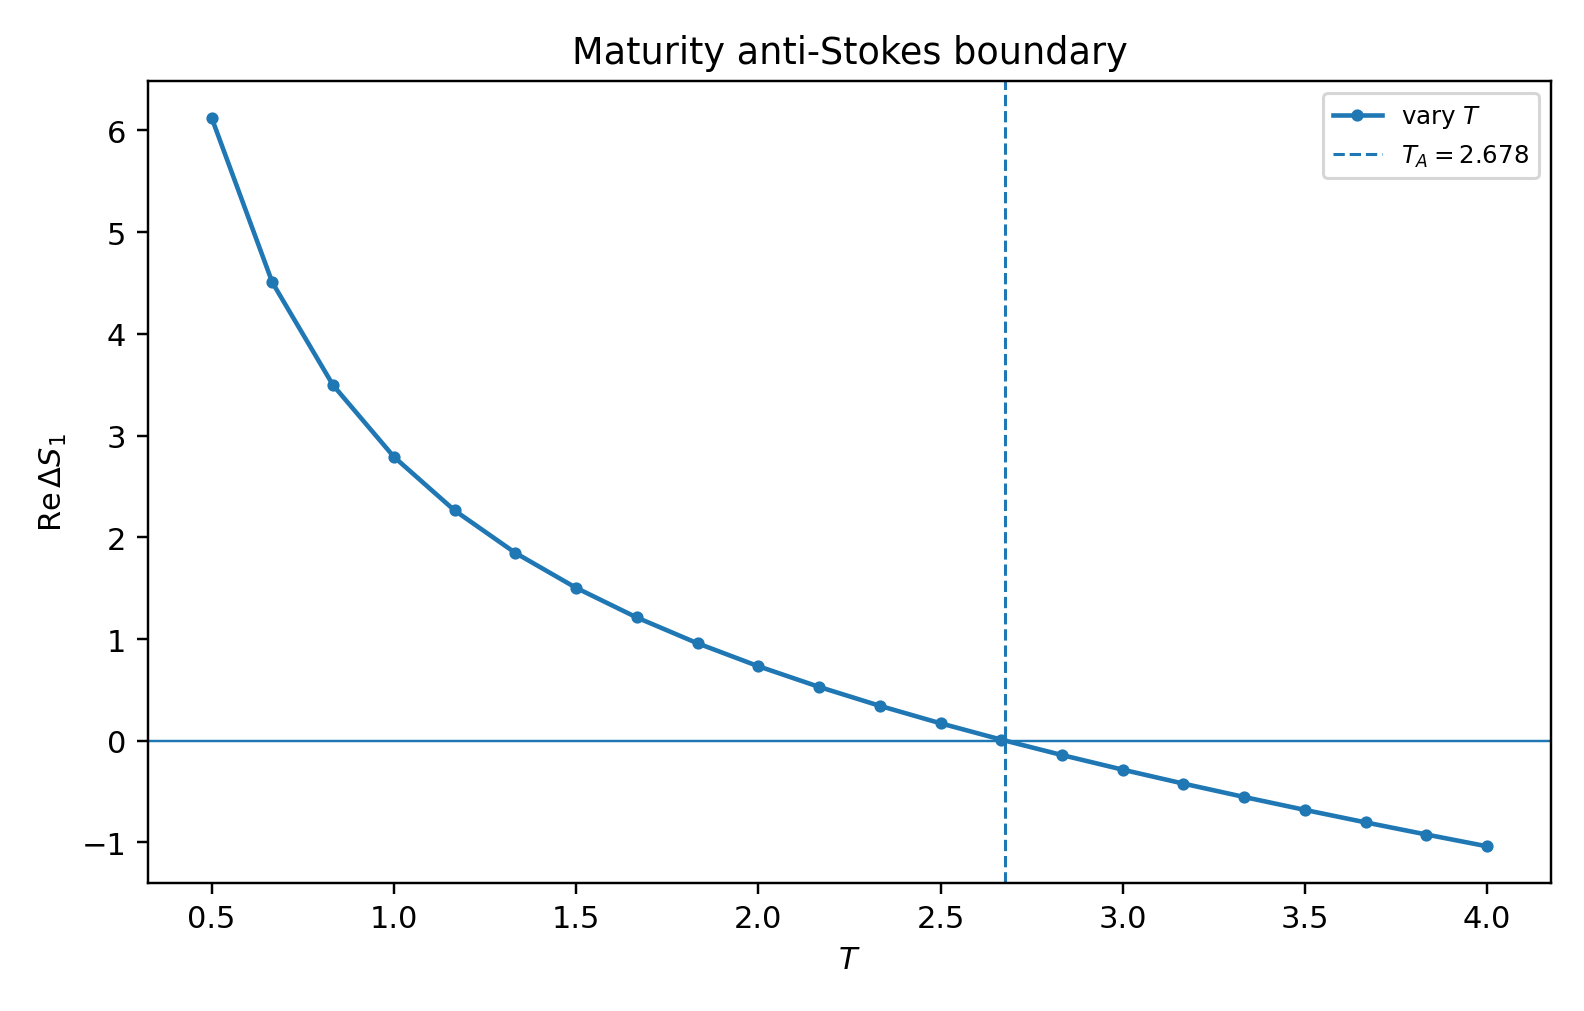
\includegraphics[width=0.78\textwidth]{../figures/heston_phase_boundary_T.png}
\caption{Maturity continuation of the adjacent singulant. The anti-Stokes point $T_A$ occurs where $\operatorname{Re}\Delta S_1$ crosses zero while the monodromy-fixed imaginary part remains nonzero.}
\label{fig:Tantistokes}
\end{figure}

An analogous dominance exchange occurs along the mean-reversion slice.  Solving
\begin{equation}
 \operatorname{Re}\Delta S_1(\kappa_A)=0
\end{equation}
with the remaining benchmark parameters fixed gives
\begin{equation}
 \boxed{\kappa_A=5.470788617678.}
 \label{eq:kappaantistokes}
\end{equation}
Figure~\ref{fig:kappaantistokes} displays this crossing.  In this direction the imaginary singulant is not constant; it follows the exact monodromy law $2\pi\kappa\theta/\xi^2$ while the real part passes through zero.

\begin{figure}[H]
\centering
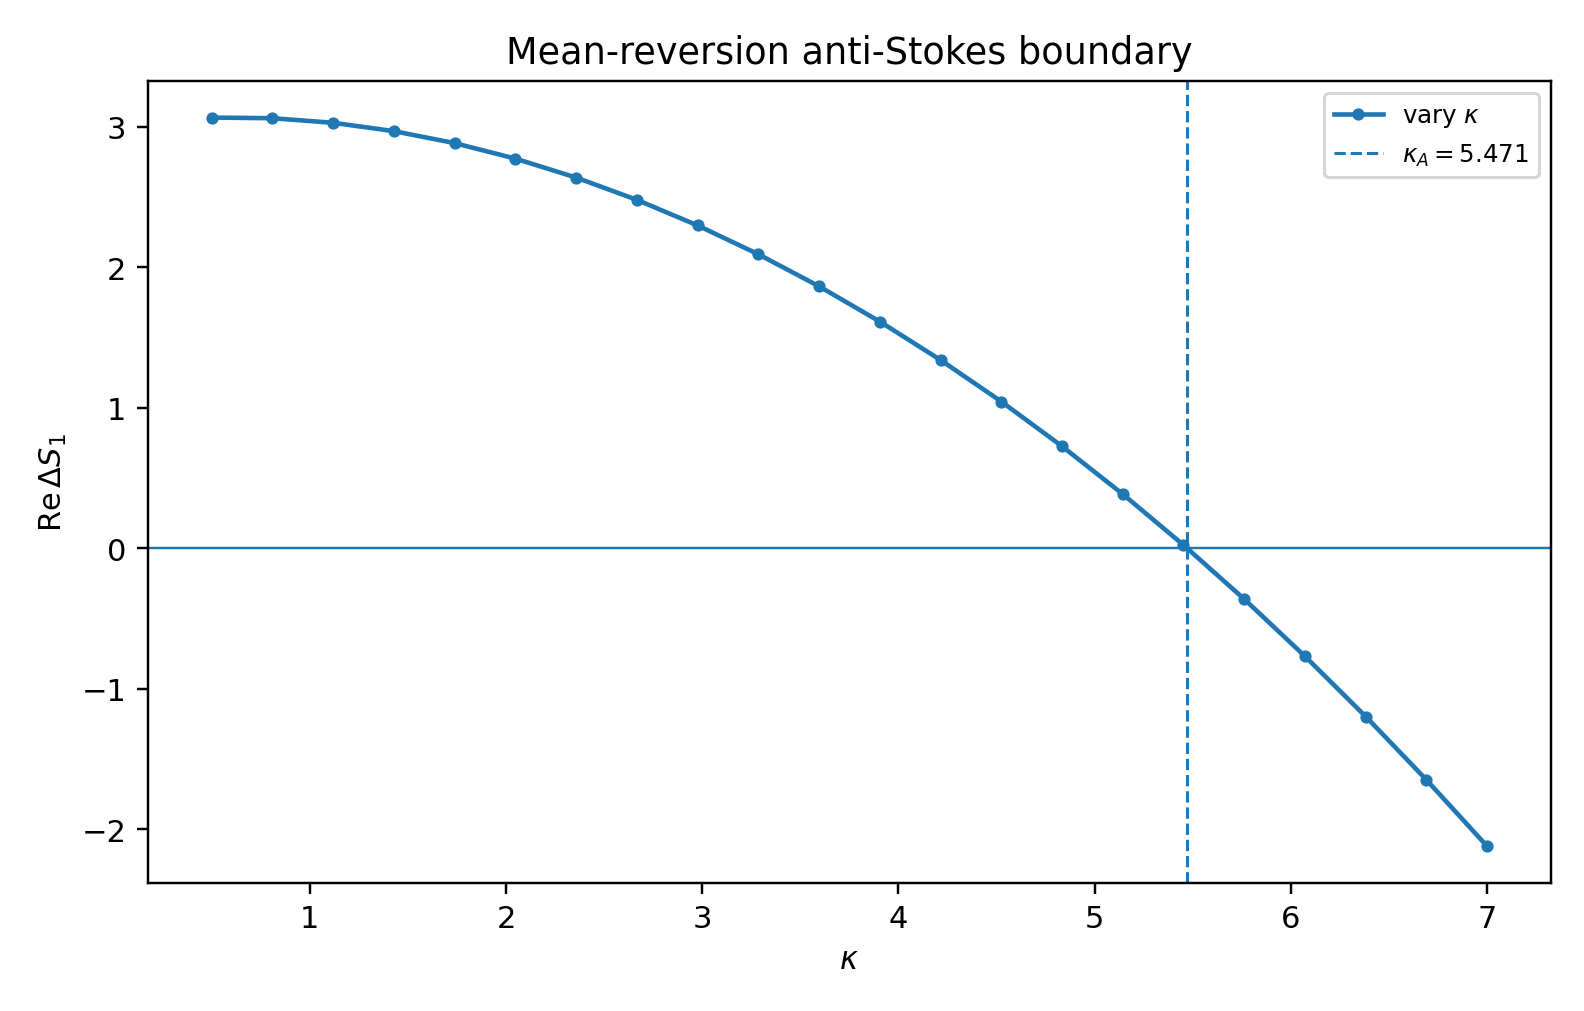
\includegraphics[width=0.78\textwidth]{../figures/heston_phase_boundary_kappa.png}
\caption{Mean-reversion continuation of the adjacent singulant. The anti-Stokes point $\kappa_A$ is the zero of $\operatorname{Re}\Delta S_1$ along the benchmark slice.}
\label{fig:kappaantistokes}
\end{figure}

\subsection{A first resurgent phase diagram}
The combined continuation therefore produces a phase structure rather than a globally identical two-sector expansion.  Three pieces of the geometry are robust on the tested connected nondegenerate region: the logarithmic monodromy, the smooth continuation of the secondary Borel location, and the Picard--Lefschetz jump $0\to-1$.  Two different codimension-one boundaries then organise the breakdown of this local description:
\begin{enumerate}
 \item a \emph{fold/caustic surface}, defined by $\Phi'=\Phi''=0$, where separate Gaussian saddle expansions cease to be uniform and real saddles may continue as a complex-conjugate pair;
 \item an \emph{anti-Stokes surface}, defined by $\operatorname{Re}\Delta S_1=0$, where the relative exponential hierarchy of the two sectors changes.
\end{enumerate}
On the benchmark one-dimensional slices the first observed representatives are summarised in Table~\ref{tab:phaseboundaries}.

\begin{table}[H]
\centering
\begin{tabular}{lll}
\toprule
Boundary & Condition & Benchmark-slice location \\
\midrule
Correlation fold & $\Phi'=\Phi''=0$ & $\rho_c=0.0299495156775$ \\
Maturity anti-Stokes & $\operatorname{Re}\Delta S_1=0$ & $T_A=2.678155844206$ \\
Mean-reversion anti-Stokes & $\operatorname{Re}\Delta S_1=0$ & $\kappa_A=5.470788617678$ \\
\bottomrule
\end{tabular}
\caption{First numerically resolved boundaries of the resurgent phase structure along benchmark parameter slices. These are slice intersections of higher-dimensional boundary surfaces, not universal constants of the Heston model.}
\label{tab:phaseboundaries}
\end{table}

These observations suggest a sharper continuation principle.  On a connected parameter domain where the relevant saddles are simple, the moment singularities remain ordered and no thimble endpoint changes homology, the connection integer remains topologically fixed while $\Delta S_1$ deforms smoothly.  Caustics require a uniform local transseries, and anti-Stokes surfaces require a change of dominant exponential basis.  A global resurgent description of the Heston family should therefore be organised as a parameter-space atlas of such local transseries rather than as one expansion valid everywhere.


\section{Uniform Airy resolution of the correlation fold}
The correlation caustic is a genuine breakdown of the isolated Gaussian saddle expansion because the quadratic Hessian vanishes.  Let
\begin{equation}
 q=p-p_c,\qquad \delta\rho=\rho-\rho_c.
\end{equation}
At the fold, $\Phi_p=\Phi_{pp}=0$, and the local phase has the cubic normal form
\begin{equation}
 \Phi(p,\rho)=\Phi_c+\Phi_\rho\,\delta\rho
 +\Phi_{p\rho}\,\delta\rho\,q
 +\frac{\Phi_{ppp}}{6}q^3+\cdots.
 \label{eq:foldnormal}
\end{equation}
For the benchmark slice we obtain
\begin{equation}
 \Phi_{p\rho}=-0.355264810623,\qquad
 \Phi_{ppp}=-0.068628748380.
\end{equation}
The stationarity condition derived from Eq.~\eqref{eq:foldnormal} gives
\begin{equation}
 q^2=\alpha\,\delta\rho,\qquad
 \alpha=-\frac{2\Phi_{p\rho}}{\Phi_{ppp}}=-10.3532358964.
 \label{eq:foldsqrt}
\end{equation}
Hence the two real saddles for $\delta\rho<0$ split as
\begin{equation}
 |p_+-p_-|\sim 2C_\rho(\rho_c-\rho)^{1/2},\qquad
 C_\rho=3.21764446395,
\end{equation}
while their action difference obeys the characteristic fold law
\begin{equation}
 |\Phi(p_+)-\Phi(p_-)|\sim
 C_S(\rho_c-\rho)^{3/2},\qquad
 C_S=1.52415446818.
 \label{eq:foldaction}
\end{equation}
Direct high-precision Heston roots reproduce both the $1/2$ and $3/2$ exponents over several decades; the comparisons are shown in Figures~\ref{fig:airysaddles} and \ref{fig:airyaction}.

\begin{figure}[H]
\centering
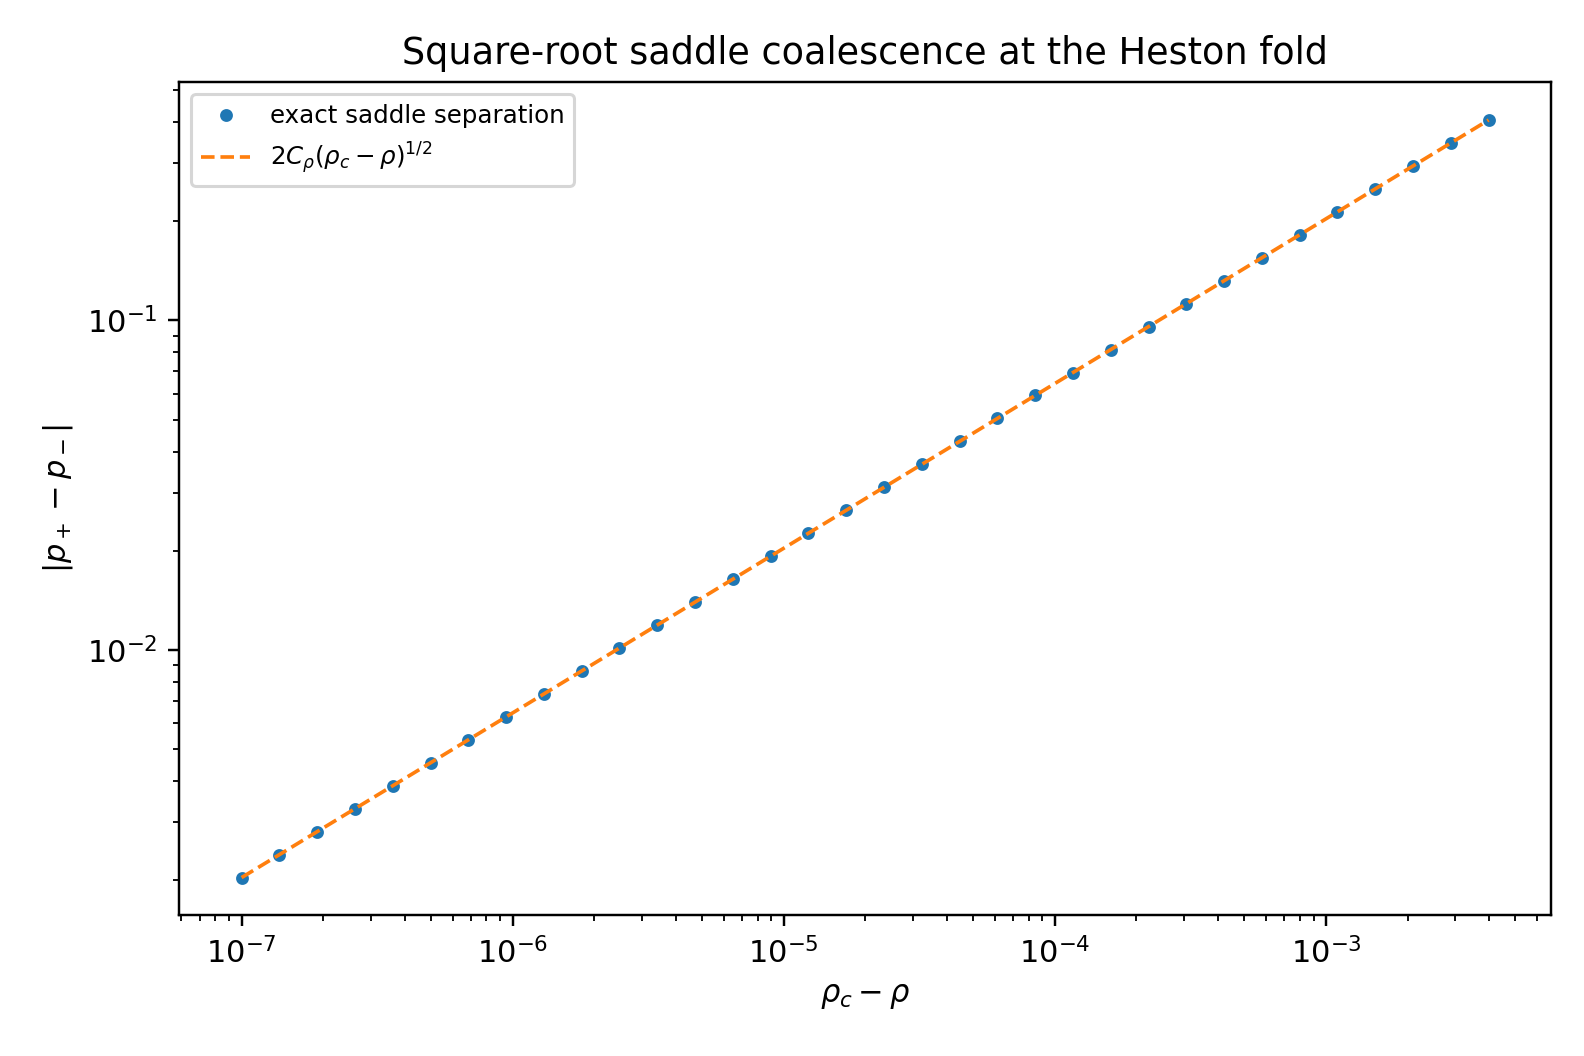
\includegraphics[width=0.76\textwidth]{../figures/heston_airy_saddle_scaling.png}
\caption{Exact separation of the coalescing Heston stationary points compared with the square-root fold law from the cubic normal form.}
\label{fig:airysaddles}
\end{figure}

\begin{figure}[H]
\centering
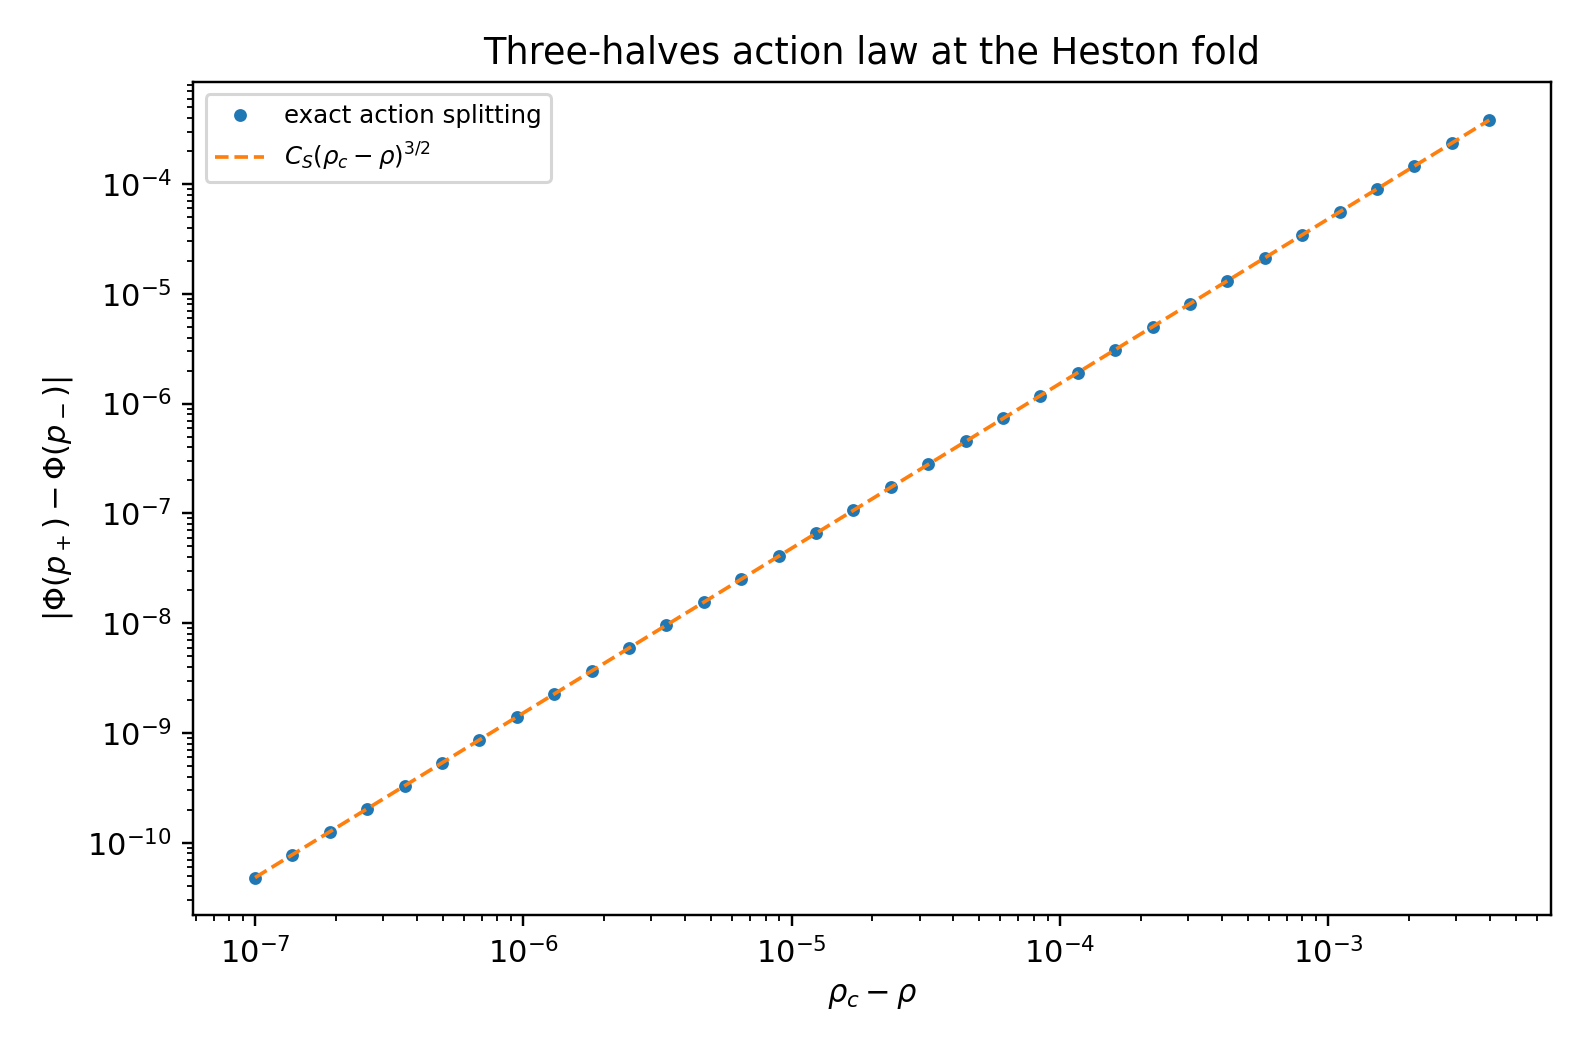
\includegraphics[width=0.76\textwidth]{../figures/heston_airy_action_scaling.png}
\caption{Exact action splitting of the coalescing pair compared with the $(\rho_c-\rho)^{3/2}$ fold prediction.}
\label{fig:airyaction}
\end{figure}

To obtain a uniform approximation, write $A=\Phi_{ppp}/2$ and rescale $u=A^{1/3}q$.  Equation~\eqref{eq:foldnormal} becomes
\begin{equation}
 \Phi=\Phi_c+\Phi_\rho\delta\rho+\frac{u^3}{3}-\zeta u+\cdots,
\end{equation}
with
\begin{equation}
 \boxed{\zeta=-\frac{\Phi_{p\rho}}{A^{1/3}}\delta\rho
 =-1.09326849050(\rho-\rho_c).}
 \label{eq:airyzeta}
\end{equation}
The fold boundary layer is therefore
\begin{equation}
 Z=\frac{\zeta}{\varepsilon^{2/3}}=O(1),
 \qquad |\rho-\rho_c|=O(\varepsilon^{2/3}).
 \label{eq:airylayer}
\end{equation}
For an analytic transformed amplitude, the Chester--Friedman--Ursell reduction gives the local uniform sector
\begin{equation}
 F_{\rm fold}(\varepsilon,\rho)
 \sim e^{(\Phi_c+\Phi_\rho\delta\rho)/\varepsilon}
 \left[A_0\varepsilon^{1/3}\operatorname{Ai}(Z)
 -B_0\varepsilon^{2/3}\operatorname{Ai}'(Z)+\cdots\right].
 \label{eq:airyuniform}
\end{equation}
The coefficients $A_0,B_0,\ldots$ depend on the transformed Bromwich amplitude and contour orientation, while the scaling variable and catastrophe exponents are fixed by Eq.~\eqref{eq:foldnormal}.  Crucially, $\operatorname{Ai}(0)$ is finite whereas the isolated one-saddle approximation behaves as $Z^{-1/4}$ and diverges at the caustic.  Figures~\ref{fig:airylayer} and \ref{fig:airygaussian} display the universal crossover.  Thus the caustic does not destroy the resurgent description; it changes the correct local basis from separate saddle sectors to a single Airy-uniform sector whose own asymptotic expansions reproduce the appropriate saddle contributions away from the fold.

\begin{figure}[H]
\centering
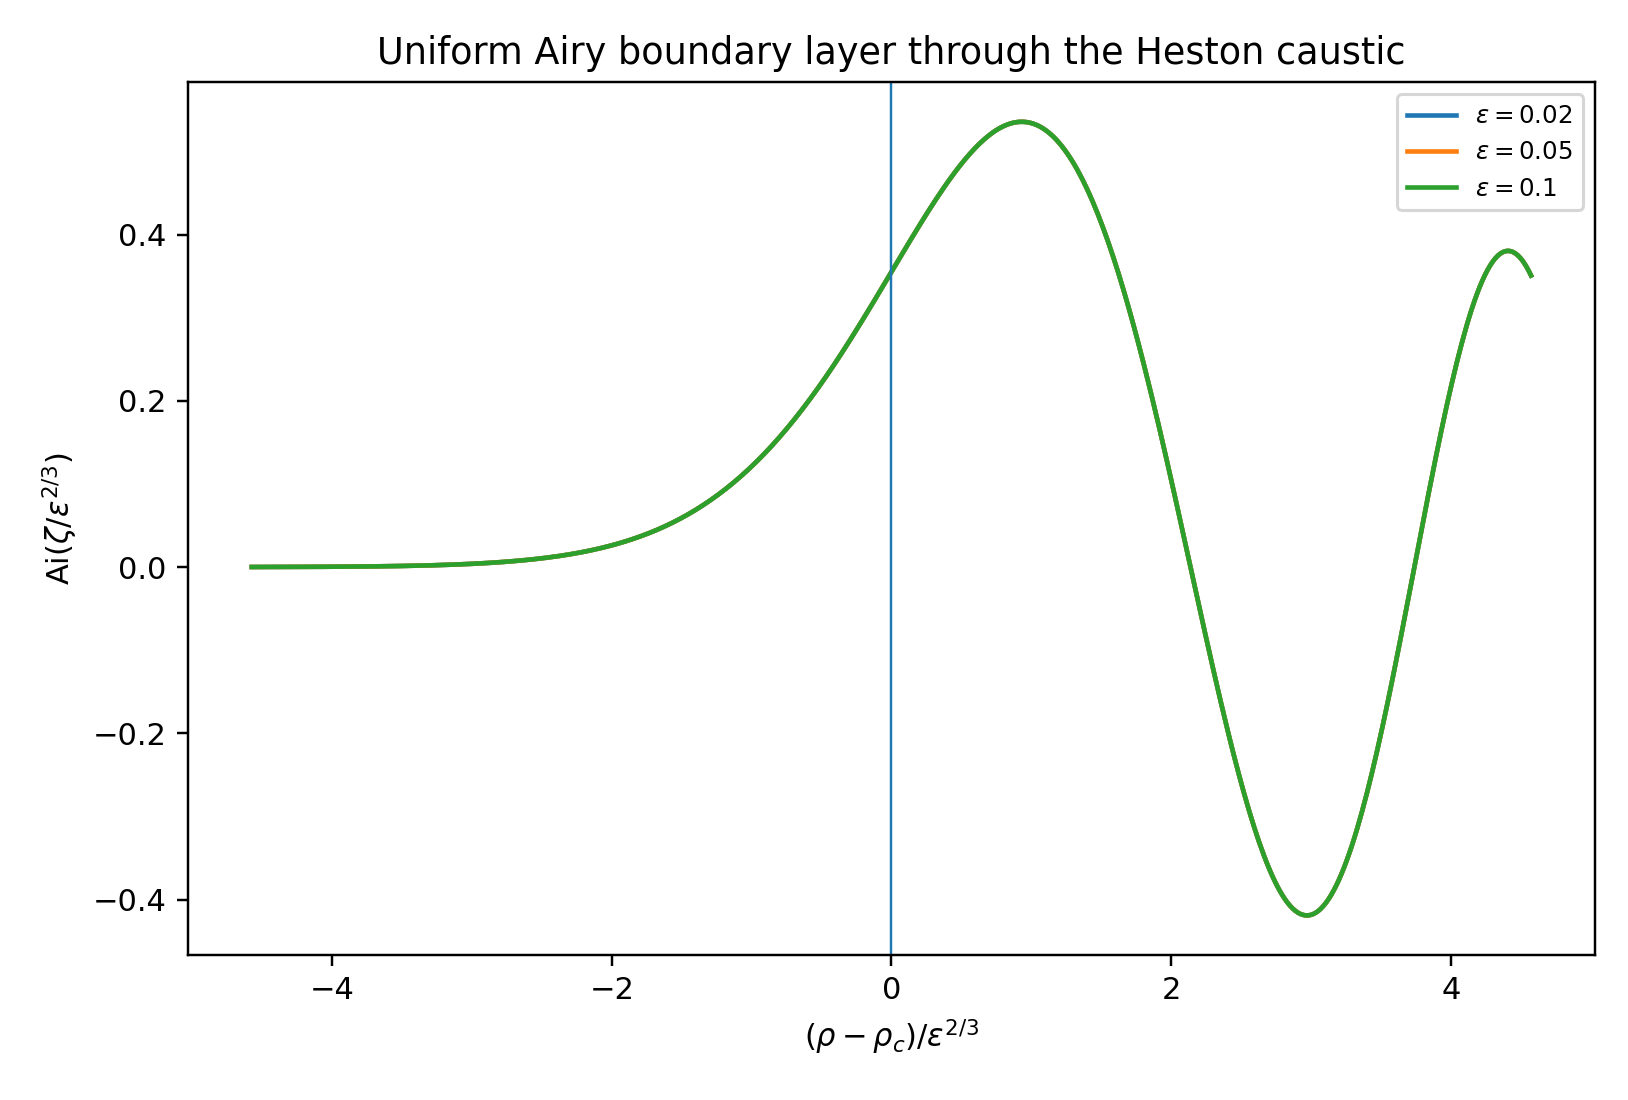
\includegraphics[width=0.76\textwidth]{../figures/heston_uniform_airy_boundary_layer.png}
\caption{Universal Airy boundary layer after scaling $\rho-\rho_c$ by $\varepsilon^{2/3}$. Curves for different noise strengths collapse onto the same canonical profile.}
\label{fig:airylayer}
\end{figure}

\begin{figure}[H]
\centering
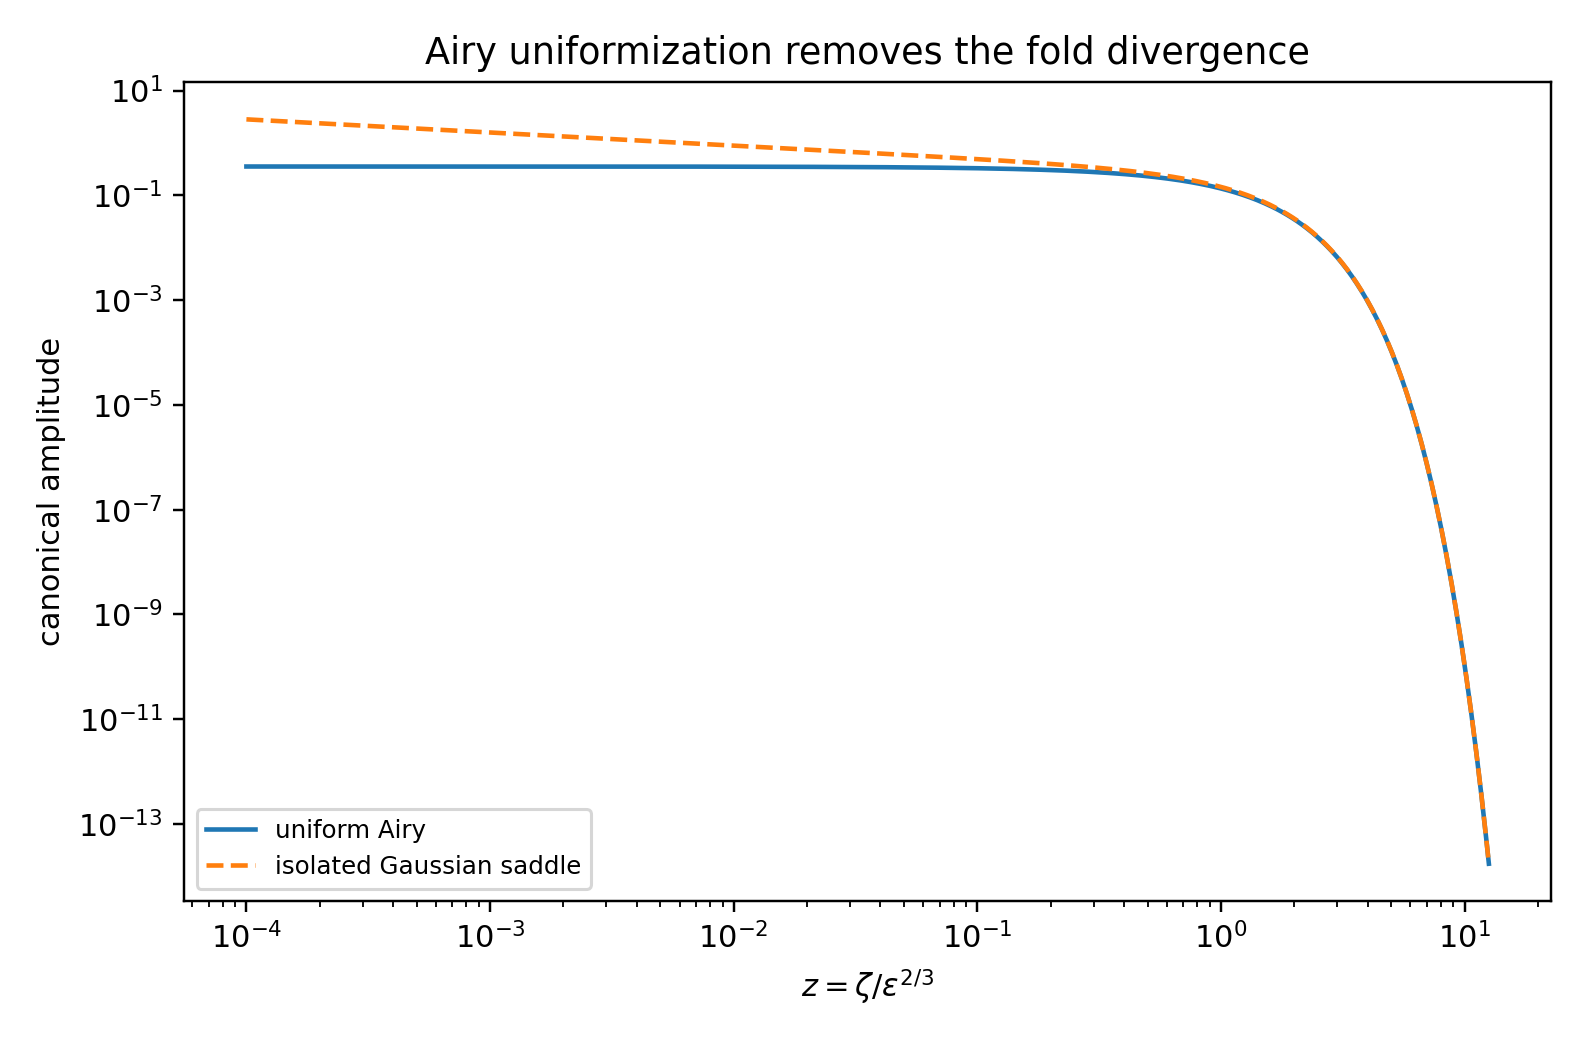
\includegraphics[width=0.76\textwidth]{../figures/heston_uniform_airy_vs_gaussian.png}
\caption{The Airy uniform approximation remains finite at the fold, while the isolated Gaussian-saddle asymptotic diverges as the Hessian vanishes.}
\label{fig:airygaussian}
\end{figure}

\section{Two-dimensional \texorpdfstring{$(T,\rho)$}{(T,rho)} resurgent atlas}
The one-dimensional continuations do not by themselves reveal how the boundaries connect.  We therefore construct a two-dimensional atlas at fixed $x_\star=-0.25$, $\kappa=2$, $\theta=v_0=0.04$ and $\xi=0.45$.  At each real parameter point the adjacent sector is defined invariantly as the \emph{first stationary point between the first two negative moment poles}.  This definition is important: naive Newton continuation can silently jump between stationary points when moment-pole geometry rearranges.

For each $(T,\rho)$ inside the real-adjacent domain we calculate the physical saddle $p_\star$, the first two moment poles, the first adjacent stationary point $p_1$, and
\begin{equation}
 \Delta S_1=\Phi(p_\star)-\Phi(p_1).
\end{equation}
The atlas contains 763 independently resolved parameter points.  Its imaginary part again satisfies
\begin{equation}
 \operatorname{Im}\Delta S_1=2\pi\frac{\kappa\theta}{\xi^2}=2.482246047281
\end{equation}
with maximum relative discrepancy $1.8\times10^{-16}$ on the grid.  Therefore the two-dimensional structure is controlled primarily by the moving real part of the singulant.

Figure~\ref{fig:2dphase} displays $\operatorname{Re}\Delta S_1$.  The solid curve is the caustic $\Phi_p=\Phi_{pp}=0$; the dashed curve is the anti-Stokes locus $\operatorname{Re}\Delta S_1=0$.  The coarse two-dimensional curve crosses the benchmark line $\rho=-0.7$ at
\begin{equation}
 T_A^{(2D)}\approx2.67749,
\end{equation}
consistent to $6.7\times10^{-4}$ with the independently refined one-dimensional value in Eq.~\eqref{eq:Tantistokes}.  This agreement is a useful cross-check that the atlas is tracking the same adjacent sector.

\begin{figure}[H]
\centering
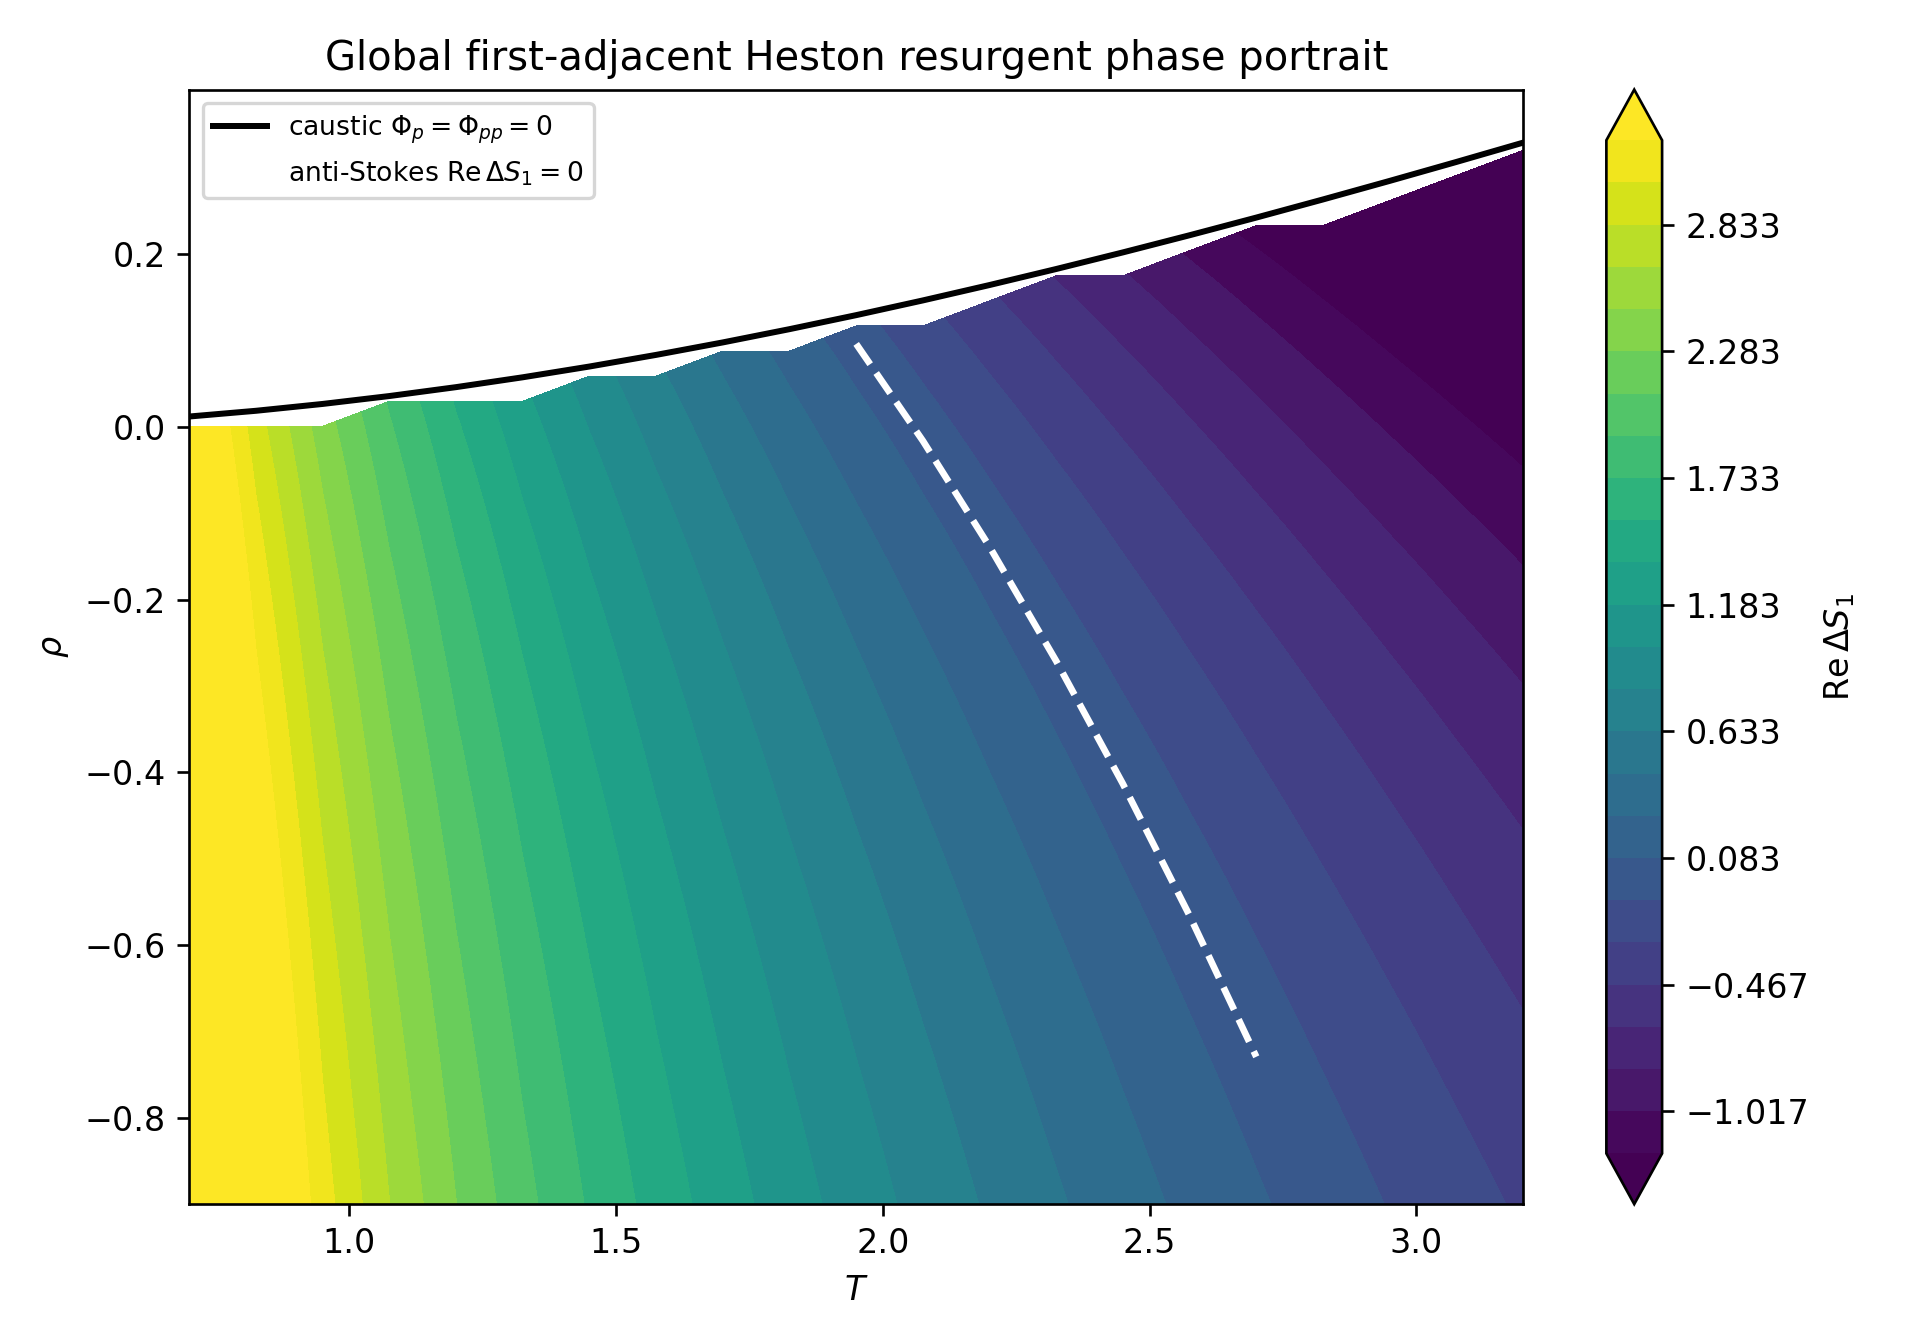
\includegraphics[width=0.86\textwidth]{../figures/heston_T_rho_resurgent_phase_portrait.png}
\caption{Two-dimensional resurgent phase portrait in the $(T,\rho)$ plane. Color gives $\operatorname{Re}\Delta S_1$; the black curve is the fold/caustic and the white dashed curve is the anti-Stokes locus.}
\label{fig:2dphase}
\end{figure}

The Stokes condition concerns phase rather than magnitude.  In the present real-adjacent domain the monodromy keeps $\operatorname{Im}\Delta S_1>0$, so no positive-real-$\varepsilon$ Stokes curve occurs inside the plotted domain.  Instead each parameter point has a Stokes ray in the complex $\varepsilon$ plane at
\begin{equation}
 \vartheta_S(T,\rho)=\arg\Delta S_1(T,\rho).
\end{equation}
Figure~\ref{fig:2dstokes} maps this Stokes-angle field.  On the anti-Stokes curve $\operatorname{Re}\Delta S_1=0$, hence $\vartheta_S=\pi/2$; approaching the caustic changes the appropriate local basis to the Airy sector derived above.

\begin{figure}[H]
\centering
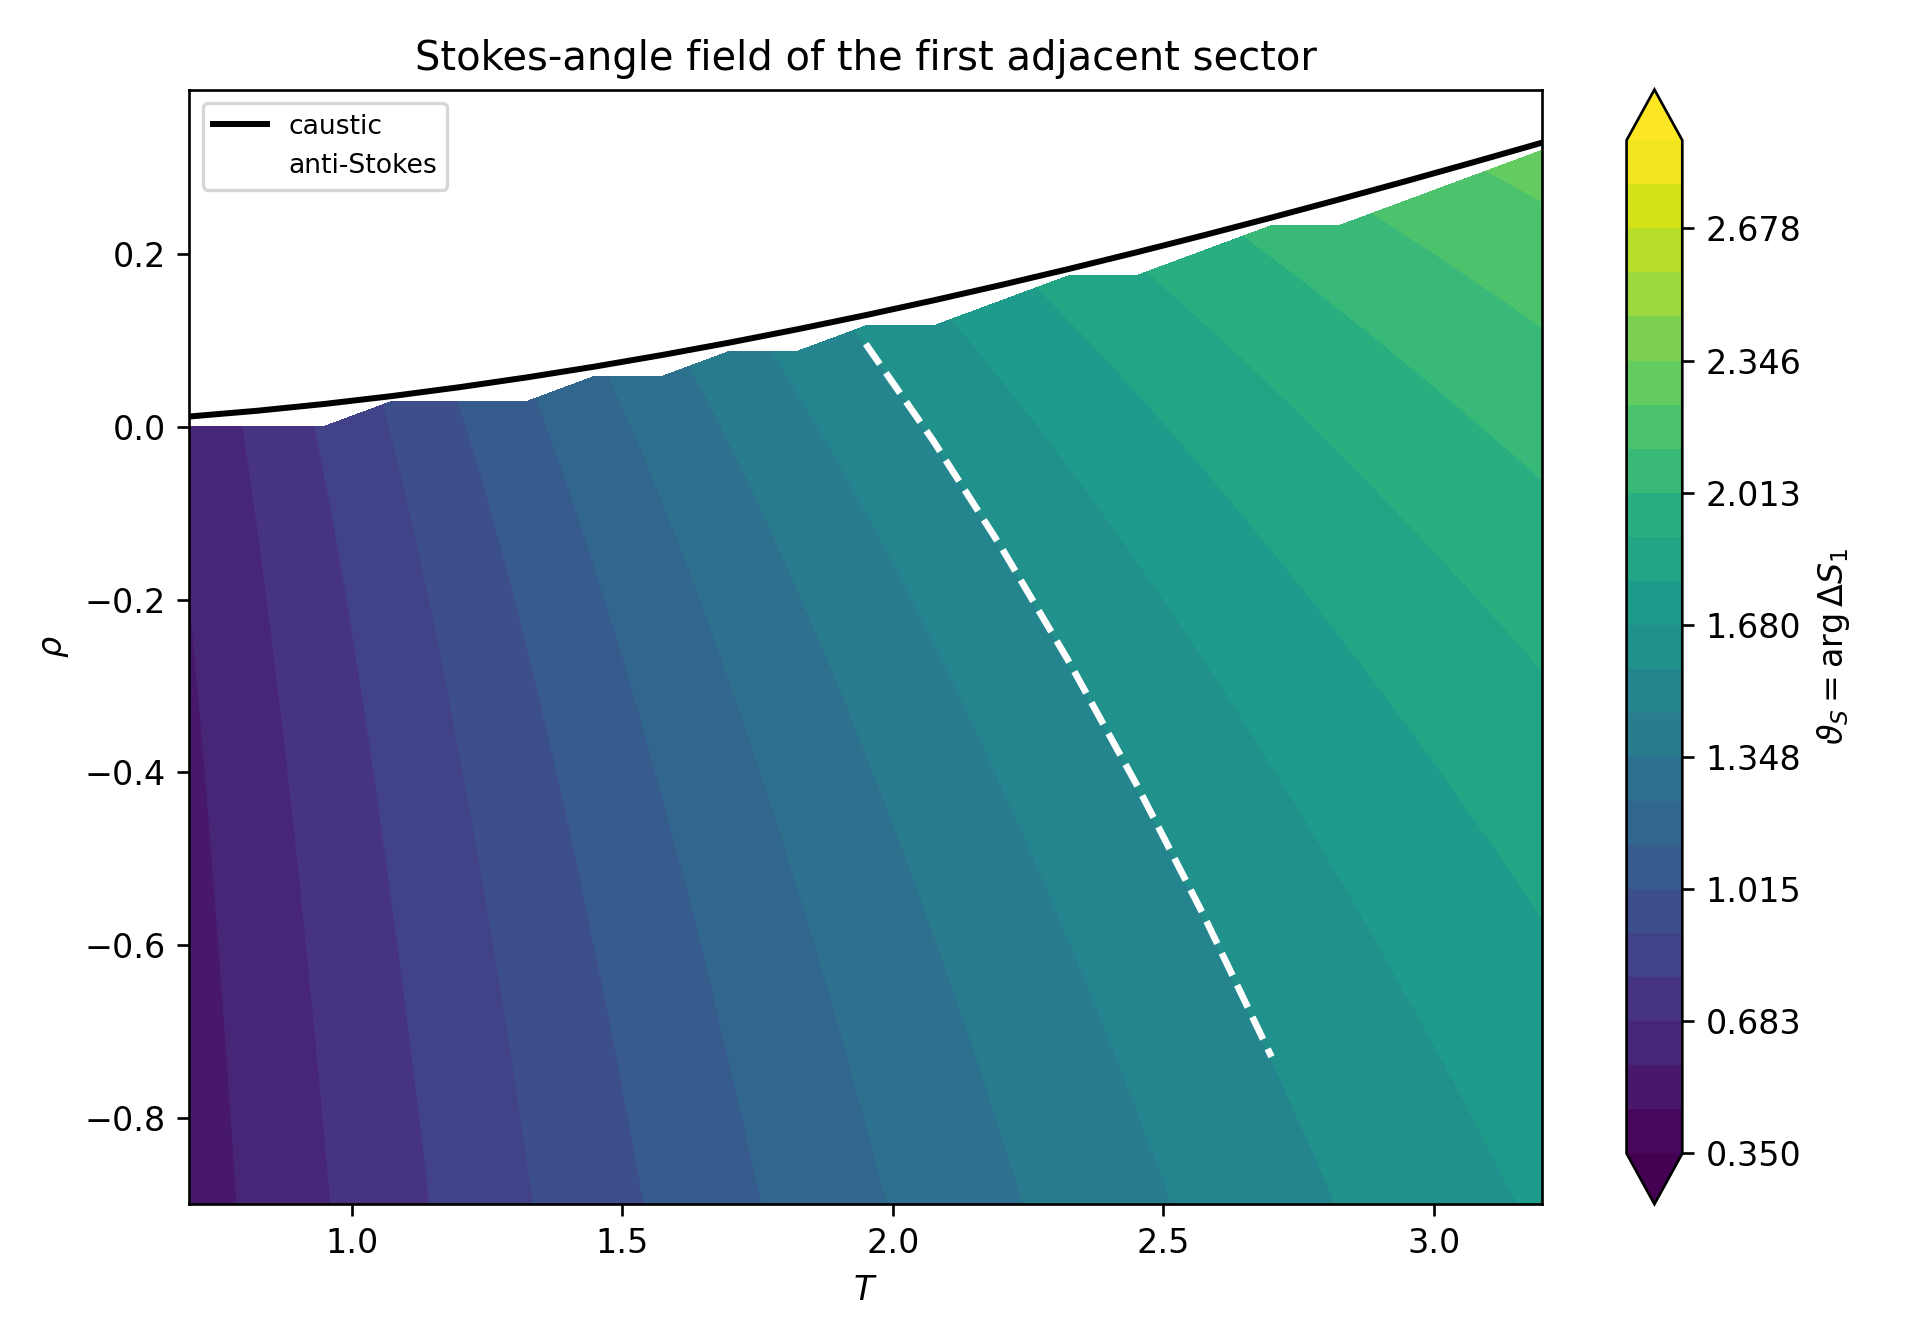
\includegraphics[width=0.86\textwidth]{../figures/heston_T_rho_stokes_angle.png}
\caption{Stokes-ray angle $\vartheta_S=\arg\Delta S_1$ across the two-dimensional real-adjacent domain. The same caustic and anti-Stokes boundaries are superposed.}
\label{fig:2dstokes}
\end{figure}

The resulting picture is an atlas rather than a single global transseries.  Away from boundaries, the two-sector basis deforms smoothly.  At the fold, the basis must be uniformised by Airy functions.  At the anti-Stokes curve, exponential dominance exchanges.  Moment-pole rearrangements additionally make root labels unreliable, which is why the pole-interval definition of the adjacent sector is used in the global scan.  A fully global construction beyond the caustic will require simultaneous tracking of complex saddles, moment-pole sheets and their Lefschetz thimbles.


\section{Post-caustic complex saddles and Airy Stokes matrices}
\label{sec:postcaustic}
The fold analysis above establishes the correct local scaling, but it does not by itself identify how the two adjacent saddle sectors should be continued on the full logarithmic Riemann surface.  This distinction matters because the affine closed form contains a logarithm: after the two real adjacent stationary points coalesce, a naive principal-branch evaluation makes the two complex actions appear simply conjugate, whereas analytic continuation from the pre-caustic sheet requires a non-trivial logarithmic lift.

\subsection{Full-sheet lift of the complex saddle pair}
Write
\begin{equation}
 M:=2\pi\frac{\kappa\theta}{\xi^2}.
 \label{eq:Mmonodromy}
\end{equation}
Before the fold the first two stationary points between the first two negative moment poles are real, $p_1>p_2$, and their singulants have the form
\begin{equation}
 \Delta S_j=A_j+\ii M,
 \qquad j=1,2.
 \label{eq:precausticpair}
\end{equation}
At the caustic $A_1=A_2$.  For $\rho>\rho_c$ the roots continue as
\begin{equation}
 p_\pm=\bar p\pm\ii y,
 \end{equation}
with $p_+$ the analytic continuation of the less-negative real root.  On the principal branch their singulants take the conjugate form
\begin{equation}
 \Delta S_+^{\rm pr}=A+\ii(M+\delta),
 \qquad
 \Delta S_-^{\rm pr}=A-\ii(M+\delta).
 \label{eq:principalpostpair}
\end{equation}
The full logarithmic monodromy of the affine exponent is $2\ii M=4\pi\ii\kappa\theta/\xi^2$.  Therefore the lower saddle must be lifted by one full logarithmic turn,
\begin{equation}
 \boxed{
 \Delta S_-^{\rm lift}
 =\Delta S_-^{\rm pr}+2\ii M
 =A+\ii(M-\delta).
 }
 \label{eq:sheetlift}
\end{equation}
The two analytically continued actions are consequently centred on the same monodromy level,
\begin{equation}
 \boxed{
 \operatorname{Im}\frac{\Delta S_+^{\rm pr}+\Delta S_-^{\rm lift}}{2}=M.
 }
 \label{eq:centeredmonodromy}
\end{equation}
In the numerical continuation this identity holds to machine precision throughout the tested post-caustic strip.  It also survives cross-maturity checks at $T=0.8,1,1.5,2$, evaluated at $\rho=\rho_c(T)+0.03$.

Figure~\ref{fig:postsaddles} shows the corresponding continuation of the two stationary points.  Their real parts meet at the fold while their imaginary parts split continuously with opposite signs.

\begin{figure}[H]
\centering
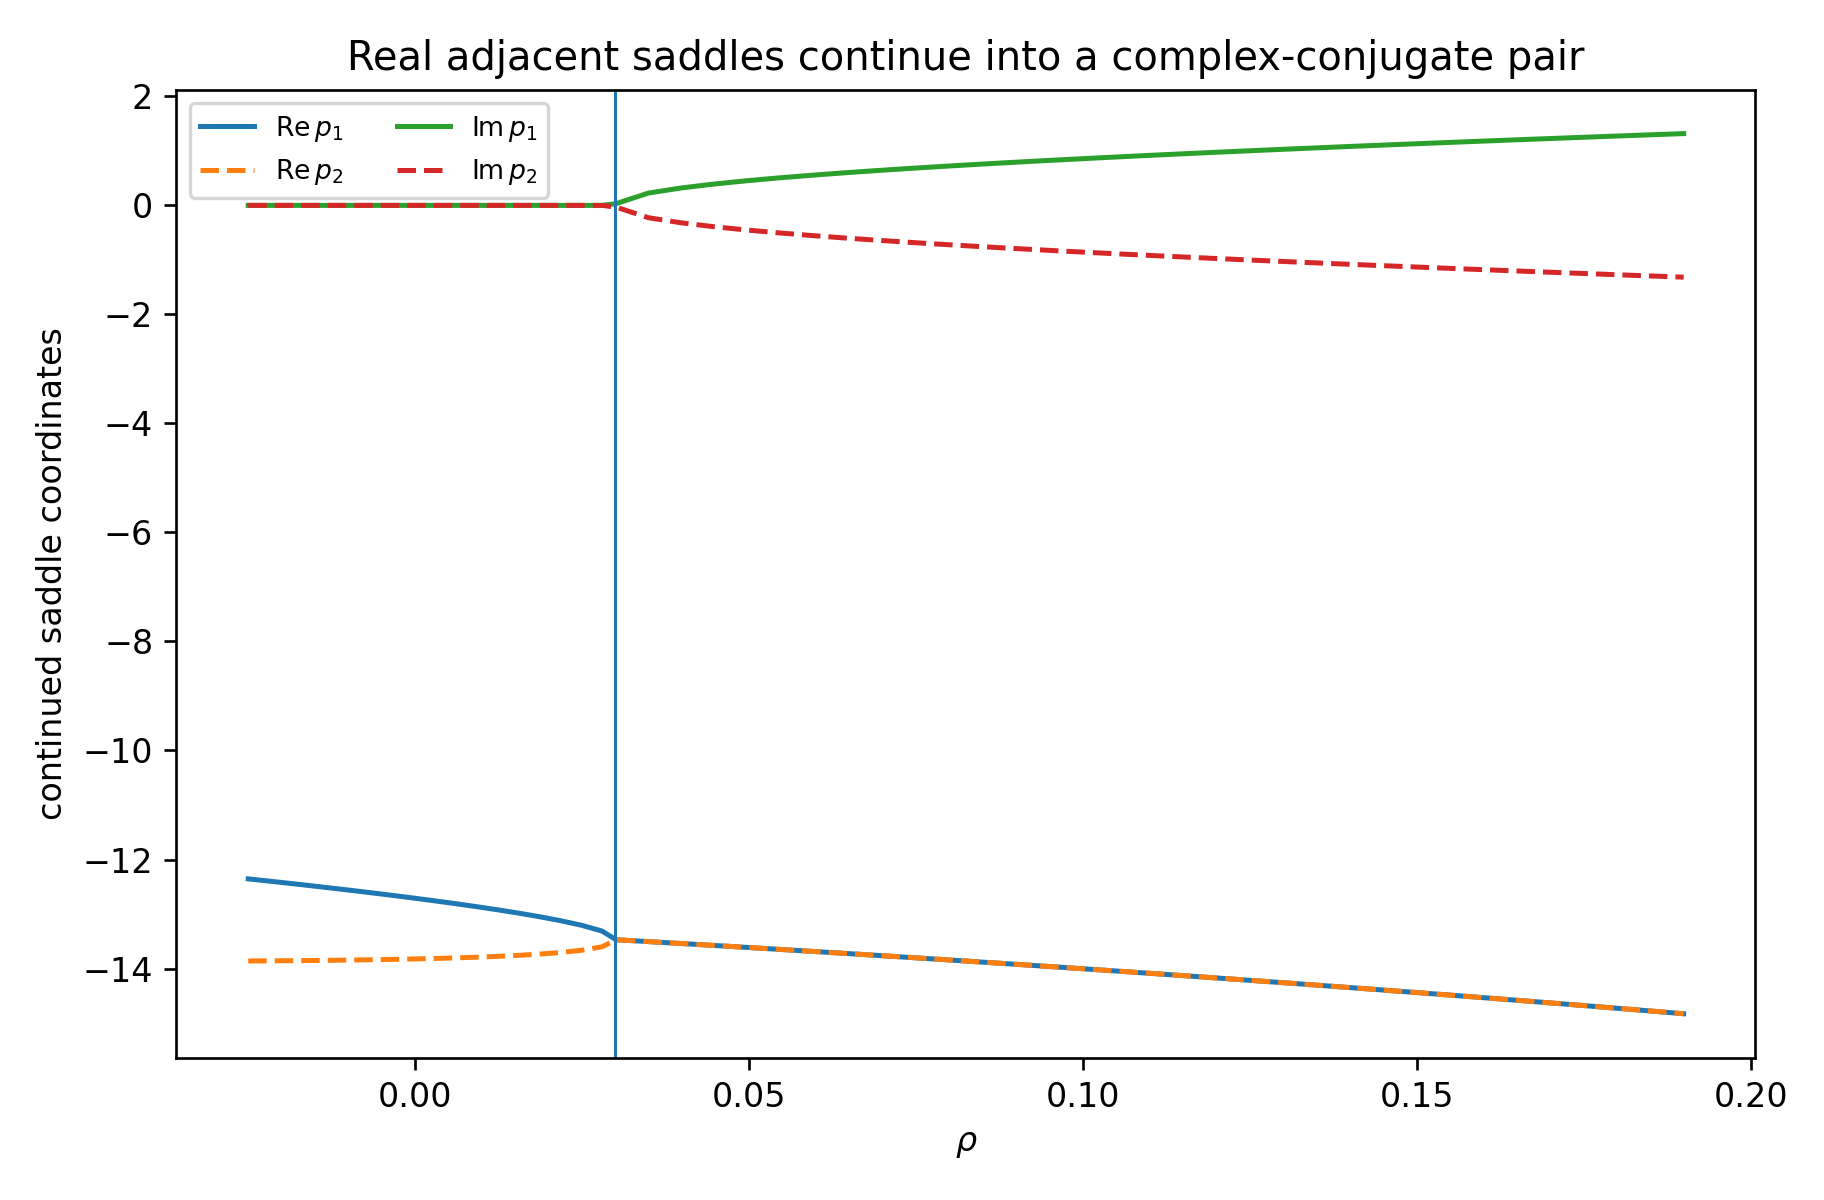
\includegraphics[width=0.84\textwidth]{../figures/heston_postcaustic_saddle_continuation.png}
\caption{Continuation of the first two adjacent stationary points through the correlation fold.  Two real roots coalesce at $\rho_c$ and continue as a complex-conjugate pair in the $p$ plane.}
\label{fig:postsaddles}
\end{figure}

The lifted actions behave differently from their principal-branch projections.  As shown in Fig.~\ref{fig:postactions}, the two same-sheet imaginary parts split about the fixed value $M$, rather than about zero.

\begin{figure}[H]
\centering
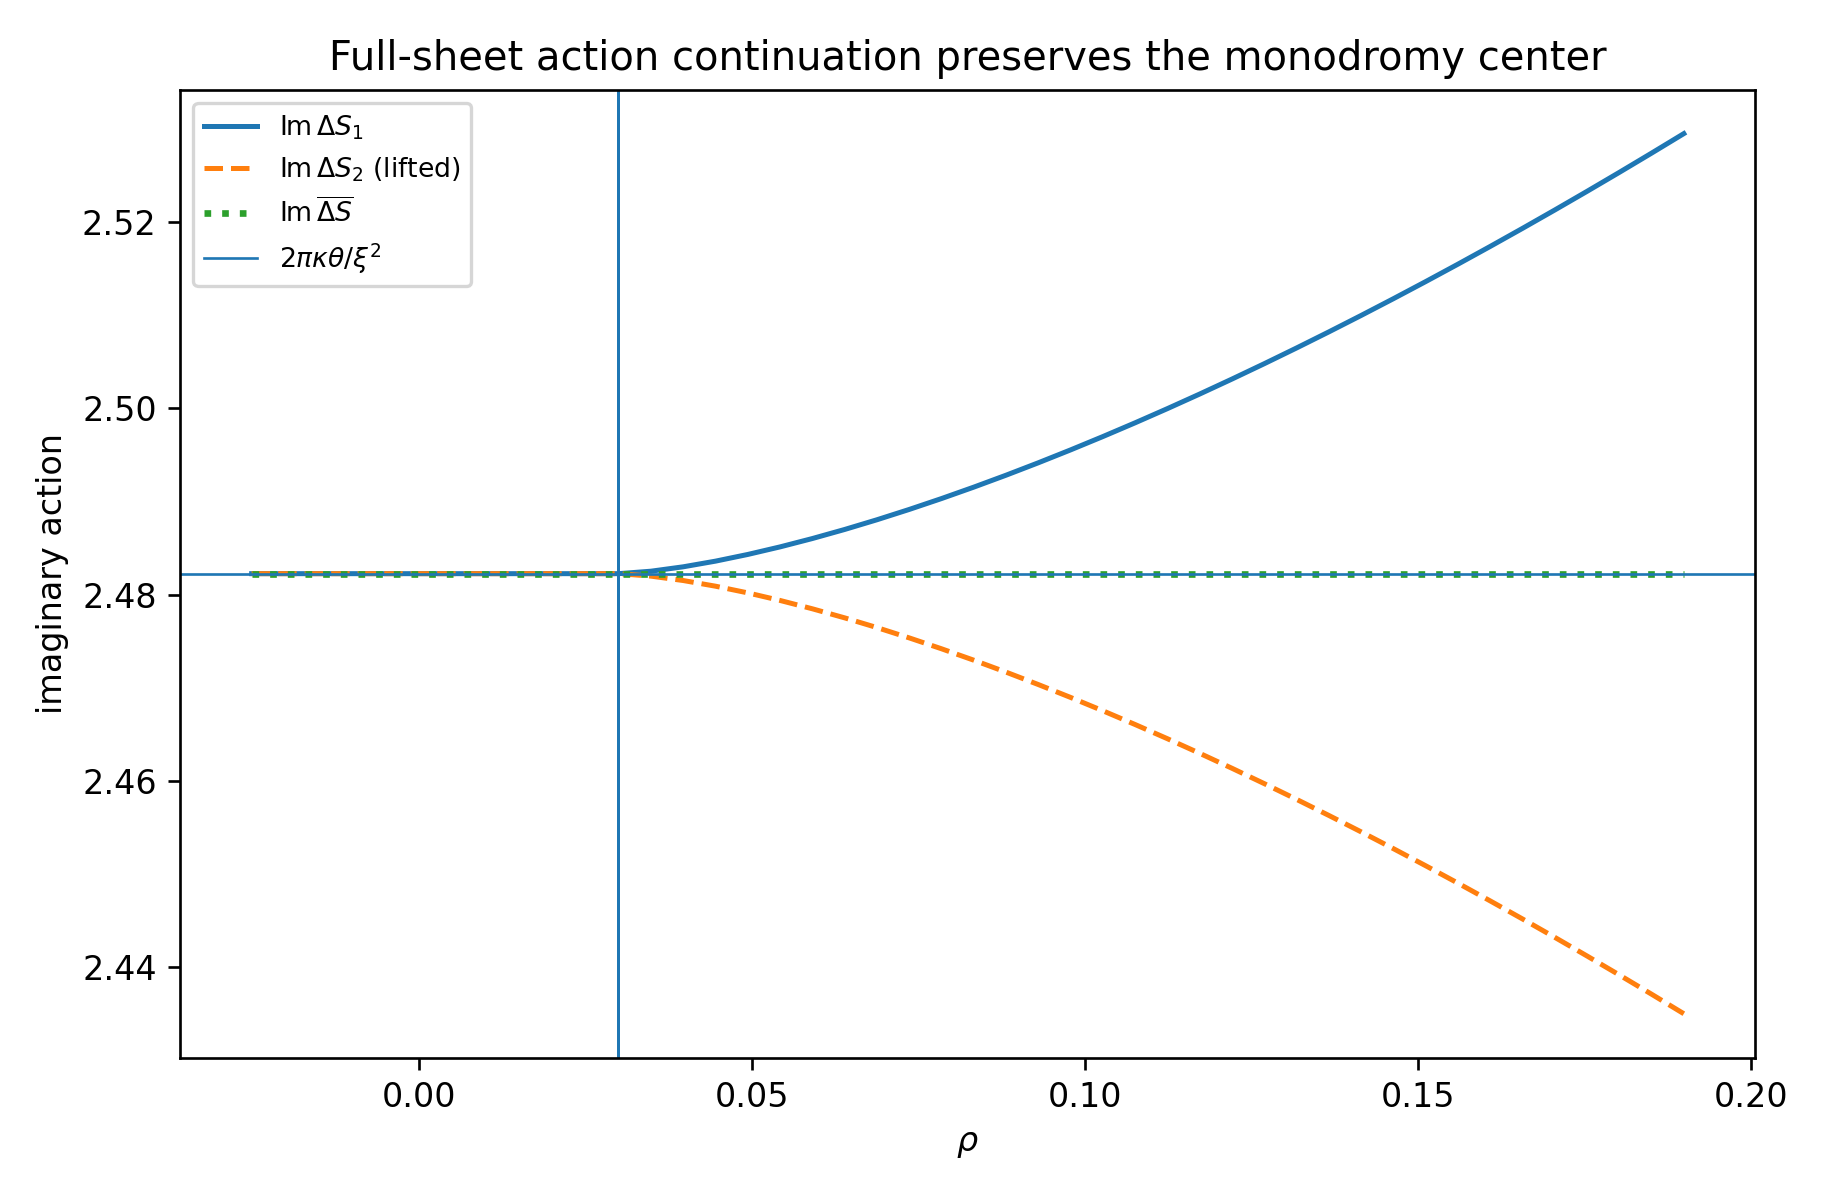
\includegraphics[width=0.84\textwidth]{../figures/heston_postcaustic_lifted_actions.png}
\caption{Imaginary parts of the two analytically continued adjacent actions on one logarithmic sheet.  Their average remains exactly at the monodromy centre $M=2\pi\kappa\theta/\xi^2$.}
\label{fig:postactions}
\end{figure}

\subsection{An exact CFU coordinate reconstructed from the two actions}
The Chester--Friedman--Ursell construction replaces two coalescing saddles by the cubic normal form \citep{chester1957}
\begin{equation}
 \Phi=A+\frac{u^3}{3}-\zeta u.
 \label{eq:cfunormalglobal}
\end{equation}
The two critical points $u_\pm=\pm\sqrt{\zeta}$ have phase difference proportional to $\zeta^{3/2}$.  With our saddle labelling it is convenient to define the exact control coordinate by
\begin{equation}
 \boxed{
 \frac{4}{3}\,\zeta_{\rm CFU}^{3/2}
 =\Delta S_2-\Delta S_1,
 }
 \label{eq:exactcfuzeta}
\end{equation}
where the branch is chosen continuously so that $\zeta_{\rm CFU}>0$ on the two-real-saddle side.  This branch becomes real and negative after the fold.  Hence the same variable describes both regimes:
\begin{align}
 \zeta_{\rm CFU}>0
 &\quad\Longleftrightarrow\quad
 \text{two real adjacent saddles},\\
 \zeta_{\rm CFU}<0
 &\quad\Longleftrightarrow\quad
 \text{complex-conjugate adjacent saddles}.
\end{align}
The construction is not merely local.  Close to the fold it reduces to the derivative-based coordinate derived earlier,
\begin{equation}
 \zeta_{\rm CFU}
 =-1.09326849050\,(\rho-\rho_c)+O((\rho-\rho_c)^2).
\end{equation}
For $|\rho-\rho_c|<0.02$ the numerical exact-action coordinate and the linear normal form differ by at most about $0.33\%$, while the post-caustic imaginary part of $\zeta_{\rm CFU}$ remains below $2.1\times10^{-17}$.  Figure~\ref{fig:cfuglobal} displays the continuation.

\begin{figure}[H]
\centering
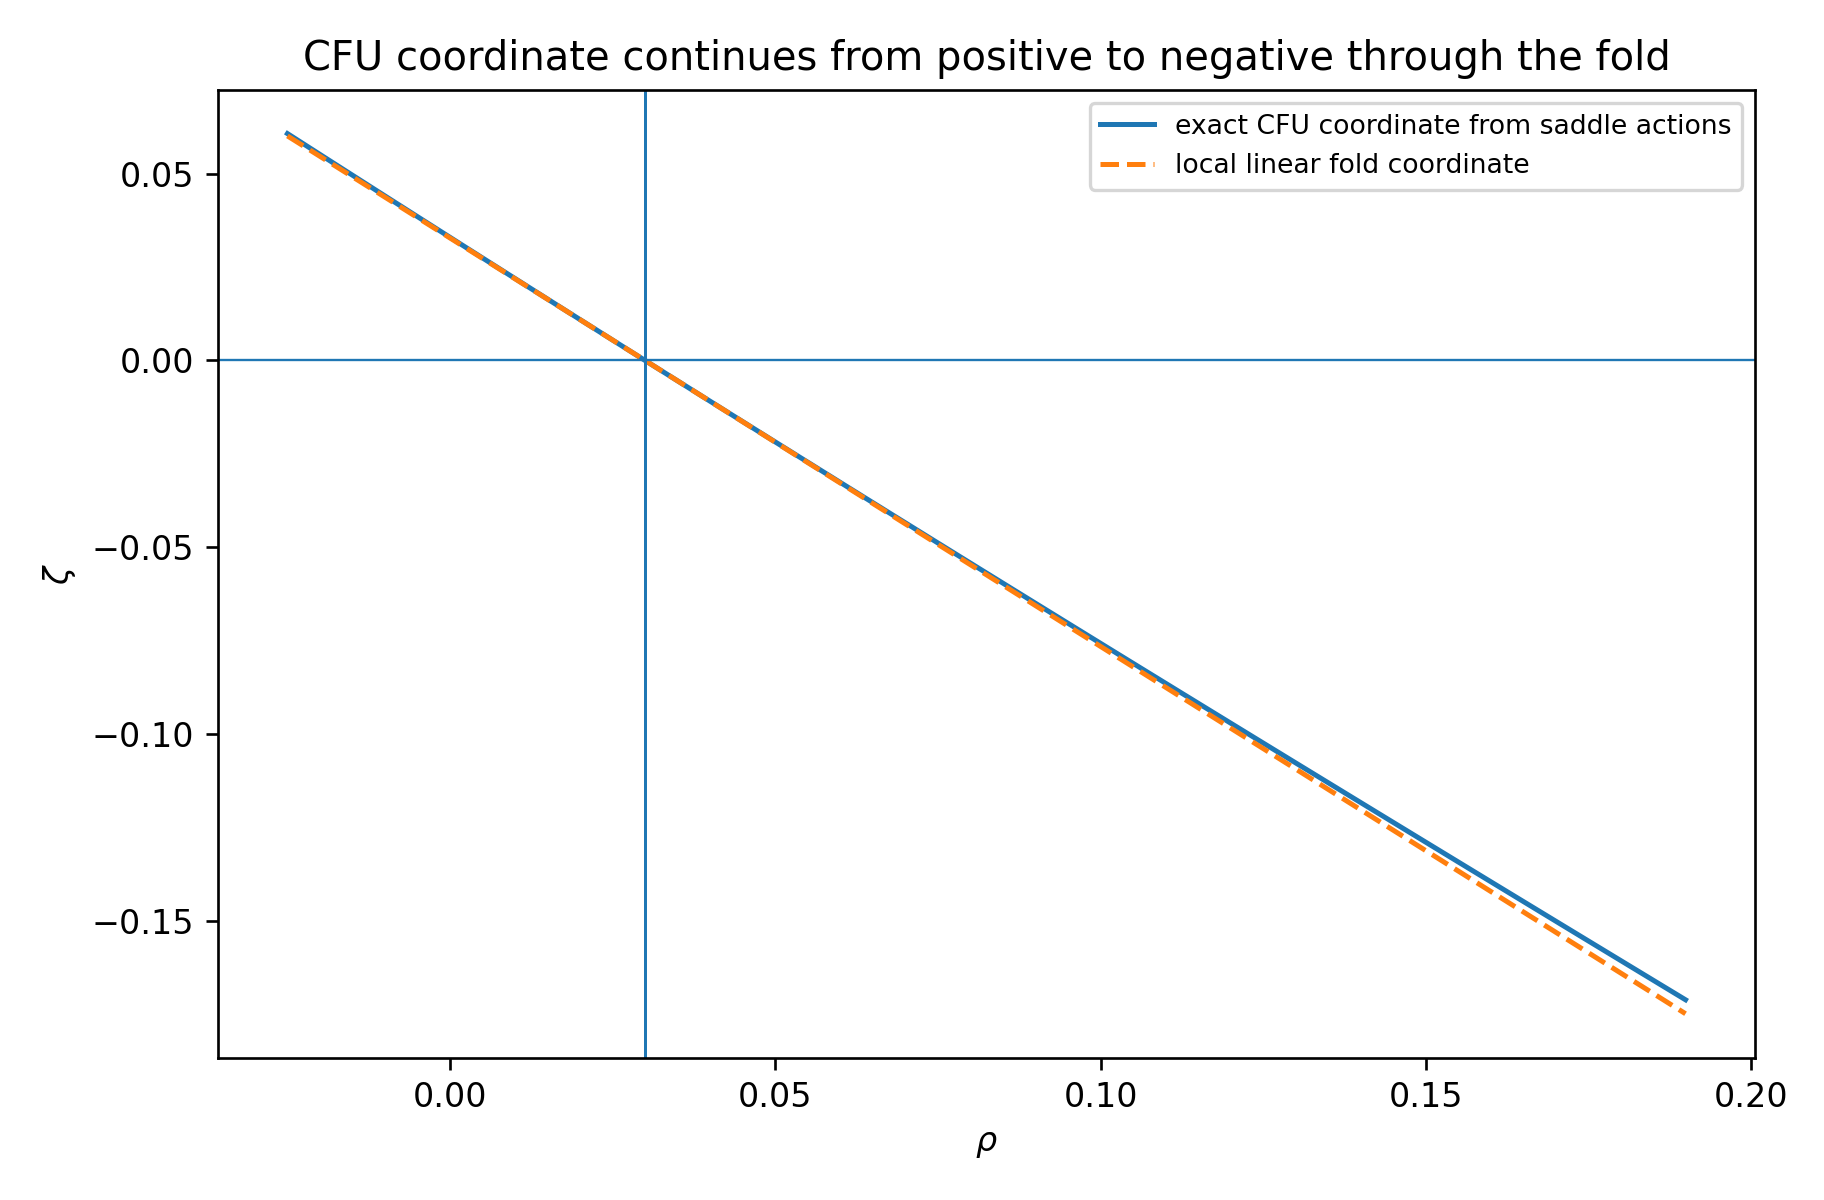
\includegraphics[width=0.84\textwidth]{../figures/heston_cfu_coordinate_through_fold.png}
\caption{The exact CFU coordinate reconstructed from the two saddle actions.  It is positive before the fold, vanishes at coalescence and becomes negative when the stationary points form a complex pair.}
\label{fig:cfuglobal}
\end{figure}

\subsection{Airy connection matrices and the reorganisation of saddle sectors}
A simple turning point has universal Airy Stokes data.  In a standard WKB basis ordered by the two local exponentials, elementary crossings can be represented by the alternating triangular matrices \citep{fujimori2025}
\begin{equation}
 S_{\rm U}^{\rm WKB}
 =\begin{pmatrix}1&\ii\\0&1\end{pmatrix},
 \qquad
 S_{\rm L}^{\rm WKB}
 =\begin{pmatrix}1&0\\\ii&1\end{pmatrix}.
 \label{eq:airywkbmatrices}
\end{equation}
After absorbing the Gaussian orientation phases into the definition of the oriented thimble integrals, the same local wall crossing is represented by integer unipotent Picard--Lefschetz matrices,
\begin{equation}
 S_{\rm U}^{\rm th}
 =\begin{pmatrix}1&1\\0&1\end{pmatrix},
 \qquad
 S_{\rm L}^{\rm th}
 =\begin{pmatrix}1&0\\1&1\end{pmatrix}.
 \label{eq:airythimblematrix}
\end{equation}
The sign of an off-diagonal entry changes if a thimble orientation is reversed; the invariant content is the unit intersection number.  This is precisely why the local Airy matrices should not be confused with the previously measured global Heston value $S_{01}=-1$: the latter includes the orientation of the physical Bromwich contour and the choice of the adjacent Heston thimble.  The Airy model supplies the universal local basis change at the fold, whereas the global contour fixes the Heston sign.  This local/global distinction is also the natural language for comparing Picard--Lefschetz and resurgent Stokes data \citep{li2026}.

The connection can also be read directly from the standard Airy asymptotics \citep{dlmf2026}.  If $Z>0$,
\begin{equation}
 \operatorname{Ai}(Z)\sim \frac{1}{2\sqrt{\pi}Z^{1/4}}
 \exp\!\left(-\frac23 Z^{3/2}\right),
 \label{eq:airyoneexp}
\end{equation}
so the uniform block re-expands into one decaying real-saddle exponential.  If $Z=-X<0$,
\begin{equation}
 \operatorname{Ai}(-X)\sim \frac{1}{\sqrt{\pi}X^{1/4}}
 \sin\!\left(\frac23 X^{3/2}+\frac{\pi}{4}\right),
 \label{eq:airytwoexp}
\end{equation}
which is the coherent sum of two complex-conjugate exponentials.  Thus the Airy connection matrix is not merely a formal change of basis: it is the asymptotic rule converting the two-real-saddle chart into the complex-pair chart through one uniform function.  With $\varepsilon=0.004$, the leading formulas \eqref{eq:airyoneexp}--\eqref{eq:airytwoexp} reproduce the exact canonical Airy block with a maximum envelope-normalized error of $1.25\%$ for $|Z|\ge4$ in the numerical test shown in Fig.~\ref{fig:postairymatch}.

\begin{figure}[H]
\centering
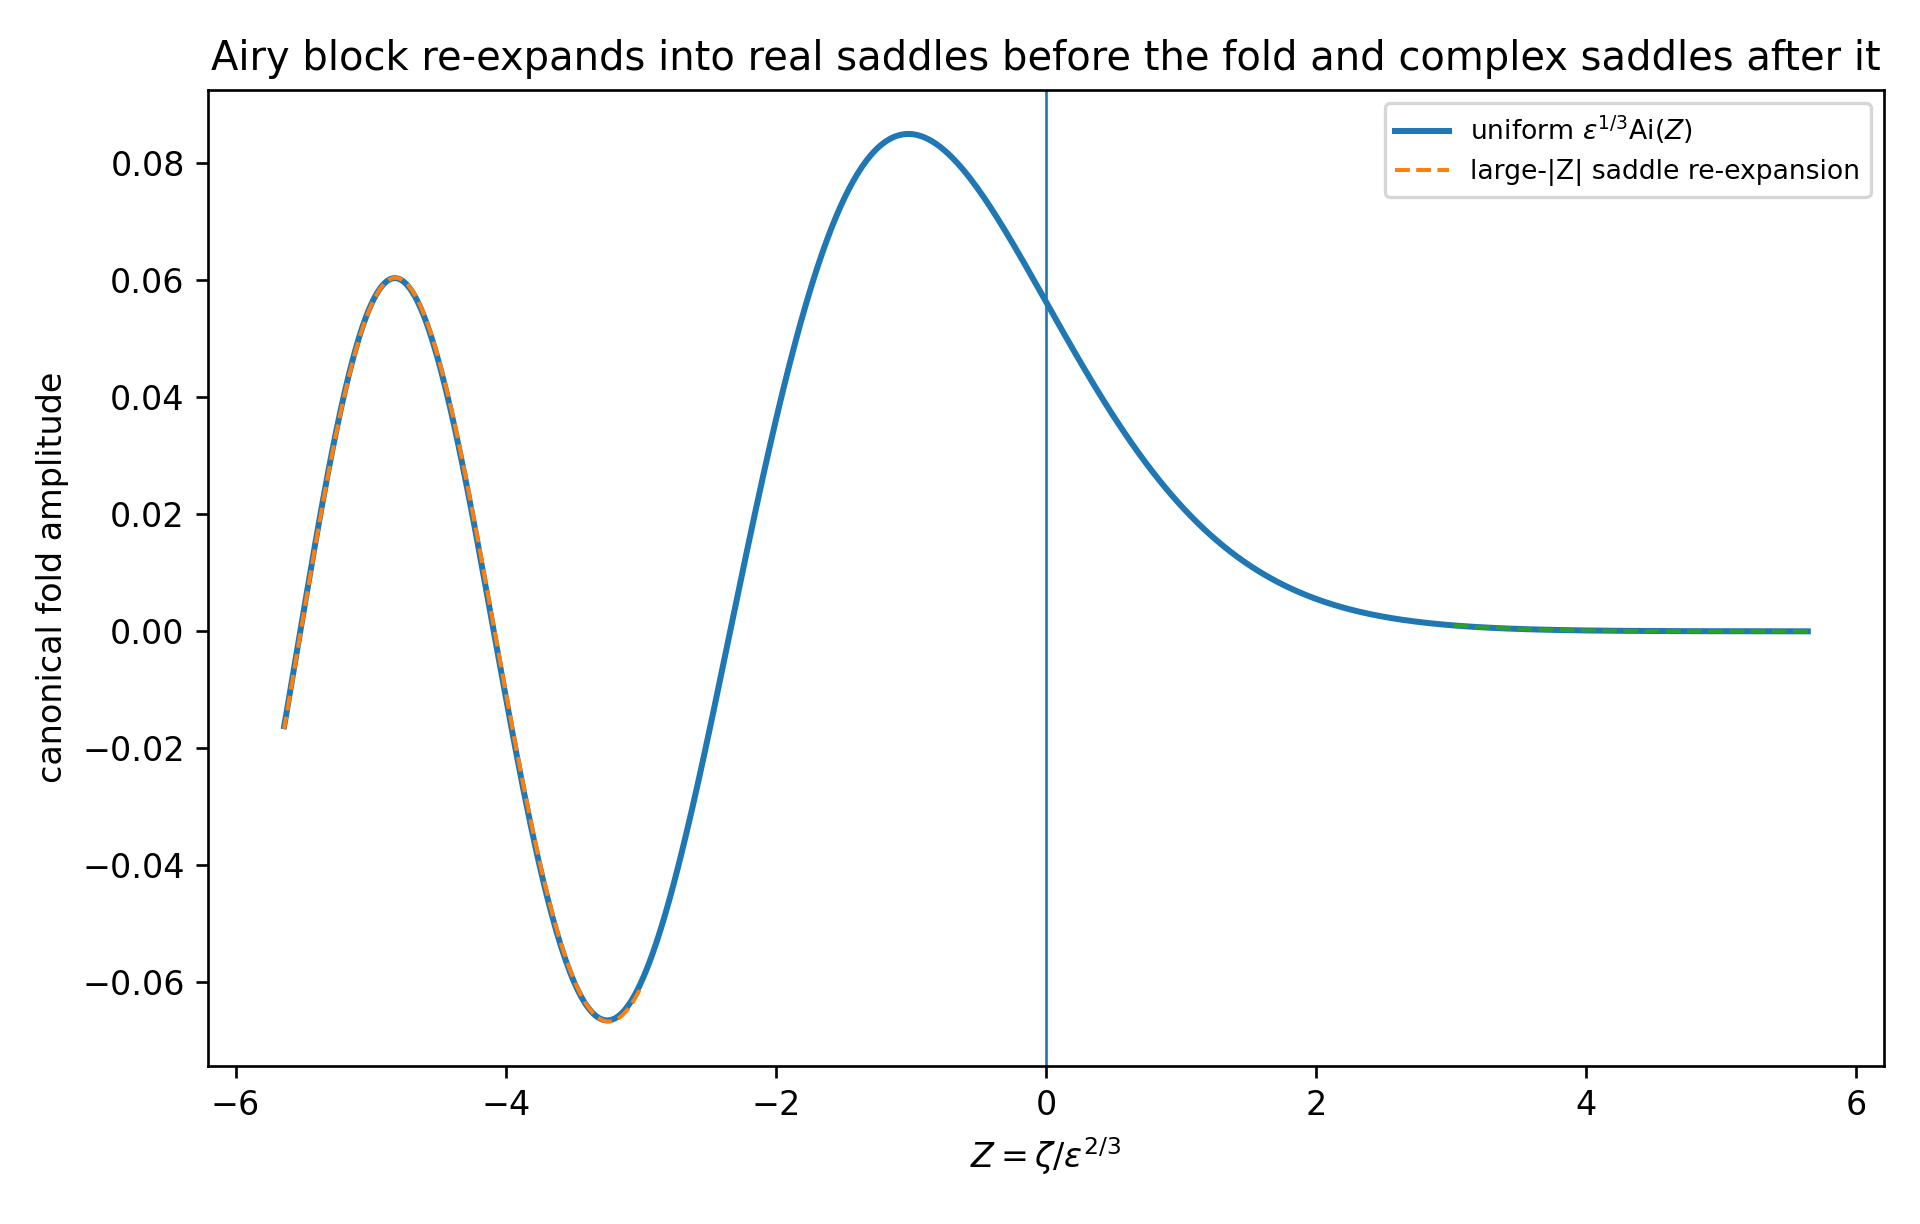
\includegraphics[width=0.86\textwidth]{../figures/heston_postcaustic_airy_matching.png}
\caption{Uniform Airy block and its large-$|Z|$ saddle re-expansion.  For $Z>0$ the asymptotic form contains one decaying real-saddle exponential; for $Z<0$ it is the interference of two complex-conjugate saddle exponentials.  The central region is intentionally left to the exact Airy block, where separate saddle asymptotics are non-uniform.}
\label{fig:postairymatch}
\end{figure}

The consequence is that the separate Gaussian sectors attached to $p_1$ and $p_2$ cease to be a good basis inside the $O(\varepsilon^{2/3})$ fold layer.  They are replaced by one uniform Airy block.  On the complex-saddle side the same Airy block can again be expanded into two saddle contributions.  Thus the fold does not destroy the adjacent non-perturbative information; it reorganises it through a universal unipotent connection matrix, dressed by the analytic Heston amplitude multiplying $\operatorname{Ai}$ and $\operatorname{Ai}'$.

\subsection{Local fluctuation sectors after the caustic}
The post-caustic continuation should preserve more than the stationary-point locations.  We therefore expand independently about both complex saddles at $\rho=0.05$.  Choosing local steepest coordinates $a_\pm$ such that
\begin{equation}
 a_\pm^2\Lambda''(p_\pm)=-1,
\end{equation}
the normalized local sectors take the form
\begin{equation}
 \Phi_\pm(\varepsilon)=1+d_1^{(\pm)}\varepsilon+d_2^{(\pm)}\varepsilon^2+\cdots.
\end{equation}
For real Heston parameters the projected saddles are conjugate, so analyticity predicts
\begin{equation}
 d_n^{(-)}=\overline{d_n^{(+)}}.
 \label{eq:complexfluctconj}
\end{equation}
The direct Cauchy-Taylor calculation satisfies \eqref{eq:complexfluctconj} to the stored numerical precision through the first six coefficients.  For example,
\begin{equation}
 d_1^{(+)}=-2.87635671842+32.1669377615\,\ii,
 \qquad
 d_1^{(-)}=\overline{d_1^{(+)}}.
\end{equation}
The rapid growth of these coefficients close to the caustic is expected: isolated complex-saddle expansions become badly conditioned inside the same $O(\varepsilon^{2/3})$ region in which the Airy block is the correct basis.  Their exact conjugacy nevertheless provides a sector-level check that the post-caustic roots and their local fluctuations are being followed consistently.

\subsection{Projected complex saddles in the physical Borel plane}
There is a useful distinction between the lifted logarithmic cover and the Borel plane of the physical perturbative series.  Since the physical fluctuation coefficients are real, their Borel singularities occur in conjugate pairs.  The relevant projected locations are therefore the principal representatives
\begin{equation}
 \Delta S_+^{\rm pr},
 \qquad
 \overline{\Delta S_+^{\rm pr}},
\end{equation}
not the two same-sheet lifts in Eq.~\eqref{eq:sheetlift}.  This is a projection of the logarithmic cover onto the principal Borel plane, not a contradiction of the full-sheet continuation.

We test this independently at $\rho=0.04,0.05,0.08$, all beyond $\rho_c$.  With only 32 physical-saddle fluctuation coefficients the nearest conformal--Pad\'e pole is within $5.99\%$, $5.88\%$ and $6.27\%$, respectively, of the predicted projected complex action.  A second diagnostic fits the late conformal-Borel coefficients directly to the expected conjugate logarithmic pair, without fixing the singulant.  Using orders 20--31 gives relative location discrepancies $1.93\%$, $1.33\%$ and $1.45\%$, respectively.  These errors are larger than at the 75-coefficient benchmark, as expected near a coalescence where two singularities compete, but the late perturbative coefficients quantitatively track the complex continuation without using the saddle positions in their generation.

\begin{figure}[H]
\centering
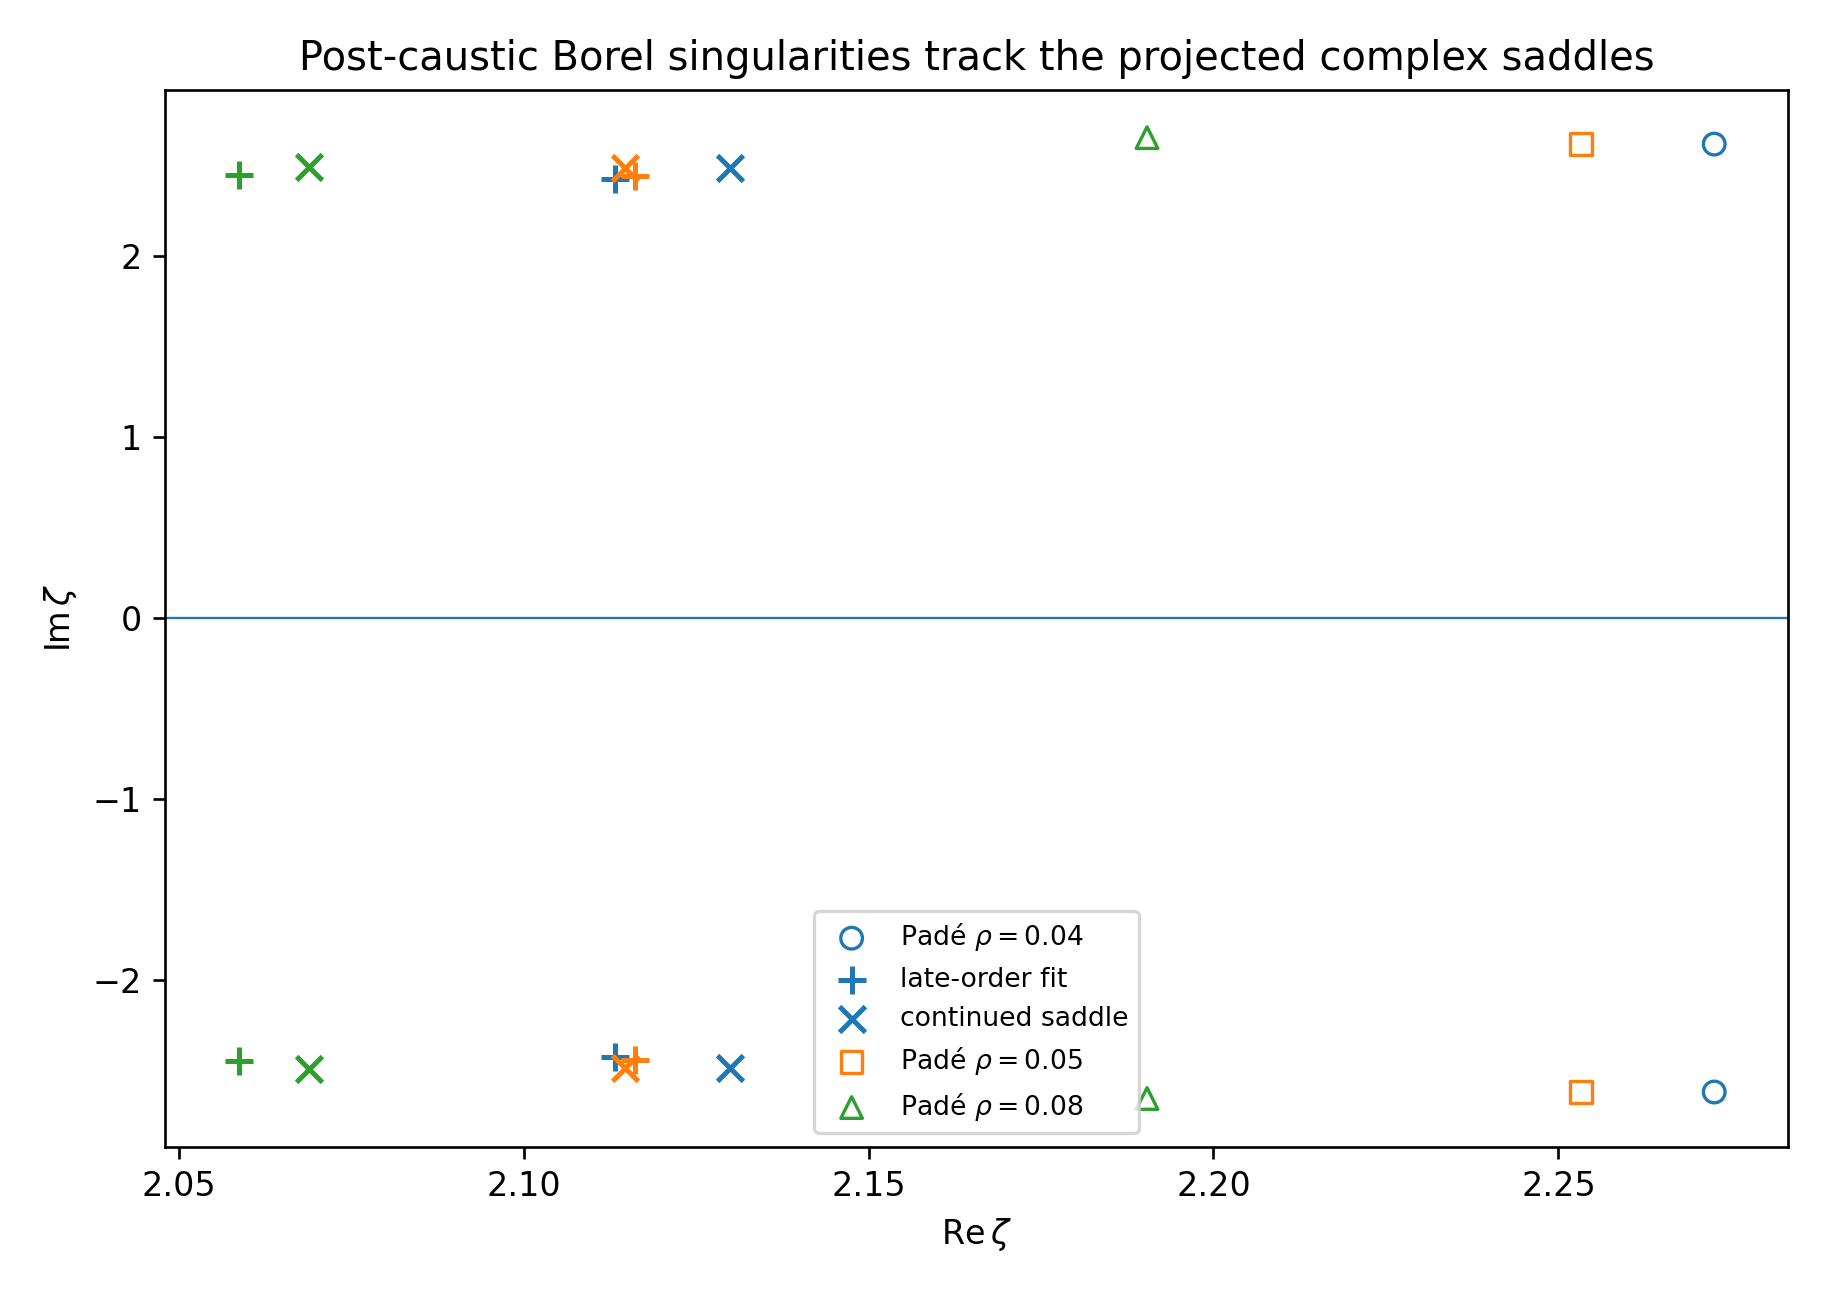
\includegraphics[width=0.84\textwidth]{../figures/heston_postcaustic_borel_pair.png}
\caption{Post-caustic Borel check.  Crosses mark the independently continued principal complex saddle actions, open markers show the nearest conformal--Pad\'e singularities from 32 physical-sector coefficients, and plus signs show the independent late-order conjugate-pair fits.  Reality of the perturbative series produces the conjugate pair.}
\label{fig:postborel}
\end{figure}

The combined picture is therefore coherent on three levels.  The $p$-plane saddles continue from real to complex; their \emph{lifted} actions form a same-sheet Airy pair centred on the exact logarithmic monodromy; and their \emph{projected} principal representatives are visible as conjugate singularities in the physical Borel plane.  This is the required continuation of the adjacent resurgent sector beyond the fold.


\section{Results summary}
Table~\ref{tab:results} collects the headline quantities used to support the main claims.  Detailed convergence tables and parameter sweeps are provided by the repository outputs described in Section~\ref{sec:repro}.

\begin{table}[H]
\centering
\small
\begin{tabular}{ll}
\toprule
Quantity & Value \\
\midrule
Physical saddle $p_\star$ & $-2.849561078040$ \\
Affine rate $I(x_\star)$ & $0.396018751741$ \\
Independent Hamiltonian action & $0.396018650224$ \\
Leading large-order Borel estimate & $-0.396018496470$ \\
Maximum Borel--Pad\'e tail error & $1.85\times10^{-4}$ \\
Adjacent-sheet saddle $p_1$ & $-7.998322139804$ \\
Adjacent singulant $\Delta S_1$ & $2.792240162467\pm2.482246047281\,\ii$ \\
75-coefficient late-order singulant gap & $0.328\%$ \\
Direct lateral Stokes multiplier & $-0.998565810+0.001484197\,\ii$ \\
Picard--Lefschetz connection integer & $S_{01}=-1$ \\
Correlation fold $(\rho_c,p_c)$ & $(0.0299495156775,-13.4709103772980)$ \\
Maturity anti-Stokes crossing $T_A$ & $2.678155844206$ \\
Mean-reversion anti-Stokes crossing $\kappa_A$ & $5.470788617678$ \\
2D $(T,\rho)$ atlas points & $763$ \\
Post-caustic late-order location error, max & $1.93\%$ \\
Airy saddle re-expansion error for $|Z|\ge4$ & $1.25\%$ \\
\bottomrule
\end{tabular}
\caption{Selected benchmark and continuation results.  Errors are numerical diagnostics for the parameter choices stated in the text; they are not theorem-level error bounds.}
\label{tab:results}
\end{table}

\section{Conclusions}
For the small-noise Heston left-tail observable studied here, several independent calculations select the same non-perturbative structures.  At the benchmark point, the affine saddle and the Freidlin--Wentzell Hamiltonian problem agree on the leading rate, and the perturbative large-order coefficients recover the corresponding Borel scale.  Borel--Pad\'e resummation materially extends the useful range of the asymptotic expansion.

The first adjacent logarithmic sheet provides a more stringent resurgent test.  Its independently continued action is recovered from high-order coefficients, its local fluctuation series reproduces the reduced lateral jump, and a direct Borel discontinuity gives a Stokes multiplier numerically indistinguishable from $-1$ at the quoted resolution.  Picard--Lefschetz flow then supplies the geometric explanation: the relevant oriented intersection number jumps from $0$ to $-1$ across the Stokes wall.

This structure persists under parameter continuation until ordinary saddle coordinates cease to be uniform.  The imaginary part of the adjacent action follows the logarithmic monodromy $2\pi\kappa\theta/\xi^2$, while the thimble connection integer remains constant on the tested nondegenerate component.  The continuation also identifies where the local transseries basis must change: a correlation fold coalesces the adjacent saddles, and anti-Stokes curves exchange their exponential hierarchy.  The fold is resolved by a uniform Airy description; beyond it, the two complex saddles, their lifted actions, their local fluctuation sectors, and their projected Borel singularities continue consistently.

The appropriate interpretation is therefore a \emph{resurgent atlas} rather than a single global transseries.  On regular parameter domains, saddle sectors deform smoothly; at caustics they are replaced by uniform canonical blocks; across anti-Stokes boundaries the dominant exponential basis changes.  These statements are supported here by numerical asymptotics and contour geometry, not by a global theorem on the complete Heston Riemann surface.

\paragraph{Scope of the claim.}
The project establishes a reproducible benchmark and a coherent first continuation through one caustic.  It does not claim that financial markets are quantum systems, that all Heston observables are resurgent, or that renormalons have been identified in finance.  A global classification of moment-pole sheets, thimble endpoints, and all higher sectors is left as future work.

\appendix
\section{Relation between the Hamiltonian and affine saddle}
The scaled cumulant generator $\Lambda(p)$ is the endpoint Hamilton--Jacobi solution associated with the small-noise process. Legendre duality gives
\begin{equation}
 I(x)=\sup_p\{px-\Lambda(p)\}.
\end{equation}
At a differentiable point, the maximiser satisfies $\Lambda'(p_\star)=x$, which is exactly the affine saddle equation \eqref{eq:saddleeq}. In the pathwise formulation, the terminal Lagrange multiplier enforcing $x(T)=x$ is the conserved Hamiltonian momentum $p_x$. Consequently the equality
\begin{equation}
 p_x=p_\star
\end{equation}
is expected theoretically, while the equality of the minimized path action with $p_\star x-\Lambda(p_\star)$ is the contraction of the sample-path rate functional to the terminal log-return. The numerical agreement in \eqref{eq:affineres}--\eqref{eq:hamres} is therefore both a code validation and an explicit demonstration of the duality.

\section{Conformal-map geometry}
The map \eqref{eq:conformal} follows by uniformising a square-root cut. If
\begin{equation}
 u=\sqrt{1+\zeta/I},
\end{equation}
then the Cayley transformation
\begin{equation}
 w=\frac{u-1}{u+1}
\end{equation}
maps the right half of the $u$ plane to $|w|<1$. Solving for $u=(1+w)/(1-w)$ gives
\begin{equation}
 1+\frac{\zeta}{I}=\left(\frac{1+w}{1-w}\right)^2,
\end{equation}
and hence
\begin{equation}
 \zeta=\frac{4Iw}{(1-w)^2}.
\end{equation}
The leading cut is moved to $|w|=1$, while any secondary singularity not lying on that cut may appear inside the disk and become accessible to a new Pad\'e approximation.

\section{Falsification criteria for the secondary claim}
The adjacent-sheet interpretation should be rejected if any of the following occurs after extending the calculation:
\begin{enumerate}
 \item the conformal-Pad\'e pair drifts away from $w(\Delta S_1)$ as the coefficient count rises;
 \item the pair is unstable under reasonable changes of Pad\'e numerator/denominator degree;
 \item the local D-log exponent is incompatible with the independently calculated saddle fluctuation sector;
 \item a closer analytic obstruction is found whose singulant explains the residual poles more naturally;
 \item direct hyperasymptotic remainder analysis selects a different adjacent saddle.
\end{enumerate}
This explicit failure criterion is important: the project aims to test resurgence, not to fit every numerical feature to resurgent language.

\begin{thebibliography}{99}

\bibitem[Aniceto et~al.(2019)Aniceto, Basar, and Schiappa]{aniceto2019}
I.~Aniceto, G.~Basar, and R.~Schiappa.
\newblock A primer on resurgent transseries and their asymptotics.
\newblock {\em Physics Reports}, 809:1--135, 2019.
\newblock doi:10.1016/j.physrep.2019.02.003.

\bibitem[Baaquie(2002)]{baaquie2002}
B.~E. Baaquie.
\newblock Quantum field theory of forward rates with stochastic volatility.
\newblock {\em Physical Review E}, 65:056122, 2002.
\newblock doi:10.1103/PhysRevE.65.056122.

\bibitem[Berry and Howls(1991)]{berry1991}
M.~V. Berry and C.~J. Howls.
\newblock Hyperasymptotics for integrals with saddles.
\newblock {\em Proceedings of the Royal Society A}, 434(1892):657--675, 1991.
\newblock doi:10.1098/rspa.1991.0119.

\bibitem[Contreras and Hojman(2014)]{contreras2014}
M.~Contreras and S.~A. Hojman.
\newblock Option pricing, stochastic volatility, singular dynamics and constrained path integrals.
\newblock {\em Physica A}, 393:391--403, 2014.
\newblock doi:10.1016/j.physa.2013.08.057.

\bibitem[Geha et~al.(2024)Geha, Jacquier, and \v{Z}uri\v{c}]{geha2024}
M.~Geha, A.~Jacquier, and \v{Z}.~\v{Z}uri\v{c}.
\newblock Large and moderate deviations for importance sampling in the Heston model.
\newblock {\em Annals of Operations Research}, 336:47--92, 2024.
\newblock doi:10.1007/s10479-023-05424-0.

\bibitem[Heston(1993)]{heston1993}
S.~L. Heston.
\newblock A closed-form solution for options with stochastic volatility with applications to bond and currency options.
\newblock {\em The Review of Financial Studies}, 6(2):327--343, 1993.
\newblock doi:10.1093/rfs/6.2.327.

\bibitem[Keller-Ressel(2011)]{kellerressel2011}
M.~Keller-Ressel.
\newblock Moment explosions and long-term behavior of affine stochastic volatility models.
\newblock {\em Mathematical Finance}, 21(1):73--98, 2011.
\newblock doi:10.1111/j.1467-9965.2010.00423.x.

\bibitem[Pham(1983)]{pham1983}
F.~Pham.
\newblock Vanishing homologies and the $n$ variable saddlepoint method.
\newblock In {\em Singularities, Part 2}, Proceedings of Symposia in Pure Mathematics, volume 40, pages 319--333. American Mathematical Society, 1983.
\newblock doi:10.1090/pspum/040.2/713258.

\bibitem[Witten(2011)]{witten2011}
E.~Witten.
\newblock Analytic continuation of Chern--Simons theory.
\newblock In {\em Chern--Simons Gauge Theory: 20 Years After}, AMS/IP Studies in Advanced Mathematics, volume 50, pages 347--446. American Mathematical Society, 2011.
\newblock doi:10.1090/amsip/050/19.

\bibitem[Chester et~al.(1957)Chester, Friedman, and Ursell]{chester1957}
C.~Chester, B.~Friedman, and F.~Ursell.
\newblock An extension of the method of steepest descents.
\newblock {\em Mathematical Proceedings of the Cambridge Philosophical Society}, 53(3):599--611, 1957.
\newblock doi:10.1017/S0305004100032655.

\bibitem[Fujimori et~al.(2025)Fujimori, Kamata, Misumi, Sueishi, and Taya]{fujimori2025}
T.~Fujimori, S.~Kamata, T.~Misumi, N.~Sueishi, and H.~Taya.
\newblock Exact Wentzel--Kramers--Brillouin (WKB) analysis of two-level Floquet systems.
\newblock {\em Progress of Theoretical and Experimental Physics}, 2025(10):103A02, 2025.
\newblock doi:10.1093/ptep/ptaf109.

\bibitem[Li et~al.(2026)Li, Li, and Tang]{li2026}
S.~Li, Y.~Li, and X.~Tang.
\newblock Picard--Lefschetz theory and alien calculus: a case study.
\newblock arXiv:2605.08867 [math-ph], 2026.

\bibitem[NIST DLMF(2026)]{dlmf2026}
NIST Digital Library of Mathematical Functions.
\newblock Chapter 9: Airy and related functions, Section 9.7: asymptotic expansions.
\newblock Version 1.2.7, 2026. \url{https://dlmf.nist.gov/9.7}.

\bibitem[Robertson(2010)]{robertson2010}
S.~Robertson.
\newblock Sample path large deviations and optimal importance sampling for stochastic volatility models.
\newblock {\em Stochastic Processes and their Applications}, 120(1):66--83, 2010.
\newblock doi:10.1016/j.spa.2009.10.010.

\end{thebibliography}
\end{document}
